
%%%%%%%%%%%%%%%%%%%%%%% file template.tex %%%%%%%%%%%%%%%%%%%%%%%%%
%
% This is a general template file for the LaTeX package SVJour3
% for Springer journals.          Springer Heidelberg 2010/09/16
%
% Copy it to a new file with a new name and use it as the basis
% for your article. Delete % signs as needed.
%
% This template includes a few options for different layouts and
% content for various journals. Please consult a previous issue of
% your journal as needed.
%
%%%%%%%%%%%%%%%%%%%%%%%%%%%%%%%%%%%%%%%%%%%%%%%%%%%%%%%%%%%%%%%%%%%
%\documentclass{svjour3}                     % onecolumn (standard format)
%\documentclass[smallcondensed]{svjour3}     % onecolumn (ditto)
% documentclass[smallextended]{svjour3}       % onecolumn (second format)
%\documentclass[twocolumn,draft,numbook]{svjour3}          % twocolumn
\documentclass[twocolumn,numbook]{svjour3}          % twocolumn
\usepackage[english]{babel}
\RequirePackage[T1]{fontenc}
\RequirePackage{fix-cm}
\usepackage{mathptmx}      % use Times fonts if available on your TeX system
\RequirePackage{flushend}
\RequirePackage[numbers,sort&compress]{natbib}
\smartqed  % flush right qed marks, e.g. at end of proof
\usepackage{url,amsfonts,amsbsy,amsmath}
% insert here the call for the packages your document requires
\usepackage{latexsym}
\usepackage{parskip}
\usepackage{ulem}
%\usepackage[svgnames]{xcolor}
\usepackage{graphicx}
\usepackage{amssymb}    %The caption2.sty file for captions.
\usepackage{colortbl}
%\usepackage{times}     %this is optional. You need times.sty file for this
% etc.
%
% please place your own definitions here and don't use \def but
% \newcommand{}{}
%
% Insert the name of "your journal" with
% \journalname{myjournal}
%
% for strike out text
\newcommand{\red}[1]{\textcolor{red}{#1}}
\newcommand{\blue}[1]{\textcolor{blue}{#1}}
\newcommand{\brown}[1]{\textcolor{brown}{#1}}
\newcommand{\green}[1]{\textcolor{green}{#1}}
\newcommand{\purple}[1]{\textcolor{purple}{#1}}
\newcommand{\gray}[1]{\textcolor{gray}{#1}}


% MATH -----------------------------------------------------------
\newcommand{\integral}[1]{\int_{t_0}^{t_N} {#1} \, dt}
\newcommand{\fsum}[3]{\sum_{#1}^{#2}{#3}}
\newcommand{\pder}[2]{\frac{\partial #1}{\partial #2}}
\newcommand{\dder}[2]{\frac{d #1}{d #2}}
\def\u{{\vec u}}
\def\c{{\vec c}}
\def\d{{\vec d}}
\def\w{{\vec w}}
\def\v{{\vec v}}
\def\e{{\vec e}}
\def\b{{\vec b}}
\def\x{{\vec x}}
\def\s{{\vec s}}
\def\g{{\vec{G}}}
\def\p{{\vec{g}}}
\def\h{{\vec h}}
\def\A{{\vec A}}
\def\H{{\vec H}}
\def\Z{{\vec Z}}
\def\W{{\vec W}}
\def\0{{\vec 0}}
\def\blambda{{\pmb{\lambda}}}%works with package amsbsy
\def\bpi{{\pmb{\pi}}}%works with package amsbsy
\def\bpsi{{\pmb{\psi}}}%works with package amsbsy
\def\J{{\vec J}}
\def\M{{\varphi}}
\def\F{f}
\def\myobj{J}
% ----------------------------------------------------------------






%%%%%%%%%%%%%%%%%%%%%%%%%%%%%%%%%%%%%%%%%%%%%%%%%%%%%%%
%%%%%%%%%%%%%%%%%%%%%%%%%%%%%%%%%%%%%%%%%%%%%%%%%%%%%%%
%%%%%%%%%%%%%%%%%%%%%%%%%%%%%%%%%%%%%%%%%%%%%%%%%%%%%%%
% macros

%\def\A{_{\scriptscriptstyle A}}
\def\BS{_{\scriptscriptstyle BS}}
\def\cond{\hbox{\rm cond}}
\def\D{_{\scriptscriptstyle D}}
%\def\Deltait{\mit \Delta}
%\def\Deltait{\mathnormal{\Delta}}

%%%% New code
\ifx\varDelta\undefined%
\def\varDelta{{\mathit\Delta}}
\def\varOmega{{\mathit\Omega}}
\else
\fi
\def\Deltait{\varDelta}
\def\Omegait{\varOmega}
%%%% end of new code

\def\disp{\displaystyle}
\def\drop{^{\null}}
%\def\etal{{\em et al.\ }}  %%% e.g., Gill \etal (1986)
\def\etal{et al.}  %%% No italics!!  Also, must say \etal\
\def\grad{\nabla}
\def\half  {{\textstyle{\frac12}}}
\def\Hbar{\skew5\bar H}
\def\Hess{\nabla^2}
\def\kp#1{_{k+#1}}
\def\km#1{_{k-#1}}
\def\m{\phantom-}
\def\mat#1#2{(\; #1 \quad #2 \;)}
\def\Mscr{{\mathcal M}}
\def\minim{\mathop{\hbox{\rm minimize}}}
\def\minimize#1{{\displaystyle\minim_{#1}}}
\def\mod#1{|#1|}
\def\N{_{\scriptscriptstyle N}}
\def\R{_{\scriptscriptstyle R}}
\def\Null{\mathop{\hbox{\rm null}}}
\def\nbar{\skew2\bar n}
\def\norm#1{\|#1\|}
\newcommand{\normm}[1]{\biggl\|#1\biggr\|}
\def\nthinsp{\mskip -2   mu}
\def\Lscr{{\mathcal L}}
%\def\Omegait{{\mathnormal{\Omega}}} %replaced above
\def\blambdahat{\skew1\widehat \blambda}
\def\blambdastar{\blambda\superstar}
\def\bpistar{\bpi\superstar}
\def\P{_{\scriptscriptstyle P}}
\def\Q{_{\scriptscriptstyle Q}}
\def\Rbar{\skew5\bar R}
\def\Rhat{\widehat R}
\def\shat{\widehat \s}
\def\sstar{\s\superstar}
\def\subject{\mbox{\rm subject to}}
\def\superstar{^{\raise 0.5pt\hbox{$\nthinsp *$}}}
\def\Seq#1{\{ #1 \}}
\def\Set#1{\{\, #1 \,\}}
\def\T{^T\!}
\def\inv{^{-1}}
\def\Tinv{^{-T}\!}
\def\words#1{\hbox{\quad#1\quad}}
%\def\Re{I\!\!R}
%\def\R{\mathbb R}      %oops! (\R defined differently above!) acm
\def\Re{\mathbb R}
\newcommand{\ubar}{\skew3\bar u}
\def\V{_{\scriptscriptstyle V}}

\def\Wbar{\skew3\bar W}
\def\What{\widehat W}
\def\xbar{\skew{2.8}\bar \x}
\def\xhat{\skew{2.8}\widehat \x}
\def\xstar{\x\superstar}
\def\ubar{\skew{2.8}\bar \u}
\def\uhat{\skew{2.8}\widehat \u}
\def\ustar{\u\superstar}

\def\Y{_{\scriptscriptstyle Y}}
\def\Z{_{\scriptscriptstyle Z}}
\def\Zbar{\skew5\bar Z}
\def\Zhat{\widehat Z}

%%%%%%%%%%%%%%%%%%%%%%%%%%%%%%%%%%%%%%%%%%%%%%%%%%%%%%%%%%%%%%%%%%%%%%%%%%%%%%%
% snopt macros

 \def\hatbox{\hskip 2pt%
             \widehat{\phantom{\hbox{\vrule width 2pt height 3pt\hskip 1pt}}}%
             \hskip 2pt}

 \def\ka#1{k\mskip -0.75 mu\mbox{\it#1}}
 \def\kb#1{k\mskip -0.90 mu\mbox{\scriptsize\it#1}}

 \def\strut{\rule[-1.25ex]{0pt}{4ex}}%
 \def\strutl{\rule[-1.25ex]{0pt}{3ex}}%
 \def\strutu{\rule{0pt}{3ex}}%

 \def\bigtimes{\mbox{\Large $\times$}}

 \def\Deltay{\Deltait y}
 \def\Deltax{\Deltait x}
 \def\Deltapi{\Deltait pi}

% \newcommand\Deltay{{\mathnormal\Delta} y}     % trying to get these to work!!
% \def\Deltax{{\mathnormal{\Delta}} x}
% \def\Deltapi{{\mathnormal{\Delta}} pi}

 \def\GQP#1{GQP$_{#1}$}
 \def\GQPk{GQP$_k$}
 \def\fk{f_k}
 \def\gk{\g_k}
 \def\ck{\c_k}
 \def\Jk{\J_k}
 \def\gkp{\g_{k+1}}
 \def\Jkp{\J_{k+1}}

 \def\cL{\c_{\scriptscriptstyle L}} % the constraint linearization
 \def\dL{\d_{\scriptscriptstyle L}} % the departure from linearity
 \def\L{L}                    % the modified Lagrangian
 \def\LQ{\Lscr_q}                  % quadratic approx of the modified Lagr'n
 \def\LA{\Lscr\A}                  % the augmented modified Lagrangian

 \def\Lmax{\hbox{$\tau_{\scriptscriptstyle L}$}}  % LU factor tol
 \def\NP#1{NP$(#1)$}
 \def\GNP#1{GNP$(#1)$}
 \def\QP#1{QP$_{#1}$}
 \def\QPk {QP$_k$}
 \def\RL {\ensuremath{\mathcal{R}_L}}   % linear feasible region
 \def\Scr{\ensuremath{\mathcal{S}}}
%\def\v#1{\texttt{#1}}
%\def\z{\phantom0}

%\def\LA#1#2{{\small LA#1#2}}      % For LA05, but already used above
 \def\MA#1#2{{\small MA#1#2}}      % For MA28
 \def\AMPL  {{\small AMPL}}
 \def\CONOPT{{\small CONOPT}}
 \def\COPS  {{\small COPS}}
 \def\CUTE  {{\small CUTE}}
 \def\CUTEr {{\small CUTEr}}
 \def\DONLP {{\small DONLP}}
 \def\GALAHAD{{\small GALAHAD}}
 \def\GAMS  {{\small GAMS}}
 \def\IPOPT {{\small IPOPT}}
 \def\KNITRO{{\small KNITRO}}
 \def\Knossos{{\small \sc Knossos}}
 \def\LANCELOT{{\small LANCELOT}}
 \def\LOQO  {{\small LOQO}}
 \def\LSQR  {{\small LSQR}}
 \def\LSSOL {{\small LSSOL}}
 \def\LSSQP {{\small LSSQP}}
 \def\LUSOL {{\small LUSOL}}
 \def\MINOS {{\small MINOS}}
 \def\NLPQL {{\small NLPQL}}
 \def\NPSOL {{\small NPSOL}}
 \def\OTIS  {{\small OTIS}}
 \def\QPA   {{\small QPA}}
 \def\QPOPT {{\small QPOPT}}
 \def\SNOPT {{\small SNOPT}}
 \def\SQOPT {{\small SQOPT}}
 \def\SYMMLQ{{\small SYMMLQ}}

\def\problem#1#2#3#4{%\fbox
   {\begin{tabular*}{0.47\textwidth}
    {@{}l@{\extracolsep{\fill}}l@{\extracolsep{6pt}}l@{\extracolsep{\fill}}c@{}}
      #1 & $\minimize{#2}$ & $#3$ & $ $ \\[5pt]
         & $\subject$      & $#4$ & $ $
    \end{tabular*}}}

\def\newproblem#1#2#3#4#5{%\fbox
   {\begin{tabular*}{0.47\textwidth}
    {@{}l@{\extracolsep{\fill}}l@{\extracolsep{6pt}}l@{\extracolsep{\fill}}c@{}}
      #1 & $\minimize{#2}$ & $#3$ & $ $ \\[5pt]
         & $\subject$      & $#4$ & $ $ \\[5pt]
         & & $#5$ & $ $
    \end{tabular*}}}

\def\sb  {\hbox to 0pt{$\null^s$\hss}}
\def\hp  {\hbox to 0pt{$\null^h$\hss}}
\def\ff  {\hbox to 0pt{$\null^*$\hss}}
\def\inf {\hbox to 0pt{$\null^i$\hss}}
\def\cbi {\hbox to 0pt{$\null^c$\hss}}
\def\linf{\hbox to 0pt{$\null^l$\hss}}
\def\itr {\hbox to 0pt{$\null^t$\hss}}
\def\acc {\hbox to 0pt{$\null^e$\hss}}
\def\unb {\hbox to 0pt{$\null^u$\hss}}
\def\Cute#1{\hbox{\it\lowercase{#1}\/}}
\def\Ampl#1{\hbox{\it#1\/}}
\def\n#1{{\tt #1}}


% New macros for SIGEST article

\newcommand{\pmat}[1]{\begin{pmatrix}#1\end{pmatrix}}
\newcommand{\pvec}[1]{\begin{pmatrix}#1\end{pmatrix}}
\newcommand{\till}{\,{:}\,}                 %  Matlab i = 1:n as i = 1\till n
\newcommand{\rhobar}{\skew4\bar\rho}
\newcommand{\rhohat}{\skew4\hat\rho}
\newcommand{\rhostar}{\rho\superstar}
\newcommand{\twonorm}[1]{\norm{#1}_2}
\newcommand{\onenorm}[1]{\norm{#1}_1}
\newcommand{\infnorm}[1]{\norm{#1}_{\infty}}



%%%%%%%%%%%%%%%%%%%%%%%%%%%%%%%%%%%%%%%%%%%%%%%%%%%%%%%
%%%%%%%%%%%%%%%%%%%%%%%%%%%%%%%%%%%%%%%%%%%%%%%%%%%%%%%
%%%%%%%%%%%%%%%%%%%%%%%%%%%%%%%%%%%%%%%%%%%%%%%%%%%%%%%

\begin{document}

\title{Adjoint formulation and constraint handling for gradient-based optimization of compositional reservoir flow}
%\title{Adjoint formulation for gradient-based optimization of compositional
  %flow systems}
%\thanks{Grants or other notes
%about the article that should go on the front page should be
%placed here. General acknowledgments should be placed at the end of the article.}


%\titlerunning{Short form of title}        % if too long for running head

\author{Drosos Kourounis \and Louis J.~Durlofsky \and Jan Dirk Jansen \and Khalid Aziz}

%\authorrunning{Short form of author list} % if too long for running head

\institute{D.~Kourounis \at
  Department of Energy Resources Engineering, Stanford University, Stanford, CA 94305-2220, USA
  \\Current address: Institute of Computational Science, Faculty of Informatics, Universit\`a della Svizzera italiana, CH-6904 Lugano, Switzerland
  %\\Tel. +1650-725-0959
  \\\email{drosos.kourounis@usi.ch}
  \and
  L.~J.~Durlofsky \at
  Department of Energy Resources Engineering, Stanford University, Stanford, CA 94305-2220, USA
  %\\Tel. +1650-723-4142
  \\\email{lou@stanford.edu}
  \and
  J.~D.~Jansen \at Department of Geoscience and Engineering, Delft University of Technology, Delft, Netherlands
  %\\Tel. +31 (0) 152 787 838
  \\\email{j.d.jansen@tudelft.nl}
  \and
  K.~Aziz \at
  Department of Energy Resources Engineering, Stanford University, Stanford, CA 94305-2220, USA
  %\\Tel. +1650-723-9116
  \\\email{aziz@stanford.edu}
}
\date{Received: date / Accepted: date}
% The correct dates will be entered by the editor
\maketitle


\begin{abstract}

An adjoint formulation for the gradient-based optimization of oil-gas
compositional reservoir simulation problems is presented. The method is
implemented within an automatic differentiation-based compositional flow
simulator (Stanford's AD-GPRS). The development of adjoint procedures for
general compositional problems is much more challenging than for oil-water
problems due to the increased complexity of the code and the underlying physics.
The treatment of nonlinear constraints, an example of which is a maximum gas
rate specification in injection or production wells, 
when the control variables are well bottom-hole pressures,
poses a particular challenge. Two approaches for handling these constraints
are presented -- a formal treatment within the optimizer, and a simpler
heuristic treatment in the forward model. The relationship between discrete
and continuous adjoint formulations is also elucidated. Results for four
example cases of increasing complexity are presented. Improvements in the objective function
(cumulative oil produced) relative to reference solutions range from 4.2\%
to 11.6\%. The heuristic treatment of nonlinear constraints is shown to
offer a cost-effective means for obtaining feasible solutions, which are in
some cases better than those obtained using the formal constraint handling
procedure.


\keywords{Adjoint formulation \and gradient-based optimization \and production optimization
    \and recovery optimization \and compositional reservoir simulation \and discrete adjoint \and continuous
    adjoint \and automatic differentiation \and nonlinear constraints \and general constraints}
\end{abstract}


\section{Introduction} 
The optimization of time-varying well settings,
  such as injection and production rates or bottom-hole pressure, is an
  important aspect of optimal reservoir management. Both gradient-based and
  derivative-free methods have been considered for this problem, and both are
  applicable in different situations. When the simulator source code is
  accessible, a gradient-based optimization method, in which the gradient is
  computed using an adjoint formulation, is often the method of choice since it
  is generally the most efficient.

In this paper we implement an adjoint formulation for compositional reservoir
simulation problems. Procedures of this type entail the application of optimal
control theory and have their roots in the calculus of variations
\cite{Bryson:1975,Stengel:1986}. Adjoint-based optimization techniques have been
used in a reservoir simulation setting both for history matching (see, e.g.,
  \cite{Gavalas,Chavent,Li,Oliver,Pallav:2006}) and for recovery optimization.
Much of the early work on their use for optimization of oil recovery was performed by
Ramirez and coworkers, who considered the optimization of several different
enhanced oil recovery (EOR) processes
\cite{Ramirez:book,Ramirez:1989,Ramirez:1993}. In subsequent work, the focus was
on gradient-based optimization (and in some cases on the optimization of `smart
  wells') for water flooding
\cite{Asheim,Virnovski,Sudaryanto:2000,Brouwer:2004,Pallav:2006}. Recent studies
have addressed the implementation of adjoint-based procedures into general
purpose simulators, the treatment of general constraints, and regularization and
other numerical issues \cite{Pallav:2008,Brouwer:2008,Doublet:2009,CPRA}. Refer
to \cite{Jansen:2011} for a more complete overview of adjoint-based optimization
methods. We note additionally that, although not considered here, derivative-free
methods can also be applied for production optimization problems -- see
\cite{echeverria:2011} for discussion and examples.

Although much of the early (1980s) work noted above focused on the application
of adjoint procedures for EOR problems, there has not been much work on the use
of adjoint techniques for large-scale (practical) compositional reservoir
simulation problems. This is likely due to the complexity entailed in
implementing adjoint procedures into a general purpose compositional reservoir
simulator and to the challenging computational problems that must be solved to
perform the optimizations. Compositional simulation is inherently more
challenging than black-oil simulation because of the need to perform
phase-equilibrium (flash) calculations for all grid blocks at every time step,
and because multiple hydrocarbon components, rather than just oil
and gas, are frequently tracked. Adjoint formulations are challenging to code
because they require analytical derivatives of many variables, and the
increased complexity of compositional simulators renders these derivatives
much more cumbersome to calculate than in the case of a black-oil simulator.


In this work, we implement an adjoint treatment for multicomponent oil-gas
compositional systems through use of a recently developed automatic
differentiation capability \cite{Younis:2010}. The application of automatic
differentiation in the context of Stanford's General Purpose Research Simulator
(AD-GPRS) \cite{Cao:Thesis}, a modular simulator with many advanced features,
enables us to construct a gradient-based optimization framework suitable for
use in compositional problems. Our formulation includes the treatment of
bound, linear and nonlinear constraints. Along these lines, we consider two
different treatments for the nonlinear constraints: a formal treatment within
the optimizer, and a heuristic approach, where bound constraints are treated in the optimization and nonlinear constraints are satisfied in the forward model.


Although the results we present are for a discrete adjoint formulation,
we have also developed a continuous adjoint formulation. In a discrete
implementation, the governing equations for the so-called adjoint
system are constructed based on the discretized-in-time forward model
equations. In continuous formulations, by contrast, the adjoint
equations are formed from the continuous forward model. Recent
formulations for production optimization have generally been based on
discrete formulations. Consistent with this, Brouwer and Jansen~\cite{Brouwer:2004}
reviewed previous work and concluded that the discrete adjoint method
was preferable. In other application areas, however, both methods have
been used and comparisons have been reported
(e.g.,~\cite{Jameson:2007,Asouti:2008}). In particular, Nadarajah and
Jameson~\cite{Jameson:2007}, who studied a shape optimization problem
in supersonic flow, concluded that the continuous adjoint formulation
provides more accurate gradients in the presence of large
discretization errors, which are often present in the vicinity of shock
waves. Because shocks also occur in multicomponent reservoir simulation, we
formulate and code a continuous treatment to enable a comparison.

This paper proceeds as follows. In Section~\ref{sec:forward}, we present the
equations governing oil-gas compositional flow and briefly describe the solution
of the forward problem. Next, in Section~\ref{sec:adjoint}, we develop both the
discrete and continuous formulations for the adjoint problem. Some details of
the numerical treatment are also discussed. The handling of nonlinear
constraints in the optimizer is discussed in Section~\ref{sec:SQPSNOPT}.
In Section~\ref{sec:constraints} we introduce the heuristic approach for handling nonlinear constraints within the forward model. Numerical results
demonstrating the capabilities of our optimization procedure, for a series of
two and three-dimensional problems involving different numbers of
hydrocarbon components and wells, are presented in Section~\ref{sec:results}.
Conclusions and suggestions for future work are provided in
Section~\ref{sec:conclusions}.




\section{Oil-gas compositional simulation equations} \label{sec:forward}


The mass conservation equation for component $i$, which can exist in any
phase $j$ (here $j=o,~g$, where $o$ indicates oil and $g$ gas), is given
by \cite{Cao:Thesis,Voskov_nonlinear:2009,Voskov:2012}:
%
\begin{align}
\label{transport_eq_ci}
\dfrac{\partial}{\partial t} \left(\phi
  \sum_{j} x_{ij} \rho_j S_j \right)
    - \nabla \cdot \left ( \sum_{j} x_{ij} \rho_j  \boldsymbol{\tens{K}}
      \dfrac{k_{rj}}{\mu_j}\nabla \Phi_j \right ) + \\ \sum_{w} \sum_{j} x_{ij} \rho_j q_j^w = 0, \ \ i = 1,\ldots,n_c. \nonumber
\end{align}
%

In the first (accumulation) term, $t$ is time, $\phi$ is porosity, $x_{ij}$
designates the mole fraction of component $i$ in phase $j$, $S_j$ is saturation,
and $\rho_j$ is molar density. In the second (flow) term,  $\boldsymbol{\tens{K}}$ 
is the permeability tensor, $k_{rj}$ is the relative permeability to
phase $j$, $\mu_j$ the phase viscosity, and the phase potential
$\Phi_j$ is given by $\Phi_j = p_j-\rho_j g(D-D^0)$, where $p_j$ is
phase pressure, $D$ is depth, $D^0$ is a reference depth, and $g$ is
gravitational acceleration. In the third (source/sink) term, $q_j^w$
indicates the phase flow rate for well $w$. The treatment of this term will be discussed in Section~\ref{sec:constr-sim}. Equation~(\ref{transport_eq_ci}) is written for each of the $n_c$
components present in the system.

For a mixture of $n_c$ components in two fluid phases (oil and gas), thermodynamic equilibrium
can be expressed as:
%
\begin{equation} \label{general_therm_system1} f_{io}(p_o, x_{io}) - f_{ig}(p_g,
  x_{ig}) = 0,  \end{equation}
%
where $f_{io}(p_o, x_{io})$ is the fugacity of component $i$ in the oil phase and $f_{ig}(p_g, x_{ig})$ 
is the fugacity of component $i$ in the gas phase (temperature does not appear because the system is assumed to
be isothermal).
%and $n_p$ is the number of phases (here $n_p=2$).
We additionally must satisfy the saturation constraint ($S_o+S_g=1$) and the
component mole fraction constraints:
%
\begin{align}\label{eqn:MoleFractionCons} \sum_{i=1}^{n_c} x_{i0} -1 = 0, \ \ \
    \ \ \ \ \sum_{i=1}^{n_c} x_{ig} -1 = 0.  \end{align}
%
A capillary pressure relationship also appears in cases with nonzero capillary
pressure, though here we neglect capillary pressure so $p_o=p_g$.

As discussed by many authors (see, e.g.,
\cite{Coats:1980,Cao:Thesis,Voskov:2012,Young:1983}), the system described
above contains a total of only $n_c$ primary equations and primary variables per
grid block. These equations and variables are coupled (from block to block), and
in a fully-implicit method are all computed simultaneously at each Newton
iteration. The remaining (secondary) variables can be computed locally (block by
block), and thus very efficiently, once the primary variables are determined.
Various options exist for the choice of primary variables (see
\cite{Voskov:2012} for discussion). Here we use the so-called natural variable
set, which includes, for each grid block, one pressure unknown, $n_p-1$
saturation unknowns (where $n_p$ is the number of phases; here $n_p=2$), and $n_c-n_p$ component mole fraction unknowns.

In our formulation, the governing equations (\ref{transport_eq_ci}) are solved
fully-implicitly, using a backward-Euler time discretization, two-point flux
approximation, and single-point upwinding \cite{Aziz_book79}. These treatments
are standard in practical reservoir simulation. For the solution of the set of
nonlinear equations, we use Newton's method with the solution at the previous
time step as the initial guess. A limit on the change of the grid-block
saturation and mole fractions over a Newton iteration is applied
\cite{Younis:2010}. The Newton iterations terminate when the maximum relative
norm of the residual is less than $10^{-6}$ (tight convergence criteria are required for the adjoint solution, discussed below). For the solution of the
linear system at each Newton iteration we use GMRES preconditioned by the
constrained pressure residual method, as described in~\cite{CPRA}. Iteration is
terminated when the Euclidean norm of the initial residual has decreased by five
orders of magnitude.

We employ a simple time stepping strategy. The time step size at step $n+1$ is a
multiple of that at $n$, provided nonlinear convergence was achieved at step
$n$. In this way the time step can increase until it reaches the maximum
allowable value. If the nonlinear solver fails to converge within a prescribed number
of Newton iterations, we divide the time step by a fixed constant. This process
is repeated until the nonlinear system converges.



\section{Adjoint equations for the compositional system} \label{sec:adjoint}
We now present the discrete and continuous adjoint equations. Some numerical and coding issues are also discussed.


\subsection{Automatic differentiation} \label{sec:autodiff}


It is quite common for comprehensive computational platforms, in reservoir
simulation and other application areas, to undergo frequent modification and enhancement. This poses a problem for adjoint formulations
because, when an existing feature is modified the corresponding adjoint code may
also be impacted, and when a new feature is added, the associated adjoint code
must (in many cases) be written. The maintenance and development of adjoint code
poses challenges because the necessary derivatives are frequently complicated.
This is particularly the case in compositional simulation where variables couple
in many ways, including through the nonlinear equation of state.


Automatic differentiation, or AD, is a recent development in the field of
scientific computing that is gaining popularity as a means of facilitating the
development and enhancement of large code bases. AD enables, for example, the
fast (analytical) determination of Jacobian matrix elements from the code
defining the residual vector. The use of AD has allowed the fast construction
and assessment of different compositional formulations within the same code
\cite{Voskov_nonlinear:2009}. In this work, we take advantage of AD to automate
the construction of many of the derivatives required for the adjoint
formulation.


The AD implementation used in our compositional simulator is the `automatic
differentiation expression templates library' (ADETL), developed originally by
Younis et al.~\cite{Younis:2007}.  This library generates efficient computer
code for the evaluation of the Jacobian matrix and the corresponding partial
derivatives from discrete algebraic expressions of the governing conservation
equations, associated constraint relations, and equations of state. We refer to
\cite{Younis:2007} for a detailed description of the underlying theory.


\subsection{Discrete adjoint formulation} \label{section:discreteAdjoint}

Following the fully-implicit discretization of the governing equations (using the usual finite volume method, with treatments as noted above), we can express the nonlinear system as:
%
\begin{align}
\label{eq:DiscretizedEquations}
\p_n(\x_n, \x_{n-1}, \u_n) =  \0 \rm,
\end{align}
%
where $\p_n$ denotes the fully discretized, both in space and time,
set of partial differential equations. Here $\x_n = \x(t_n)$ and $\u_n =
\u(t_n)$ are the states and controls (well settings), respectively, at time step $n$. The corresponding time step size
is designated $\Delta t_n$. We will use throughout the notation $\partial \p^T / \partial \x$ to denote the matrix $(\partial \p / \partial \x)^T$.



We are interested in either maximizing or minimizing
an objective function $\myobj$ that is in general a nonlinear function of the
states $\x_n$ and the controls $\u_n$ of the forward problem. We
assume that $\myobj$ has the following form:
%
\begin{align}
  \label{eq:continuousObjective}
  \myobj(\x, \u) = \integral{\F\left ( \x(t), \u(t) \right )} + \M(\x(t_N)),
\end{align}
%
where $\F(\x(t), \u(t))$ is a nonlinear function varying with time and $\M(\x(t_N))$ is a
function of only the last state $\x_N$. After the solution of the
forward problem has been obtained, $\myobj$ may be approximated by
%
\begin{align}
  \label{eq:discretizedObjective}
  \myobj \approx \fsum{n=1}{N}{ \Delta t_n \, \F_n \left ( \x_n, \u_n \right ) + \M(\x_N) }.
\end{align}
%

Using (\ref{eq:discretizedObjective}) we can state the optimal control
problem as:
%\\
%\begin{tabular}{ll}
%Extremize  &
%  $\displaystyle f =
%  \fsum{n=1}{N}{ \Delta t_n \, \F_n \left ( \x_n, \u_n \right ) + \M(\x_N) }$ \\
%  subject to &
%$\p_n(\x_n, \x_{n-1}, \u_n) = \0$, \\
%and &
%$\x_0 = \x(t_0)$.
%\end{tabular}
%\\ \\
\[
   \newproblem{}{\u}{\displaystyle \myobj =
  \sum_{n=1}^N \Delta t_n \, \F_n \left ( \x_n, \u_n \right ) + \M(\x_N) }
                 {\p_n(\x_n, \x_{n-1}, \u_n) = \0,}
                 {\x_0 = \x(t_0)}.
\]

In general, a number of linear and nonlinear constraints may need to be included in the optimal
control problem. We postpone the discussion of their treatment until Section~\ref{sec:constraints}. 
Now, since $\p_n = \0$, we can introduce the augmented objective function $\myobj_A$ by `adjoining' 
the governing equations to the original objective function $\myobj$. The new objective $\myobj_A$ shares
the same extrema as $\myobj$ and is defined as:
%
\begin{align}
\label{eq:JAdefinition}
  \myobj_A = \fsum{n=1}{N}{\left ( \Delta t_n \F_n(\x_n, \u_n)
      + \blambda^T_n \p_n (\x_n, \x_{n-1}, \u_n)  \right )}
   + \M(\x_N).
\end{align}
%
In (\ref{eq:JAdefinition}), the vectors $\blambda_n$ are the Lagrange multipliers.


The maximum or minimum of $\myobj_A$ (and thus $\myobj$) is achieved when the first variation of $\myobj_A$ is 
zero ($\delta \myobj_A=0$). After performing some index-shifting, and grouping
terms multiplied by the same variation ($\delta \x_n, \delta \x_N,
\delta \u_n$), $\delta \myobj_A$ can be written as:
%
\begin{align}
\label{eq:discreteAfterRegrouping}
  \delta \myobj_A &=
  \left (
    \pder{\M_N}{\x_N}
    + \Delta t_N \pder{\F_N}{\x_N}
    + \blambda_N^T\pder{\p_N}{\x_N}
    \right ) \delta \x_N
    \nonumber \\
    &+\fsum{n=1}{N-1}{
      \left (
        \Delta t_n \pder{ \F_n}{\x_n}
        +\blambda^T_{n+1}\pder{\p_{n+1}}{\x_n}
        +\blambda^T_n\pder{\p_n}{\x_n}
      \right ) \, \delta \x_n
    } \nonumber \\
    &+\fsum{n=1}{N}{
      \left (
        \Delta t_n \pder{\F_n}{\u_n}
        +\blambda^T_n\pder{\p_n}{\u_n}
      \right ) \, \delta \u_n.
    }
\end{align}
%
In order to achieve $\delta \myobj_A=0$, we require $\delta \myobj_A / \delta \x_n=\0^T$ (for $n=1,2, \ldots, N$) and $\delta \myobj_A / \delta \u_n=\0^T$. To satisfy $\delta \myobj_A / \delta \x_n =\0^T$ for $n=1,2, \ldots, N$, we require that the Lagrange multipliers satisfy the following equations:
%
\begin{align}
\label{eq:discreteODE}
 \pder{\p_n^T}{\x_n}  \blambda_n &= -
 \left (\pder{\p_{n+1}^T}{\x_n} \blambda_{n+1} + \Delta t_n \pder{\F^T_n}{\x_n}
 \right ),% \quad n=1,2,\ldots,N-1
\\
\label{eq:discreteBC}
  \pder{\p_N^T}{\x_N} \blambda_N &= -
  \left ( \Delta t_N \pder{\F^T_N}{\x_N} + \pder{\M_N^T}{\x_N} \right ).
\end{align}
%
With this choice of the Lagrange multipliers the total variation becomes
\begin{align*}
  \delta \myobj_A =
    \fsum{n=1}{N}{
      \left (
        \Delta t_n \pder{\F_n}{\u_n}
      +\blambda^T_n\pder{\p_n}{\u_n}
      \right ) \, \delta \u_n ,
    }
\end{align*}
and the gradient of the objective function with respect to the controls is
\begin{align}
\label{eq:optimizerDiscreteGradient}
  \frac{\delta \myobj_A}{\delta \u} = \left [
  \frac{\delta f_1}{\delta \u_1}, \frac{\delta f_2}{\delta \u_2},
  \ldots,
  \frac{\delta f_N}{\delta \u_N} \right ].
\end{align}
The individual entries of $\delta \myobj_A/\delta \u$ are given by
%\footnote{If possible give some proof of this derivation}
\begin{align}
\label{eq:discreteGradient}
  \frac{\delta f_n}{\delta \u_n} =
  \Delta t_n  \pder{\F_n}{\u_n}
  +\blambda^T_n\pder{\p_n}{\u_n}, \quad n=1,2,\ldots,N.
\end{align}
%
By driving $\delta \myobj_A / \delta \u$ to zero, we achieve the minimum or 
maximum of $\myobj_A$ (and thus $\myobj$). In practice, $\delta \myobj_A / \delta \u$, 
along with other quantities related to constraints, are provided to a 
gradient-based optimization algorithm to determine the next estimate for the controls $\u$.

In optimization problems, the well control variables do not typically change at each time step in the flow simulation. Rather, they are defined over longer time periods that are referred to as control steps. Time steps are usually small in order to capture flow dynamics, reduce time-discretization error, and facilitate convergence of the Newton iterations. 
The gradient at the control period $m$, $\delta f_n/\delta \u_m$, is simply the sum of
the gradients $\delta f_n/\delta \u_n$ for all time steps that belong to control period $m$.


\subsection{Continuous adjoint formulation}
\label{section:continuousAdjoint}
The continuous adjoint formulation employs the continuous
representation of the objective function along with the spatially discretized reservoir flow equations. The optimal control problem can then be stated as:
%\\
%\begin{tabular}{ll}
%Extremize&
%  $\displaystyle f(\x, \u) = \integral{ \F(\x(t), \u(t)) } + \\M(\x(t_N))$
%\\
%subject to &
%$\p(\dot{\x}(t), \x(t), \u(t) ) = \0$.
%\end{tabular}
%\\ \\
\[
   \problem{}{\u}{\displaystyle \myobj(\x, \u) = \integral{ \F(\x(t), \u(t)) } + \M(\x(t_N))}
                 {\p(\dot\x(t), \x(t), \u(t) ) = \0.}
\]


In this case we express the governing set of partial differential
equations, for a specified dynamic well-control strategy $\u(t)$, as $\p(\dot{\x}(t), \x(t), \u(t) ) = \0$.  
We introduce the Lagrange multipliers $\blambda(t)$  and define the Lagrangian $\L$ as:
%
\begin{align}
  \label{eq:lagrangian}
  \L(\dot{\x}, \x, \u, \blambda) = \F(\x, \u) + \blambda^T \, \p(\dot{\x}, \x, \u ),
\end{align}
%
The
variables $\u(t)$, $\x(t)$, $\dot{\x}(t)$ and $\blambda(t)$ are denoted
as $\u$, $\x$, $\dot{\x}$ and $\blambda$ to simplify notation. The
augmented objective function, $\myobj_A$, can be expressed as:
%
\begin{align}
  \myobj_A(\dot{\x}, \x, \u, \blambda) = \integral{\L(\dot{\x}, \x, \u, \blambda)} + \M(\x_N).
\end{align}
%
The first variation of $\myobj_A$ is given by
%
\begin{align}
\label{eq:firstvariation}
  \delta \myobj_A
  &= \integral{
    \left (
    \pder{\L}{\dot{\x}} \, \delta \dot{\x}
  + \pder{\L}{\x} \, \delta \x
  + \pder{\L}{\u} \, \delta \u
  + \pder{\L}{\blambda} \, \delta \blambda \right ) }
  \nonumber \\
  &+ \pder{\M(\x_N)}{\x_N} \, \delta \x_N.
\end{align}
%
Note that $\delta \dot{\x} = d (\delta \x) / d t$, so any variation in
the state vector $\x$ will introduce a
variation in its time derivative $\dot{\x}$.

After integration by parts, using the fact that the variation of the initial conditions $\delta \x_0 = \0$, and
taking into account that $\partial \L^T / \partial \blambda = \p(\dot \x, \x, \u) \, = \0$,
the first variation of $\myobj_A$ can be written as:
%
\begin{align}
\label{eq:augmentedobjective}
  \delta \myobj_A
  &= \integral{
    \left(
      \pder{\L}{\x}  -\dder{}{t} \pder{\L}{\dot{\x} }
    \right) \, \delta \x} \nonumber \\
 &+ \left ( \pder{\L(\x_N)}{\dot{\x}_N} + \pder{\M(\x_N)}{\x_N} \right )
  \, \delta \x_N \nonumber \\
  &+ \integral{ \pder{\L}{\u} \, \delta \u }.
\end{align}
%
To achieve $\delta \myobj_A / \delta \x=\0$, $\blambda$ must be chosen
to satisfy the following:
%
\begin{align}
\label{eq:continuousadjointode}
  &\dder{}{t} \left ( \pder{ \p^T }{\dot \x} \blambda \right )
    - \pder{\p^T}{\x} \blambda - \pder{\F^T}{\x} = \0
\\
\label{eq:terminatingbc}
&\pder{\p^T_N}{\dot{\x}_N} \blambda_N = -\pder{\M^T(\x_N)}{\x_N}.
\end{align}
%
The ordinary differential equation in (\ref{eq:continuousadjointode}) is integrated backwards in
time starting from the final time condition
(\ref{eq:terminatingbc}). With the resulting $\blambda$, the first variation of the objective function becomes:
\begin{align}
  \delta \myobj_A = \integral{ \left ( \pder{\F}{\u} + \blambda^T
      \pder{\p}{\u} \right ) \, \delta \u}.
\end{align}


In order to allow a direct comparison of the discrete and continuous adjoint formulations,
we integrate the continuous adjoint backwards in time fully implicitly,
using the same scheme as is applied for the forward problem. The discrete
form of (\ref{eq:continuousadjointode}) is:
\begin{align}
  \label{eq:continuousODE}
  \pder{\p^T_n}{\x_n} \blambda_n
  = -  \pder{\p^T_{n+1}}{\x_n} \blambda_{n+1} -
   \Delta t_n \pder{\F^T_n}{\x_n}.
\end{align}
This equation is solved backwards in time, starting from the boundary condition~(\ref{eq:terminatingbc}).
Once the Lagrange multipliers have been obtained, the gradient is computed using
equations~(\ref{eq:optimizerDiscreteGradient}) and (\ref{eq:discreteGradient}). 
 

\subsection{Continuous versus discrete adjoint formulation}
The gradients obtained by the discrete adjoint formulation are, as would be
expected, fully consistent with the discrete forward problem. Indeed, if we
compute the gradients using numerical perturbation of the controls, we find that
they coincide with those from the discrete adjoint solution in the first 5-8
significant digits (to achieve this level of agreement, tight tolerances must be
used for linear and nonlinear convergence of the forward simulation). There are differences, however,
between these gradients and those provided by the continuous adjoint
formulation.

To illustrate this, consider
the simplified case where $\M(\x_N) = 0$. The solution of
(\ref{eq:terminatingbc}) in this case will give $\blambda_N = \0$,
and as a result, the first term in (\ref{eq:discreteAfterRegrouping})
will not vanish. There will be a nonzero term left multiplying the
variation of $\delta \x_N$:
%
\begin{align}
\label{eq:discreteAfterRegroupingWithContinuousBC}
  \delta \myobj_A &=
  \Delta t_N \pder{\F_N}{\x_N} \delta \x_N
  +\fsum{n=1}{N}{
      \left (
        \Delta t_n \pder{\F_n}{\u_n}
        +\blambda^T_n\pder{\p_n}{\u_n}
      \right ) \, \delta \u_n.
    }
\end{align}
It is evident that, as the time step size $\Delta t_N \rightarrow 0$,
the term multiplying $\delta \x_N$ will vanish, and the gradient provided by the continuous
formulation will become consistent with that from the discrete problem.
However, as long as $\Delta t_N$ is significant, the two gradients
will not coincide, especially at the last time step.



We implemented both the continuous and discrete adjoint formulations into our
optimization framework. Using a small $\Delta t_N$, we observed that the
computed gradients were very similar, consistent with
(\ref{eq:discreteAfterRegroupingWithContinuousBC}). Even using small $\Delta
t_N$, however, we did not observe any advantage of the continuous formulation
over the discrete formulation. In cases where $\Delta t_N$ was not small, the
continuous formulation required more iterations of the optimizer, presumably
because of errors in $\delta \myobj_A / \delta \u$. In light of these observations,
we do not present any detailed results using the continuous adjoint
formulation since we do not see any advantages to this approach for our
problem. We note that these finding are consistent with those reported
in~\cite{Hager2000} and \cite{Walther2007} for general Runge-Kutta
time stepping methods, 
in~\cite{Nadarajah:2000}, where the discrete and continuous adjoint
approaches were applied to automatic  aerodynamic optimization, and
in~\cite{Petra2011} for general variational inverse problems governed
by partial differential equations. A
 similar gradient discrepancy between discretization/optimization
 versus optimization/discretization can also occur with respect to the
 spatial discretization -- see the discussion on a shape
 optimization problem in~\cite{GunzburgerBook}. 



\subsection{Solution of adjoint equations} The solution of the linear system of
equations that arises when solving (\ref{eq:discreteODE}) constitutes the
largest computational demand in the adjoint problem. The matrix appearing in
this equation at time step $n$, $\partial {\p_n^T}/\partial {\x_n}$, is
the transpose of the Jacobian matrix for the converged forward problem,
    $\partial {\p_n}/\partial {\x_n}$. In our implementation, the converged
    states are written to disk during the solution of the forward problem. These
converged states are then read back, during the solution of the adjoint problem,
          and $\partial {\p_n}/\partial {\x_n}$ is reconstructed, along with all
other derivatives appearing in equations (\ref{eq:discreteODE}),
      (\ref{eq:discreteBC}) and (\ref{eq:discreteGradient}). This enables the
      evaluation of the Lagrange multipliers $\blambda_n$ and the gradients
      $\partial f_n/\partial {\u_n}$.


For the solution of the linear system in (\ref{eq:discreteODE}), we use
GMRES preconditioned by the transpose of the CPR (constrained
pressure residual) preconditioner, as described in~\cite{CPRA}. In these
linear solutions, we require very high accuracy to guarantee that residual
errors accumulated over hundreds of time steps will not pollute the gradients
(which would influence the computed optimum). For this reason, we continue
iterating the linear solver until the Euclidean norm of the initial residual has
decreased by 10 orders of magnitude. This is significantly higher accuracy than
is required for the forward problem.




\section{Gradient-based optimization and related software}
\label{sec:SQPSNOPT}

The \SNOPT{} optimizer is used in this work for solving the nonlinear constrained
optimization problem~\cite{SNOPT}. \SNOPT{} uses a sparse sequential quadratic
programming (SQP) algorithm that exploits sparsity in
the constraint Jacobian and maintains a limited-memory quasi-Newton
approximation to the Hessian of the Lagrangian. The QP
subproblems are solved using an inertia-controlling reduced-Hessian
active-set method (\SQOPT) that allows for variables appearing
linearly in the objective and constraint functions. 
 
\subsection{The SQP approach}
%%%%%%%%%%%%%%%%%%%%%%%%%%%%%

% \subsection{Notation}  \label{sec-notation}
%
%Some important quantities follow:
%$$
%\begin{tabular}{ll}
%        $(\u, \blambda, \s)$               & primal, dual and slack variables,
%\\[2pt] $(\xstar, \blambdastar, \sstar)$ & optimal variables,
%\\[2pt] $(\u_k, \blambda_k, \s_k)$         & the $k$th estimate of $(\ustar,\blambdastar,\sstar)$,
%\\[2pt] $f_k$, $\g_k$, $\c_k$, $f_k$  & functions and gradients evaluated at $\u_k$,
%\\[2pt] $(\uhat_k,\blambdahat_k,\shat_k)$& optimal variables for QP subproblem (\GQPk).
%\end{tabular}
%$$

 %%%%%%%%%%%%%%%%%%%%%%%%%%%

We now discuss the main features of the SQP method used to solve our
nonlinear program (NP). This discussion follows~\cite{SNOPT}. All features described here are readily 
specialized to general inequality constraints appearing in the 
definition of the general nonlinear program (GNP) discussed in 
Section~\ref{sec:constr-opt}. In this section we take the problem to be
$$
   \problem{(NP)}{\u}{f(\u)}{\c(\u) \ge 0,}
$$
where $\u \in \mathbb R^n$, $\c \in \mathbb R^m$, and the functions $f(\u)$ and $c_i(\u), \; i=1,2,\ldots,m$
have continuous second derivatives. The gradient of $f$ is denoted
by the vector $\g(\u)$, and the gradients of each element of $\c$ form
the rows of the Jacobian matrix $\J(\u)$.

 An SQP method obtains search directions (for the primal $\u$ and dual variables $\bpi$) from a sequence of QP subproblems.  
 Each QP subproblem minimizes a convex quadratic
model of a certain Lagrangian function subject to
linearized constraints associated with (NP), namely,
\begin{equation}                                 \label{eqn-def-ML}
        \Lscr(\u,\u_k,\bpi_k) = f(\u) - \bpi_k^T \dL(\u,\u_k),
\end{equation}
defined in terms of the constraint linearization $\cL(\u,\u_k)$
and the departure from linearity $\dL(\u,\u_k)$:
\begin{eqnarray*}
        \cL(\u,\u_k) &=& \ck  + \Jk(\u - \u_k),
     \\ \dL(\u,\u_k) &=& \c(\u) - \cL(\u,\u_k),
\end{eqnarray*}
subject to linearized constraints.  
The first and second derivatives of the modified Lagrangian with
respect to $\u$ are
\begin{eqnarray*}
        \grad\Lscr(\u,\u_k,\bpi_k) &=& \g(\u) - (\J(\u) - \Jk)\T \bpi_k, \\[3pt]
        \Hess\Lscr(\u,\u_k,\bpi_k) &=& \disp \Hess f(\u)
                                           - \sum_i (\bpi_k)_i \Hess c_i(\u).
\end{eqnarray*}
Observe that $\Hess\Lscr$ is independent of $\u_k$
and is the same as the Hessian of the conventional Lagrangian.
At $\u = \u_k$, the modified Lagrangian has the same function and
gradient values as the objective:
$
           \Lscr(\u_k,\u_k,\bpi_k) = \fk, \ %\qquad
     \grad \Lscr(\u_k,\u_k,\bpi_k) = \gk.
$
The modified augmented Lagrangian is `less' nonlinear than the augmented Lagrangian itself
because linear terms in the constraints disappear, especially in the quadratic penalty term.
The number of nonlinear variables in the modified augmented Lagrangian is the same as in the original problem.

The merit function 
\begin{equation}                              \label{eqn-def-merit}
        \Mscr_\rho(\u,\bpi,\s)
          = f(\u) - \bpi\T \bigl( \c(\u) - \s \bigr)
            + \half \sum_{i=1}^m \rho_i\big( c_i(\u) - s_i\big)^2,
\end{equation}
where $\rho$ is a vector of penalty parameters,
is reduced along each search
direction to ensure convergence from any starting point.

 The basic structure of an SQP method involves major and
minor iterations.  The major iterations generate a sequence of
iterates $(\u_k,\bpi_k)$ that converge to the optimal solution $(\ustar,\bpistar)$.
At each iterate a QP subproblem is used to generate a search direction
towards the next iterate $(\u\kp1,\bpi\kp1)$. Solving such a subproblem
is itself an iterative procedure, and the minor iterations of an
SQP method are the iterations of the QP method.
\SNOPT{} requires first-order derivatives of the nonlinear
objective and constraint functions with respect to the control variables, which
are provided by our adjoint procedure.



\section{Nonlinear constraints} \label{sec:constraints} 
Several authors have discussed the incorporation of constraints in the optimal
control problem for production optimization. Brouwer and 
Jansen~\cite{Brouwer:2004}, van Essen~\cite{VanEssen}, Virnovski~\cite{Virnovski} and
Wang~\cite{Wang:2009},
described partial and sometimes heuristic approaches, valid for
particular types of constraints. Chen~\cite{Chen:2010}, De Montleau~\cite{Montleau},
 Kraaijevanger~\cite{Kraaijevanger} and Sarma~\cite{Pallav:2006, Pallav:2008} 
presented more systematic approaches, valid for a broader range of constraint equations. However, an important feature in simulations involving highly compressible fluids (which we have in the systems considered here since we inject gas) is the occurrence of sharp, transient peaks in the rate in response to changes in well bottom-hole pressure. This results in
particular challenges during constrained optimization, because rate constraints can be easily violated. Here we will present and assess both a formal constraint handling approach and a simpler heuristic procedure for satisfying rate constraints, which can be used in highly compressible systems.

%Many constraints appear as simple bound constraints (e.g., bottom hole 
%pressure (BHP) limits in a problem where BHPs are the control variables), 
%but in other cases the constraints are nonlinear since a (nonlinear) simulation 
%is required to evaluate them. An example of this is the specification of maximum 
%gas production rate (either for an individual well or for a group of wells) in a 
%general compositional problem where the control variables are BHPs. In this 
%section we discuss the handling of nonlinear constraints. We describe a detailed 
%treatment within the optimizer, and an approximate heuristic treatment in the forward model.



\subsection{Constraint handling in the optimizer} \label{sec:constr-opt}
In the presence of nonlinear output inequality constraints, 
it can be difficult to determine an initial guess for the control parameters that does 
not violate these constraints. In such cases
the optimizer must apply a process to find a feasible set of control parameters. Some optimizers may also intentionally exit the feasible region, in an attempt to (eventually) find better optima. For these reasons, constraint and infeasibility handling are key architectural components of any general purpose optimizer. Here we described how they are handled within \SNOPT{}. 

To simplify notation, we first write the constrained optimization problem in the more 
general form (GNP) assuming lower and upper bounds on the controls and the nonlinear
constraints
$$
   \problem{(GNP)}{\u \in \mathbb R^n}{f(\u)}
      {\b_l \le \pmat{\u\\\c(\u)\strutl} \le \b_u,}
%   \problem{(GNP)}{\u \in \mathbb R^n}{f(\u)}
%      {\b_l \le \pmat{\u\\\c(\u)\\\A\u \strutl} \le \b_u,}
$$
where $f(\u)$ is a linear or nonlinear objective function,
$\c(\u)$ is a vector of nonlinear constraint functions $c_i(\u)$
with sparse derivatives, and $\b_l$ and $\b_u$
are vectors of lower and upper bounds.
We assume that the nonlinear functions are smooth and that their first
derivatives are available.

\subsubsection{Infeasible constraints} \label{sec-infeas}

\SNOPT{} deals with infeasibility using $\ell_1$ penalty functions.
%First, infeasible linear constraints are detected by solving a problem
%of the form
%%
%%First, a conventional Phase 1 simplex algorithm is applied to the
%%linear constraints and bounds on $x$.  (This starts with any convenient
%%basis and minimizes the one-norm of infeasibilities for the
%%basic variables.)  If the linear constraints prove to be infeasible,
%%\SNOPT{} solves a problem of the form
%\[
%   \problem{}{\u,\v,\w}{\e^T(\v + \w)}{%
%                   \b_l \le \pmat{\u\\ \A\u - \v + \w \strutl} \le \b_u, \ \ %
%                   \v \ge 0,\ \ \w \ge 0,}
%\]
%where $\e$ is a vector of ones and $\v$ and $\w$ are handled implicitly.
%This is equivalent to minimizing the one-norm of the general linear
%constraint violations subject to the simple bounds---often called
%elastic programming in the linear programming literature
%\cite{BroG75b}. 
%  If the linear constraints are infeasible ($\v \ne 0$ or $\w \ne 0$),
%\SNOPT{} terminates without computing the nonlinear functions.
%Otherwise, all subsequent iterates satisfy the linear constraints.
%
%
It solves (GNP) as given, using QP subproblems
based on linearizations of the nonlinear constraints.
If a QP subproblem proves to be infeasible or unbounded (or if the
Lagrange multiplier estimates for the nonlinear constraints become
large), \SNOPT{} solves the problem
\[
   \newproblem{(\GNP{\gamma})}{\u,\v,\w}{f(\u) + \gamma \, \e^T(\v + \w)}
                 { \b_l \le \pmat{\u\\ \c(\u) - \v + \w \strutl} \le \b_u,}
                 { \ \ \v \ge 0, \ \ \w \ge 0,}
%   \problem{(\NP{\gamma})}{\u,\v,\w}{f(\u) + \gamma \, \e^T(\v + \w)}
%                { \b_l \le \pmat{\u\\ \c(\u) - \v + \w \\\A\u \strutl} \le \b_u,
%                   \ \ \v \ge 0,\ \ \w \ge 0,}
\]
where $f(\u) + \gamma \, \e^T(\v + \w)$ is called a composite objective function
and the penalty parameter $\gamma$ ($\gamma \ge 0$) may take a
finite sequence of increasing values.  
If (GNP) has a feasible solution and $\gamma$ is sufficiently large,
the solutions to (GNP) and (\GNP{\gamma}) are identical.
If (GNP) has no feasible solution, (\GNP{\gamma}) will tend to
determine a `reasonable' infeasible point if $\gamma$ is again sufficiently
large.  If $\gamma$ were infinite, the nonlinear constraint violations would
be minimized subject to the linear constraints and bounds.

This process may require many major iterations until a feasible initial set of control parameters
is obtained. For this reason, optimization with simple bound constraints on 
the inputs usually converges much faster than optimization with additional bounds
on output quantities.

\subsubsection{Constraint lumping}

A variety of methods have been proposed to
incorporate nonlinear constraints in the adjoint formulation; see,
e.g.,~\cite{Brouwer:2004,Pallav:2006,Pallav:2008,Jansen:2011} for detailed discussion. 
Operational constraints in reservoir simulation are usually inequality constraints specified for input and/or output rates at every time step. In some cases these constraints must be satisfied by many, or by all, of the wells in the problem.
This means that the vector $\c(\u)$ in (GNP) can be of dimension $O(N^2N_w)$, where $N$ is the number of time steps and $N_w$ is the number of wells. Computing the gradients
for each of the entries of $\c(\u)$, which is required by SNOPT, may be
computationally intractable using this type of `direct' procedure.

A more efficient way of approximating these gradients 
is to `lump' the constraints over the full simulation time frame~\cite{Pallav:2008}. 
This lumping can be performed on a well-by-well basis, in which case $O(N_w N)$ linear systems 
must be solved for the evaluation of the gradient, or over the entire model, in which case only $O(N)$ linear systems must be solved. The approximate gradients of the lumped
nonlinear constraints are then obtained in the same manner as the gradient of the
objective function; i.e., in terms of time-step contributions. It is important to recognize that the approach used for constraint lumping can impact the performance of the optimization procedure. Bound constraints on the controls do not require any special treatment as they are readily handled by the optimizer.

Constraints that are described by nondifferentiable functions can be challenging
to incorporate. A constraint of this type that appears frequently in production
optimization problems is the maximum (or minimum) well flow rate constraint,
e.g.,
%
\begin{align}
q_{jn} \leq q_{max},
\end{align}
%
where $q_{jn}$ is the rate of the well $j$ at time step $n$ and $q_{max}$ is a specified maximum rate.
To satisfy this constraint we must guarantee that
\begin{align}
\max_{j,n}{(q_{jn})} \leq q_{max}.
\end{align}
However, the $\max$ function is not differentiable 
so it cannot be used to provide
gradient information.  We thus approximate it by a smooth
function, specifically that suggested by~\cite{Bertsekas}:
%
\begin{align} \label{eq:maxdef} &c = \max_{j,n}(q_{jn}) \approx \alpha
\log{Q}, \nonumber \\
&Q = \sum_{j=1}^{N_w}\sum_{n=1}^{N} e^{q_{jn}/\alpha}, \\ 
&\alpha = 0.05 q_{max}. \end{align}
%
With this definition of the constraint
function, the gradient of the constraint with respect to the control variables,
  which is required by the optimizer, is given by:
  %
\begin{align} \label{eq:constraintGradient} \frac{\delta c}{\delta \u_n} &=
\frac{1}{Q}\sum_{j=1}^{N_w} e^{q_{jn}/\alpha} \pder{q_{jn}}{\u_n} +\blambda^T_n\pder{\p_n}{\u_n},  
\nonumber \\
\pder{q_{jn}}{\u_{n}} &= \left [ 0, 0, \ldots, \pder{q_{jn}}{u_{jn}}, \ldots, 0 \right ].
\end{align}
%
The Lagrange multipliers for the constraints $\blambda_n$ are
computed from the solution of the following adjoint problem:
  \begin{align}
\label{eq:discreteODEConstraints}
 \pder{\p_n^T}{\x_n}  \blambda_n &= -
\pder{\p_{n+1}^T}{\x_n} \blambda_{n+1} + 
\frac{1}{Q}\sum_{j=1}^{N_w} e^{q_{jn}/\alpha} \pder{q^T_{jn}}{\x_n}, 
\\
\label{eq:discreteBCConstraints}
\pder{\p_N^T}{\x_N} \blambda_N &= -
\frac{1}{Q}\sum_{j=1}^{N_w} e^{q_{jN}/\alpha} \pder{q^T_{jN}}{\x_N}.
\end{align}
The smaller the coefficient multiplying $q_{max}$ in (\ref{eq:maxdef}), the more accurate the
approximation of $\max$ becomes. The numerical value used here, $0.05$, ensures
that no overflow occurs in any of the exponential terms in the summation. The
approximation of $\max$ in (\ref{eq:maxdef}) is always greater than the maximum
of the component well rates, so if this maximum is honored, the true constraint
is guaranteed to be satisfied.




\subsection{Constraint handling in the simulator}  \label{sec:constr-sim}

A simpler way to render an infeasible solution feasible, when the
constraints are upper and lower bounds on output quantities 
(e.g., rates when BHPs are specified), is to satisfy these constraints 
in the forward model. This is often readily accomplished because, during the forward
simulation, wells can be controlled by specifying either the bottom-hole 
pressure or the rate. In the former case,
the well rate $q_j^w$ for phase $j$ in block $l$ is calculated from the well model
%
\begin{align}
\label{eq:wellrate}
  \left( q_j^w \right)_l = \left( T_w\frac{k_{rj}}{\mu_j} \right)_l (p_l - p_{w,l}),
\end{align}
%
where $T_w$ is the well index (or well transmissibility), $p_{w,l}$ is the 
wellbore pressure for the well in block $l$, and $p_l$ is the well-block pressure.
%Here $p_{w,l}$ is related to the BHP through an additional well equation that also involves $q_j^w$.
When the total well rate is specified, equations of the form of (\ref{eq:wellrate}) 
can be used to compute $p_{w,l}$. For more details on well models, and on the 
relationship between $p_{w,l}$ and BHP, see \cite{Cao:Thesis}.
%
%If $q_j^w$ is specified, $p_{w,l}$ and $p_l$
%become the unknowns, and additional well equations are introduced into the system to enable their calculation.

This flexibility in defining the controls of the wells allows some constraints
to be easily satisfied during the forward simulation. For example, if a maximum
gas production rate is specified and a well operating under BHP control violates
this maximum, the well can be switched from BHP control to rate control and
operated at the maximum rate. This treatment is illustrated in
Fig.~\ref{fig:BHPvsRateControl}. The BHP (top left) is prescribed to be 50~bar
throughout the simulation, but we also have a maximum gas rate of 5,000~m$^3/$d
(indicated by the blue line in the upper right figure). The well operates at
50~bar for the first 480 days, at which point the maximum rate constraint is
reached. The well then switches to operate at a gas rate of 5,000~m$^3/$d for the
rest of the simulation. The resulting BHP and gas production rate profiles
actually used in the simulation (and which honor the constraints) are shown in
the bottom two figures.

In the results below, we apply this treatment and compare it to the formal
approach described in Section~\ref{sec:constr-opt}. Using this procedure, which
we refer to as `heuristic constraint handling', we first perform the
optimization without including the nonlinear constraints. Bound (linear)
  constraints are honored during the optimization. Then, once this initial
  optimization has converged, we run the forward problem one more time using the
  `optimized' BHPs, but this time the simulator is allowed to switch to rate
  control when required to satisfy the nonlinear constraints. Thus the
  computational effort for this approach is little more than that required for
  optimizing the bound (and linearly) constrained problem, as just one additional simulation run is performed.



\begin{figure}[ht]
\begin{center}
  \begin{tabular}{cc}
    BHP control & Rate \\
    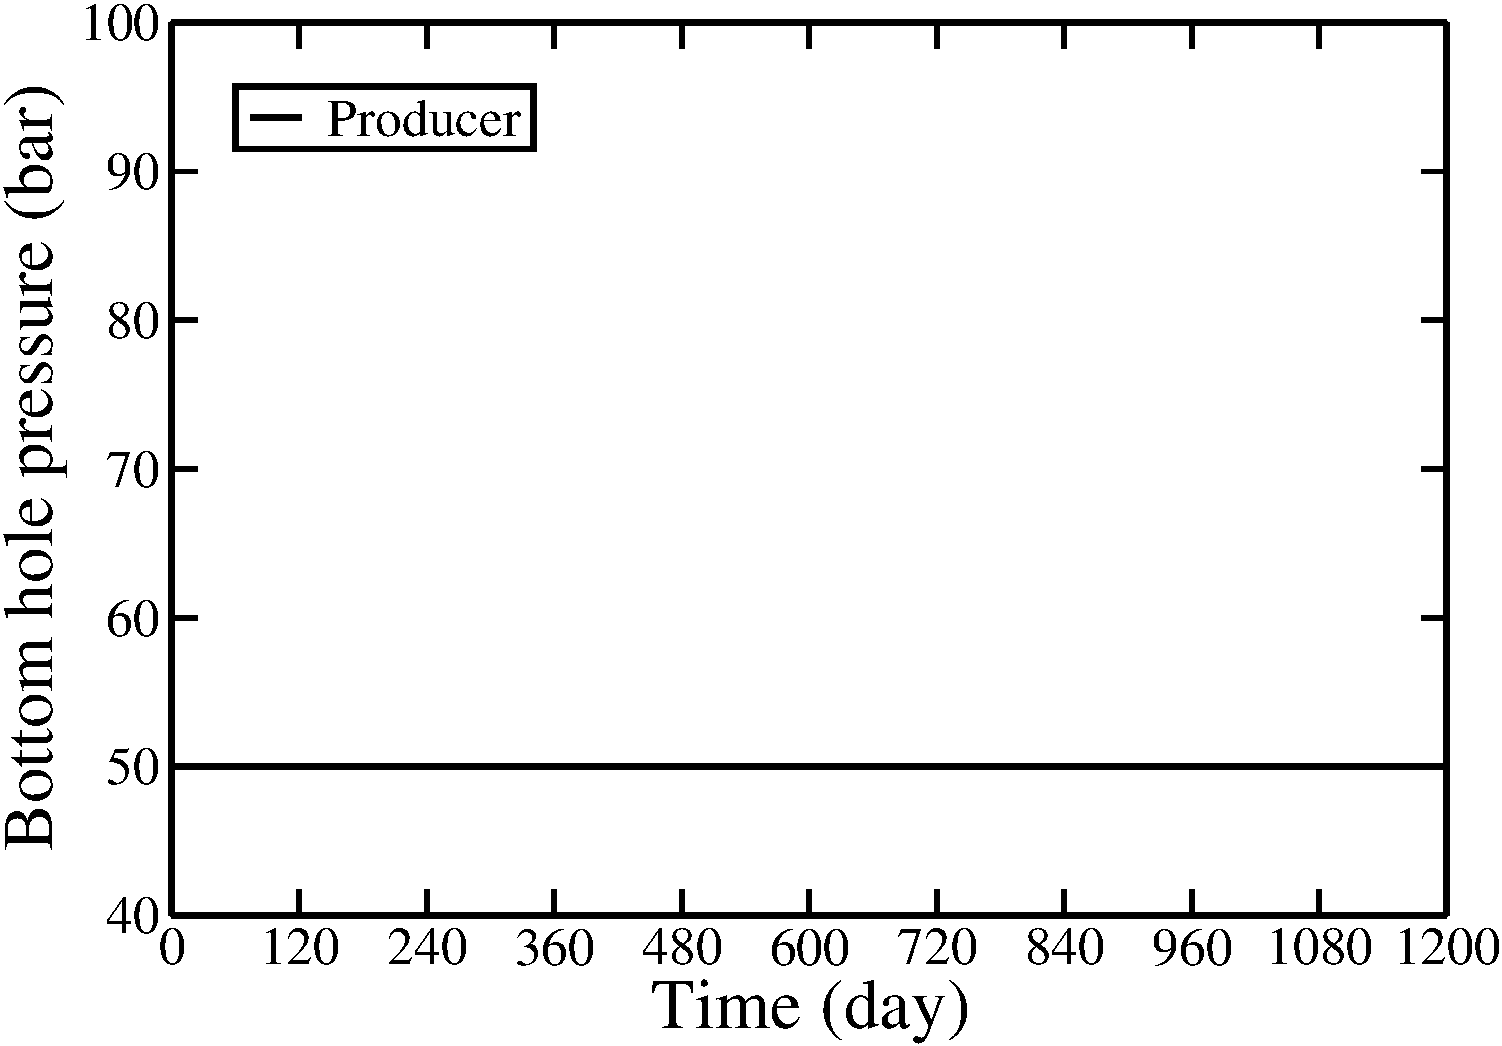
\includegraphics[height=2.7cm]{SimpleBHP_BHP.pdf}
    &
    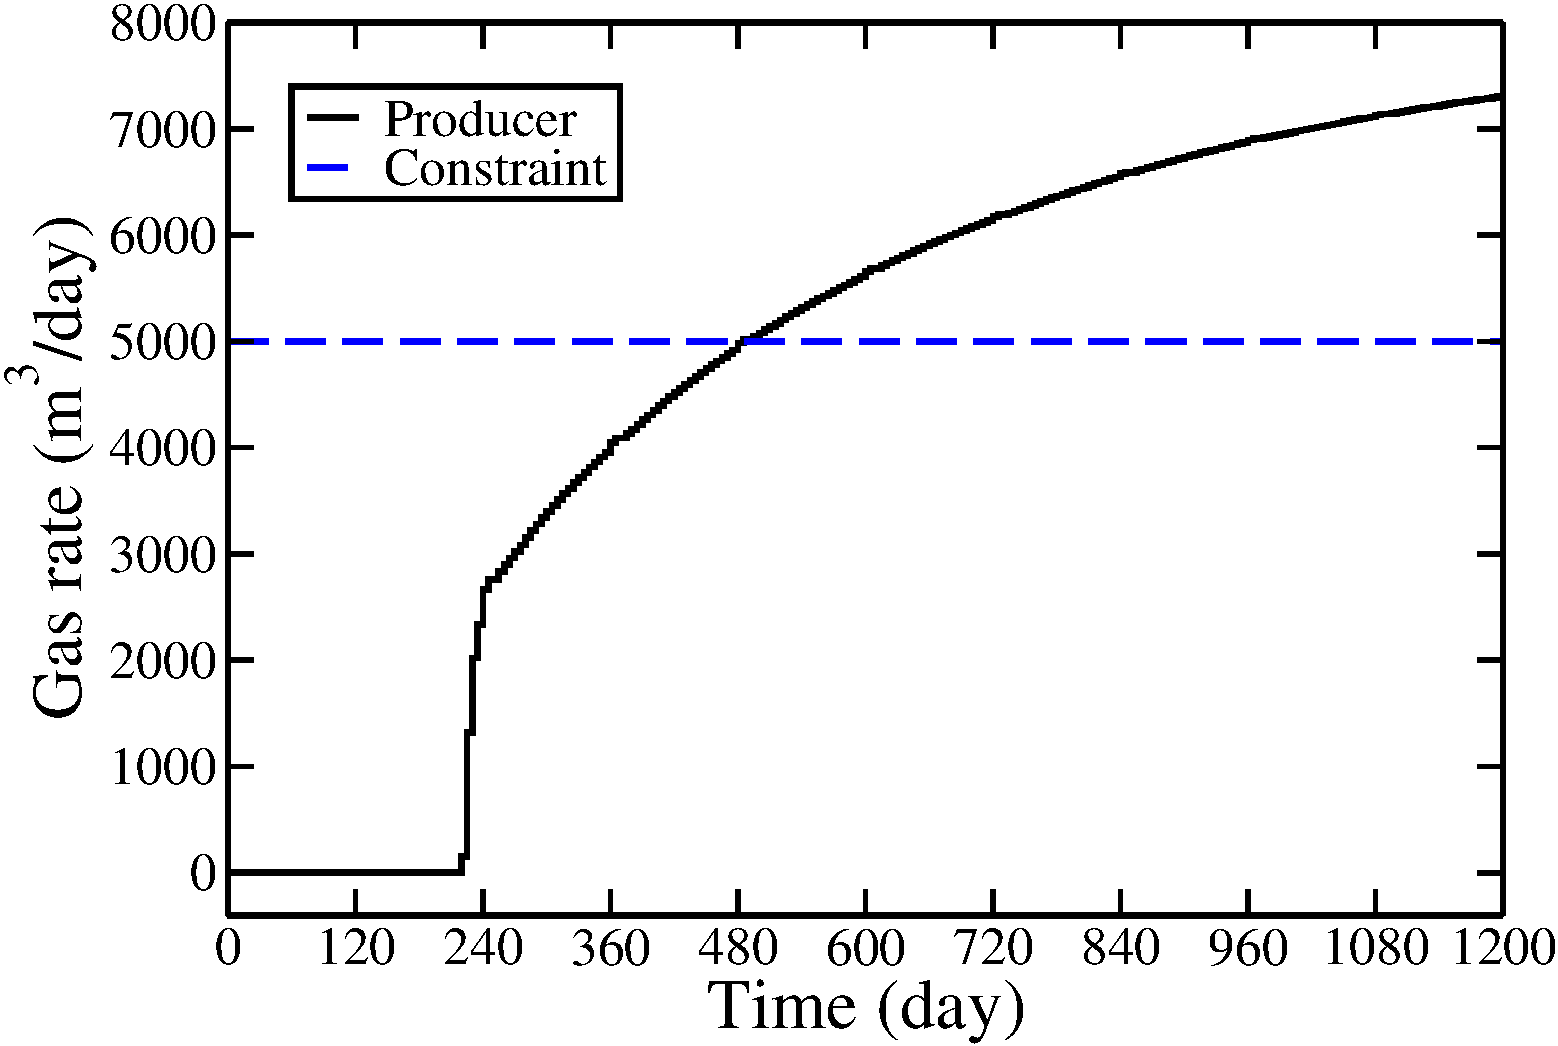
\includegraphics[height=2.7cm]{SimpleBHP_rate_gas.pdf} \\
    BHP & Rate control \\
    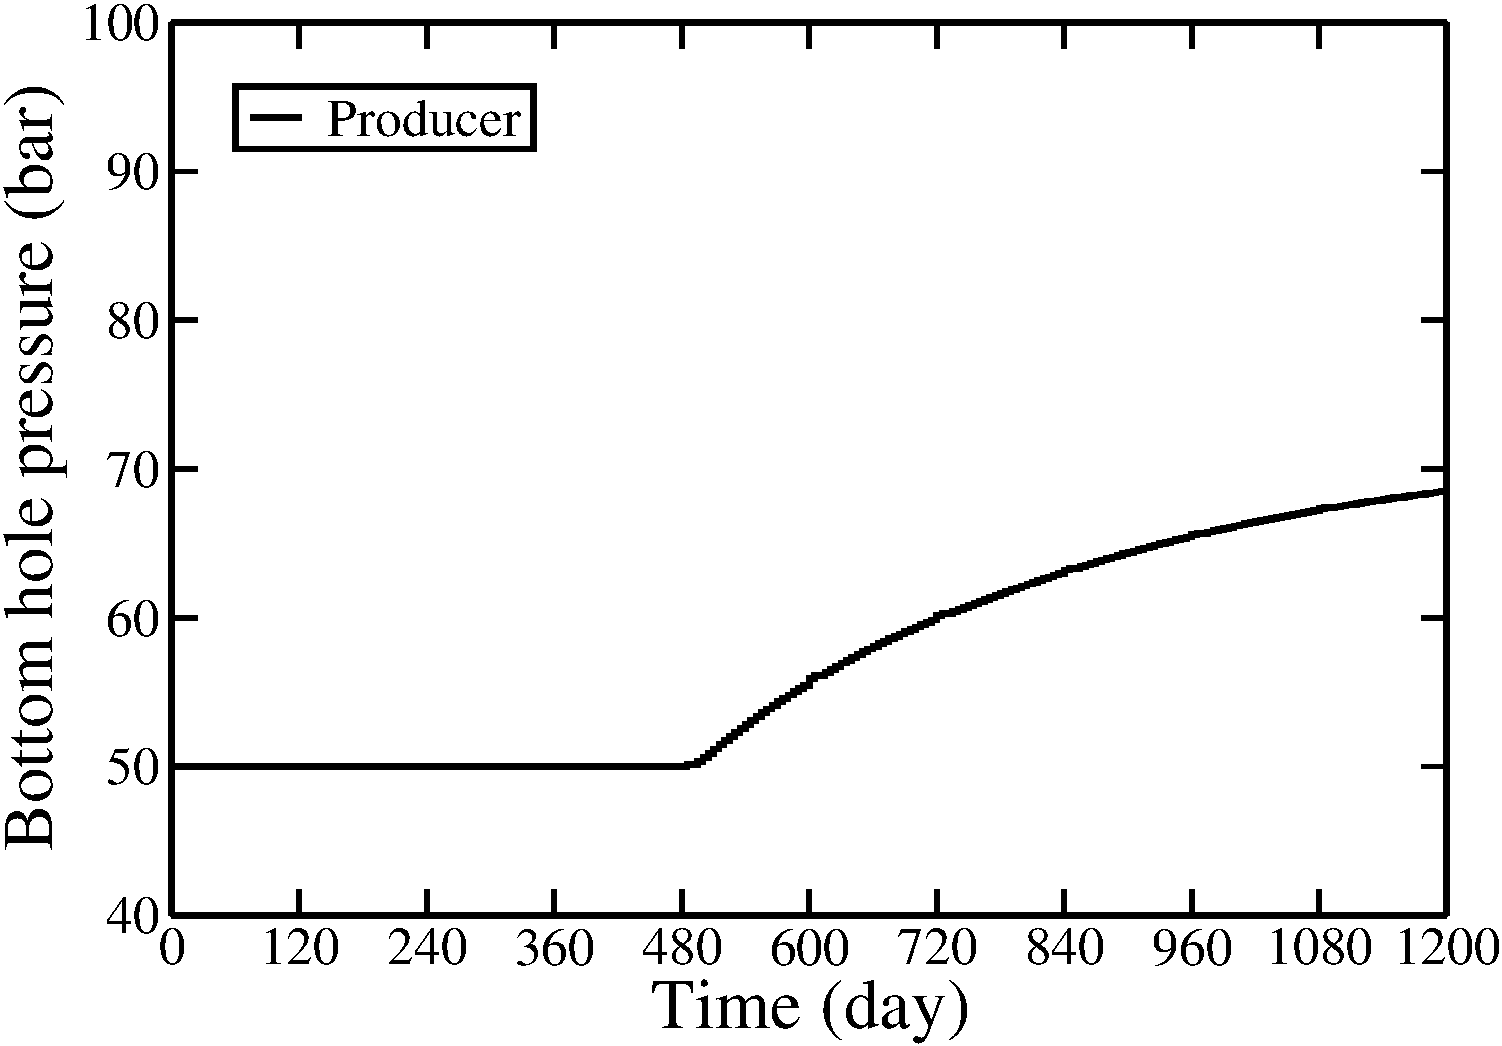
\includegraphics[height=2.7cm]{SimpleRate_BHP.pdf}
    &
    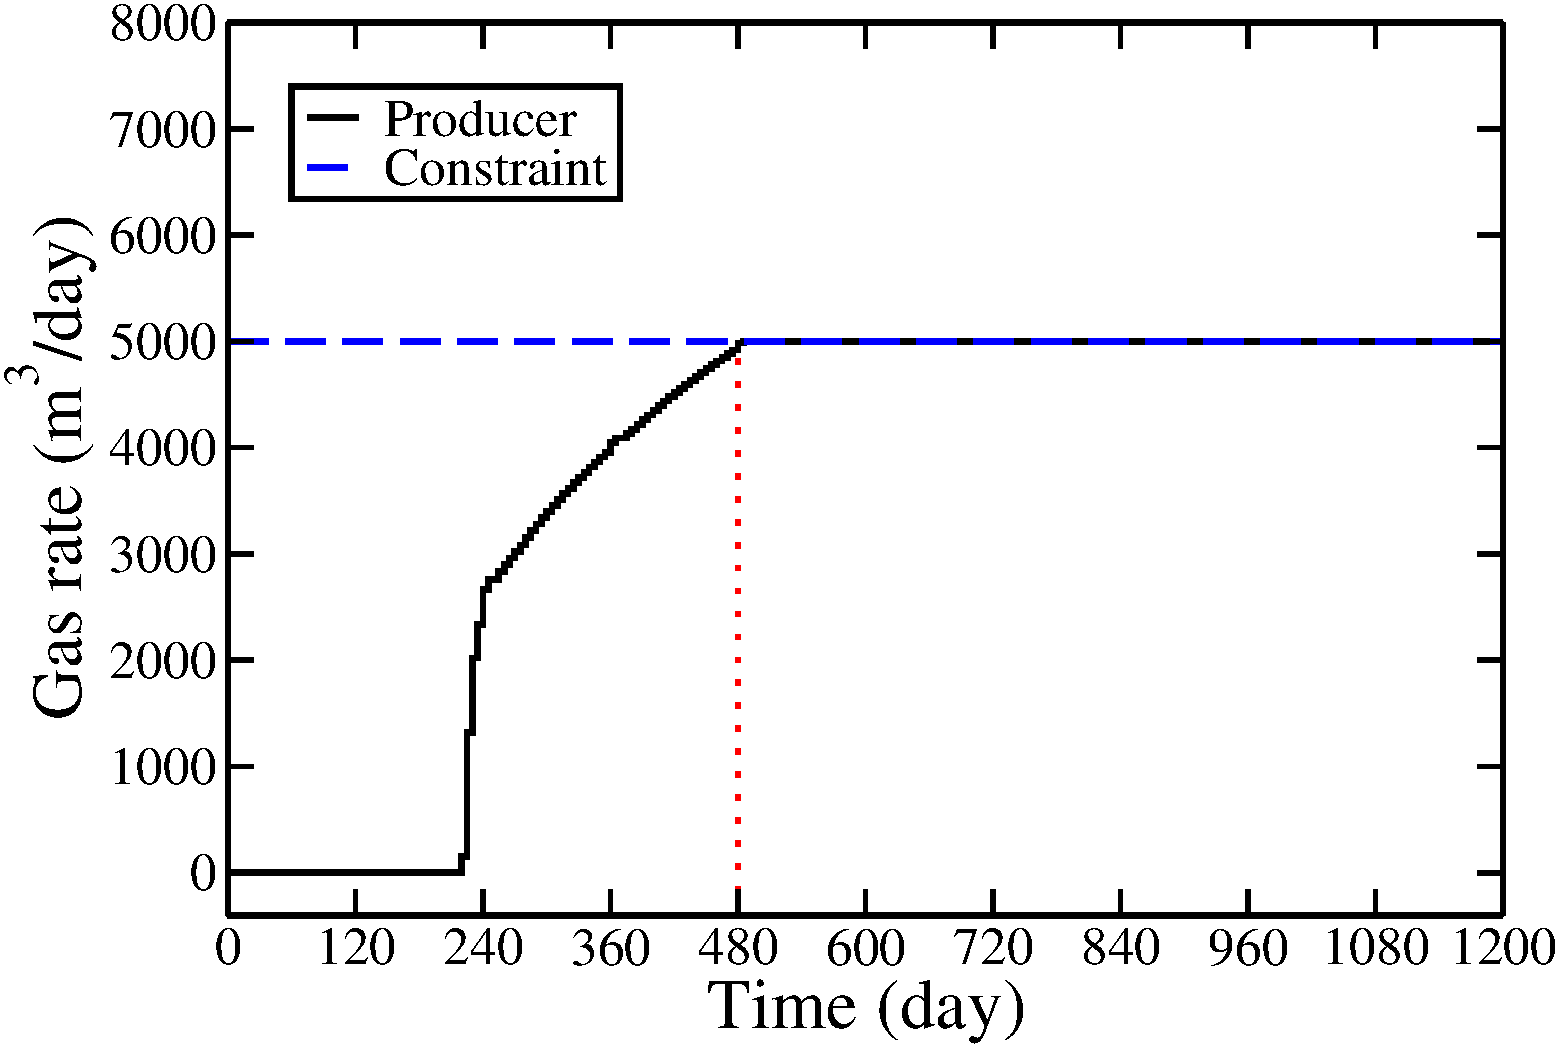
\includegraphics[height=2.7cm]{SimpleRate_rate_gas.pdf} \\
  \end{tabular}
\end{center}
     \caption{Schematic illustrating heuristic constraint handling. Top: Constant BHP and resulting gas rate. Bottom: BHP and gas rate satisfying constraint.}
\label{fig:BHPvsRateControl}
\end{figure}


Although it is clearly approximate, this heuristic constraint handling approach
has some potential advantages over the formal method described in
Section~\ref{sec:constr-opt}. For example, the heuristic treatment allows the
simulator to switch controls at any time step in the simulation, while the
formal approach only allows controls to switch at a relatively small number of
control steps (by way of comparison, in a typical problem we may have
  $O(10^2-10^3)$ time steps but only $O(10)$ control steps). The heuristic
approach thus enables, in some sense, a more `fine-grained' response, and it can
be viewed as having many more `control' variables (though these variables are
  not optimized formally). Increasing the number of control steps to provide the
same granularity to the optimizer as in the forward problem (i.e., setting the
  control step size to equal the time step size) should theoretically result in
better performance by the formal approach, though in practice the large
increase in the number of control variables would result in a much more difficult optimization
problem, which could negatively impact the performance of the optimizer. In the examples
below, we will compare the performance of these two approaches for handling
nonlinear constraints.

We note finally that if rates are used as the control variables, then the rate
constraints enter the optimization problem as simple bound constraints, which
are easy to satisfy. In this case, however, the BHPs become nonlinear
constraints. Our heuristic treatment would then entail the switch from rate
control to BHP control if the BHP constraint would otherwise be violated. We did
not test the performance of our procedure using rates as the control variables,
but this should be considered in future work.



\section{Numerical results}  \label{sec:results}

We will present results for four different cases. All involve bound and
nonlinear constraints, and we will compare the performance of the two approaches
described above for treating the nonlinear constraints. Because our
gradient-based optimization will find only a local optimum, we run each case
nine times, using a different initial guess for the well controls. Each initial
guess corresponds to a combination of BHPs from the set $\{p_I^u,p_I^l,p_I^a\}$
for the injectors and from the set $\{p_P^u,p_P^l,p_P^a\}$ for the producers,
where $p^u$, $p^l$ and $p^a$ designate the upper and lower limits on the
initial BHPs, and the average between these limits, respectively. We set
$p^l=p_{init}+1~{\rm bar}$ for the injectors and $p^u=p_{init}-1~{\rm bar}$
for the producers, where $p_{init}$ is the initial reservoir pressure. Note
that these `limits' are simply used to prescribe initial guesses for the
optimization -- they are not related to the actual BHP bound constraints.
For clarity, we will refer to each case by the number of the corresponding
run, as listed in Table~\ref{table:InitialGuesses}.



\begin{table}
\centering
\caption{Initial guesses for the optimizations for all
         cases considered}
\begin{tabular}{|c|c|}
\hline
Run & Initial guess    \\
\hline
1 & $[p_I^l, p_P^l]$ \\
2 & $[p_I^l, p_P^a]$ \\
3 & $[p_I^l, p_P^u]$ \\
4 & $[p_I^a, p_P^l]$ \\
5 & $[p_I^a, p_P^a]$ \\
6 & $[p_I^a, p_P^u]$ \\
7 & $[p_I^u, p_P^l]$ \\
8 & $[p_I^u, p_P^a]$ \\
9 & $[p_I^u, p_P^u]$ \\
\hline
\end{tabular}
  \label{table:InitialGuesses}
\end{table}





\subsection{Example 1 - $\Pi$ obstacle}

In the first example we maximize cumulative oil recovery under CO$_2$ injection. The two-dimensional geological model is depicted in Fig.~\ref{fig:PImodelPermeabilityMapAndWells}. A $\Pi$-shaped region is located at the center of a homogeneous reservoir. The model is discretized on a grid of dimensions $80\times80$. The permeability in most of the domain (red cells) is set to 4000~mD, while the permeability for the blue cells that comprise the $\Pi$-shaped region is set to $10^{-4}$~mD. Four injection wells are placed at the corners of the model, and the single production well is located inside the $\Pi$-shaped region. The model includes a total of four components (three hydrocarbon  components plus CO$_2$), as specified in Table~\ref{table:fluidForPImodel}. Further details on the reservoir model are provided in Table~\ref{table:PI}.

%
\begin{table}
\centering
\caption{Fluid description for Example 1}
\begin{tabular}{|l|r|r|r|r|}
\hline
Component            & CO$_2$ & C$_1$ & C$_4$ & C$_{10}$    \\
\hline
Initial composition (\%)  & 1    & 20  & 29    & 50 \\
Injection composition (\%)& 100   & - & - & - \\
\hline
\end{tabular}
\label{table:fluidForPImodel}
\end{table}
%

%
\begin{table}
\centering
\caption{Model parameters for Example 1}
\begin{tabular}{|l|rr|}
\hline
%\multicolumn{3}{|c|}{SPE10 top layer}  \\
%\hline
Grid size                & 80 $\times$ 80 $\times$ 1 &       \\
\hline\hline
Parameter                & Value    & Units \\
\hline
$\Delta x$               & 6 &m          \\
$\Delta y$               & 6 &m          \\
$\Delta z$               & 4&m         \\
Depth                    & 4000&m           \\
Initial pressure         & 100  & bar        \\
Temperature              &$100$ & $^\circ$C     \\
\hline
Rock compressibility     & $7.2 \times 10^{-5}$ & 1 / bar \\
Simulation time          &256 & d          \\
Pressure upper bound     & 120 & bar        \\
Pressure lower bound     &  90 & bar        \\
\hline
Residual gas saturation  & 0 & -            \\
Residual oil saturation  & 0 & -            \\
End point rel perm gas   & 1 & -            \\
End point rel perm oil   & 1 & -            \\
Corey exponent gas       & 2 & -            \\
Corey exponent oil       & 2 & -            \\
\hline\hline
Well locations [grid block no.] & $i$ & $j$     \\
\hline
Injector 1               &   1&  1   \\
Injector 2               &   1& 80   \\
Injector 3               &  80&  1   \\
Injector 4               &  80& 80   \\
Producer 1               &  40& 48   \\
\hline
\end{tabular}
\label{table:PI}
\end{table}
%


The control parameters in the optimization problem are the well BHPs. These are constrained to lie between an
upper bound of 120~bar and a lower bound of 90~bar. We additionally specify a
maximum (per-well) gas injection rate of 500~m$^3/$d at reservoir conditions.
The total simulation period is 256~days, and the well controls are determined
at initial time and for every subsequent 32-day interval. There are thus a
total of eight control steps and 40 control parameters.

Two reference solutions are generated. First, we run the
simulation with the production wells operating at the minimum BHP and the
injection wells at the maximum BHP. This solution is infeasible because it
violates the nonlinear output constraints (maximum gas injection rate of 500~m$^3/$d). Next, we apply the heuristic
constraint handling approach described above, with the maximum gas injection
rate set to 500~m$^3/$d. The cumulative oil production for these two cases is
given in the first row (`Reference') of Table~\ref{table:PiC500Steps8}. %Note that
%the values are very similar because the nonlinear constraint violation in the
%unconstrained case is small. 
The table headings refer to the treatment of the
nonlinear constraints -- bound constraints are satisfied in all cases.


We next perform optimizations that honor the bound constraints but not the
nonlinear constraints. The results for the nine runs, starting from different
initial guesses, are presented in Table~\ref{table:PiC500Steps8} in the column
labeled `Unconstr.' The best optimum achieved is a cumulative oil production of 190,200~m$^3$, obtained in Run~7.  This clearly exceeds the feasible reference result
of 152,200~m$^3$. Results using heuristic constraint handling are shown in
the third column. Here the best result is a cumulative oil production of 163,500~m$^3$ (Run~8), which exceeds the reference solution by 7.4\%. In the next set of runs we apply the formal constraint handling treatment. For
these runs, the best optimum is 160,600~m$^3$ of oil (Run~4). This value exceeds the reference solution by 5.5\%, but it is about 2\% less than that achieved using heuristic constraint handling. We will show below that results using the formal procedure can be improved through use of more control steps.


The oil production profiles for the best runs, along with the reference
(heuristic) case, are shown in Fig.~\ref{fig:PIRevenue}. Recall that
we are maximizing cumulative oil, so the fact that early time production in the
reference case exceeds that of the optimized cases is not of concern. The
detailed BHP and gas rate profiles for each case are shown in Figs.~\ref{fig:PIReferencePlots},
\ref{fig:PIHeuristicControls40Plots} and \ref{fig:PIFormalControls40Plots}. The oil rates for all three cases are depicted in Fig.~\ref{fig:PIOilRates}. Although the BHPs for the two
optimized cases are clearly different, the oil rate profiles do show some general
similarity. For example, they both show less variation in oil rate over the course of the simulation than the reference case.

It is important to note that the heuristic constraint handling approach is
more efficient computationally than the formal treatment. On average,
the formal approach required about three times the number of forward
simulations used in the corresponding heuristically constrained cases. This
large discrepancy results from the need to enforce feasibility within the
optimizer in the formal constraint handling approach.

We now assess the impact of using additional control variables. Theoretically, if the optimization problem remains sufficiently `tractable', as we increase the number of control variables the formal approach should (eventually) outperform the heuristic approach. However, if the optimization problem becomes significantly more difficult with increasing numbers of control variables (which may be related to the constraint lumping procedure applied), or if a large number of local optima associated with relatively poor objective function values appear, then it is not at all clear that the formal approach will outperform the heuristic treatment. 

To test the performance of our procedures, we now consider optimizations with 64 control steps, which corresponds to 320 control variables (the results above used eight control steps and 40 control variables). Results for this case are presented in Table~\ref{table:PiC500Steps64}. The best result using heuristic constraint handling provides cumulative oil production of 159,400~m$^3$ (Run~7). This is slightly lower than that achieved using 40 controls, which presumably reflects the fact that this is a more difficult optimization problem. Using the formal constraint handling approach, however, we achieve cumulative oil production of 170,200~m$^3$ (Run~1). This exceeds the feasible reference solution (152,500~m$^3$) by 11.6\%, which represents a substantial improvement. It also exceeds the best solution found using heuristic constraint handling (163,500~m$^3$ in Run~8, using 40 controls) by 4.1\%. In fact, three of the nine local optima achieved in this case using formal constraint handling exceed the best result obtained using heuristic constraint handling. These findings suggest that, for this case, the formal approach does indeed outperform the heuristic approach given a sufficient number of control variables.

Finally, it is worth noting that the spread in the results from run to run for (optimized) cumulative oil is larger with 320 control variables than it is with 40 control variables. In fact, with 320 control variables, optimizations using both constraint handling procedures lead to some local optima that are below the corresponding lowest optima achieved using 40 control variables (Runs~3 and 5 for the heuristic approach; Runs~2, 3 and 4 for the formal approach). Again, we believe this is indicative of the challenges associated with performing constrained optimization with increasing numbers of control variables.






\begin{figure}[ht]
\begin{center}
     \begin{tabular}{cccccccc}
      0.0001 &  500 & 1000 & 1500 & 2000 & 2500 & 3000 &4000
      \end{tabular}
      
\includegraphics[width=8cm, height=0.5cm]{VanEssenModelPermeabilityMapColorBar.png}
       
       \medskip

       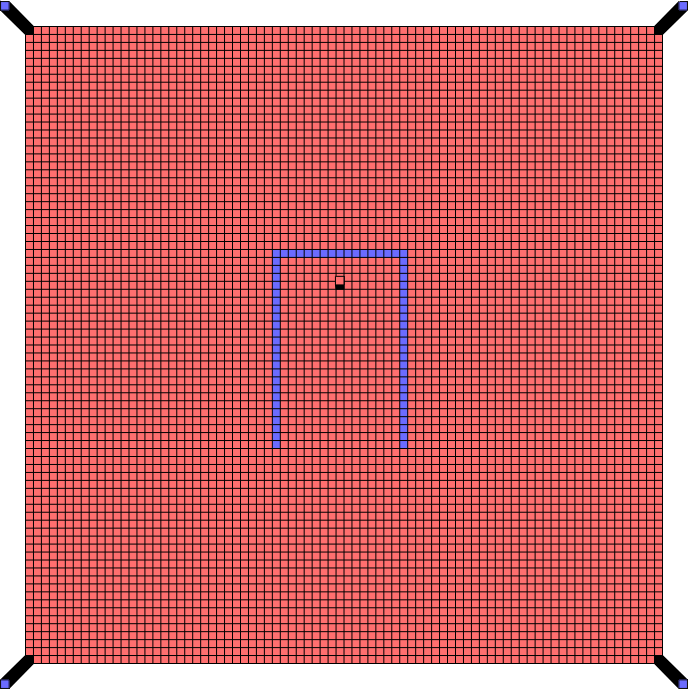
\includegraphics[totalheight=3.in]{PiPermeabilityMapAndWells.png} 
       \end{center}
     \caption{Injection wells (blue) and production well (red) for Example~1. Background shows $\tens{K}_x$ ($ \tens{K}_x = \tens{K}_y$).}
  \label{fig:PImodelPermeabilityMapAndWells}
\end{figure}



\begin{table}
\centering
\caption{Oil production in $10^3$~m$^3$ (Example 1, {\bf 40 control variables}) for the optimized objective function
         without satisfying the nonlinear constraints (`Unconstr.'), satisfying the nonlinear constraints
         using the heuristic treatment (`Heuristic'), and satisfying the nonlinear constraints
         using the formal approach (`Formal'). Best feasible results shown in bold.}
\begin{tabular}{|c|c|c|c|}
\hline
    & Unconstrained & Heuristic & Formal                       \\
\hline
Reference    & 163.9         &  152.2                      &                           \\
1                     & 187.5         &  156.6                      &        158.2        \\
2                     & 189.1         &  162.0                      &        146.2        \\
3                     & 177.3         &  149.0                      &        149.2        \\
4                     & 183.4         &  150.2                      & \bf{ 160.6 }      \\
5                     & 186.1         &  152.2                      &        152.9        \\
6                     & 185.0         &  158.9                      &        160.2        \\
7                     & 190.2         &  162.3                      &        142.5        \\ 
8                     & 190.1         &\bf{163.5}                 &        158.5        \\
9                     & 190.1         &     162.0                   &        158.0        \\
\hline
\end{tabular}
  \label{table:PiC500Steps8}
\end{table}

             
\begin{table}
\centering
\caption{Oil production in $10^3$~m$^3$ (Example 1, {\bf 320 control variables}) for the optimized objective function
         without satisfying the nonlinear constraints (`Unconstr.'), satisfying the nonlinear constraints
         using the heuristic treatment (`Heuristic'), and satisfying the nonlinear constraints
         using the formal approach (`Formal'). Best feasible results shown in bold.}
\begin{tabular}{|c|c|c|c|}
\hline
    & Unconstrained & Heuristic & Formal                          \\
\hline
Reference             & 150.1         &  152.5                      &                     \\
1                     & 188.1         &  149.9                      &  \bf{ 170.2 }        \\
2                     & 192.4         &  155.6                      &         131.4            \\
3                     & 186.5         &  136.4                      &         117.8          \\
4                     & 186.8         &  149.9                      &         133.7          \\
5                     & 186.5         &  142.2                      &         156.1          \\
6                     & 192.5         &  157.8                      &         168.2          \\
7                     & 192.5         &  \bf{159.4}               &         158.8          \\ 
8                     & 192.4         &  156.9                      &         161.1          \\
9                     & 192.2         &  157.0                      &         165.8          \\
\hline
\end{tabular}
  \label{table:PiC500Steps64}
\end{table}
 
 
 
 

 



%\begin{figure}[htb]
%\begin{center}
%     \begin{tabular}{ccccccccc}
%      0 &  0.125 & 0.250 & 0.375 & 0.500 & 0.625 & 0.750 & 0.875 & 1
%      \end{tabular}
%      
\includegraphics[width=8cm, height=0.5cm]{VanEssenModelPermeabilityMapColorBar.png}
%       
%       \medskip
%
%       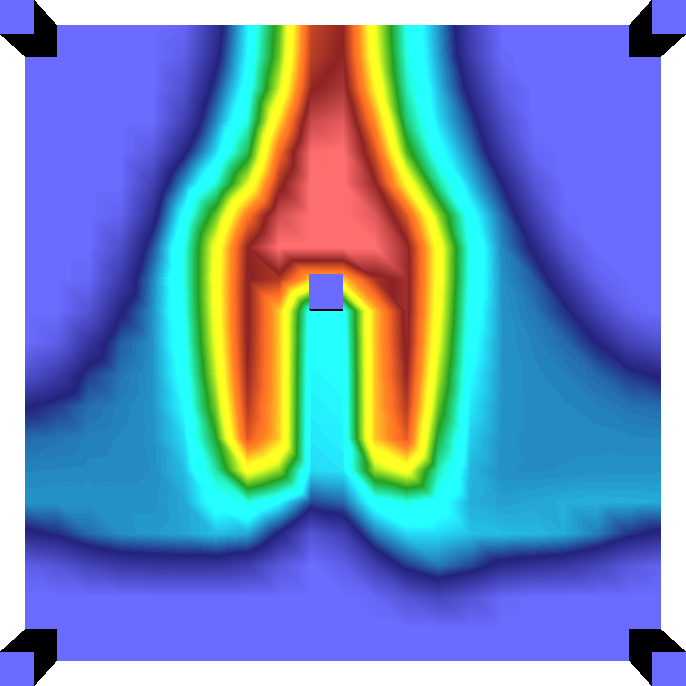
\includegraphics[totalheight=3.in]{PiBenchmarkSteps256RefenceC500T256.png} 
%
%       \medskip
%
%       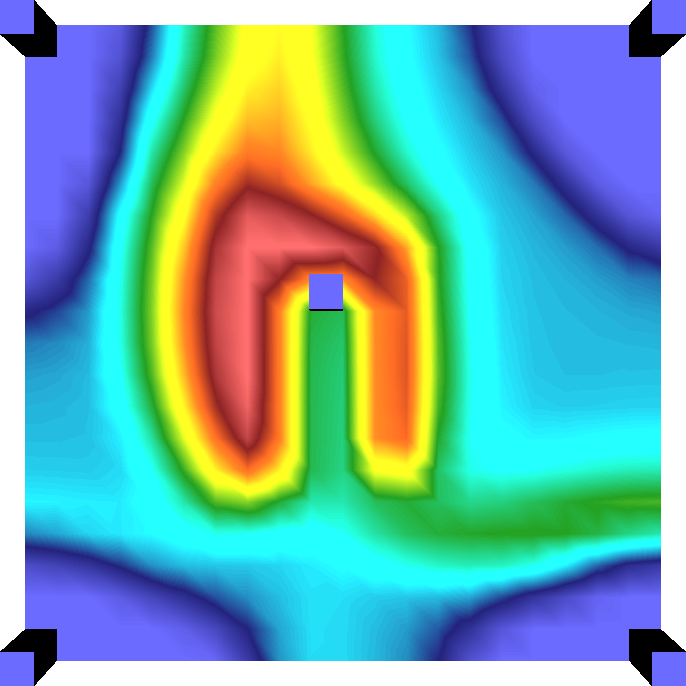
\includegraphics[totalheight=3.in]{PiBenchmarkSteps256HeuristicC500T256.png} 
%
%       \medskip
%
%       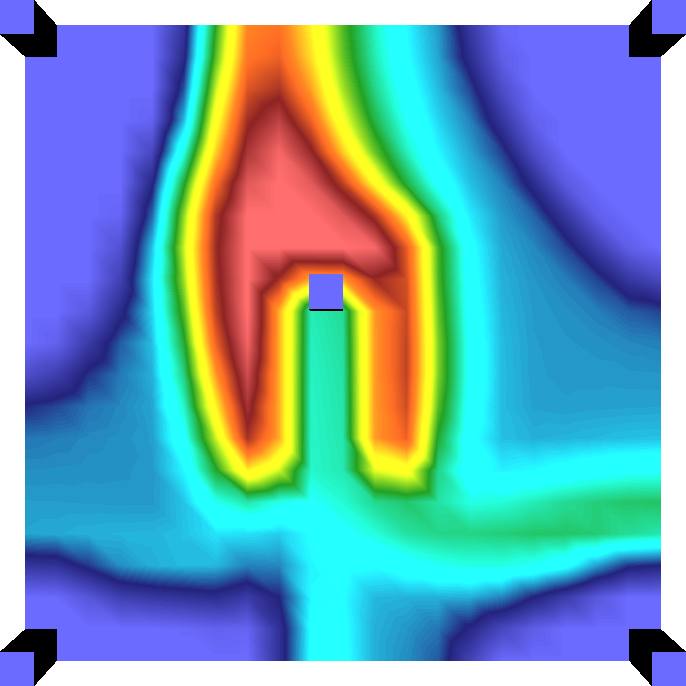
\includegraphics[totalheight=3.in]{PiBenchmarkSteps256FormalC500T256.png} 
%
%       \end{center}
%     \caption{Injection wells (blue) and production wells (red) for Example 1. Background shows $\tens{K}_x$ ($ \tens{K}_x = \tens{K}_y$).}
%  \label{fig:PImodelOilSaturation}
%\end{figure}

\begin{figure} [ht]
\begin{center}
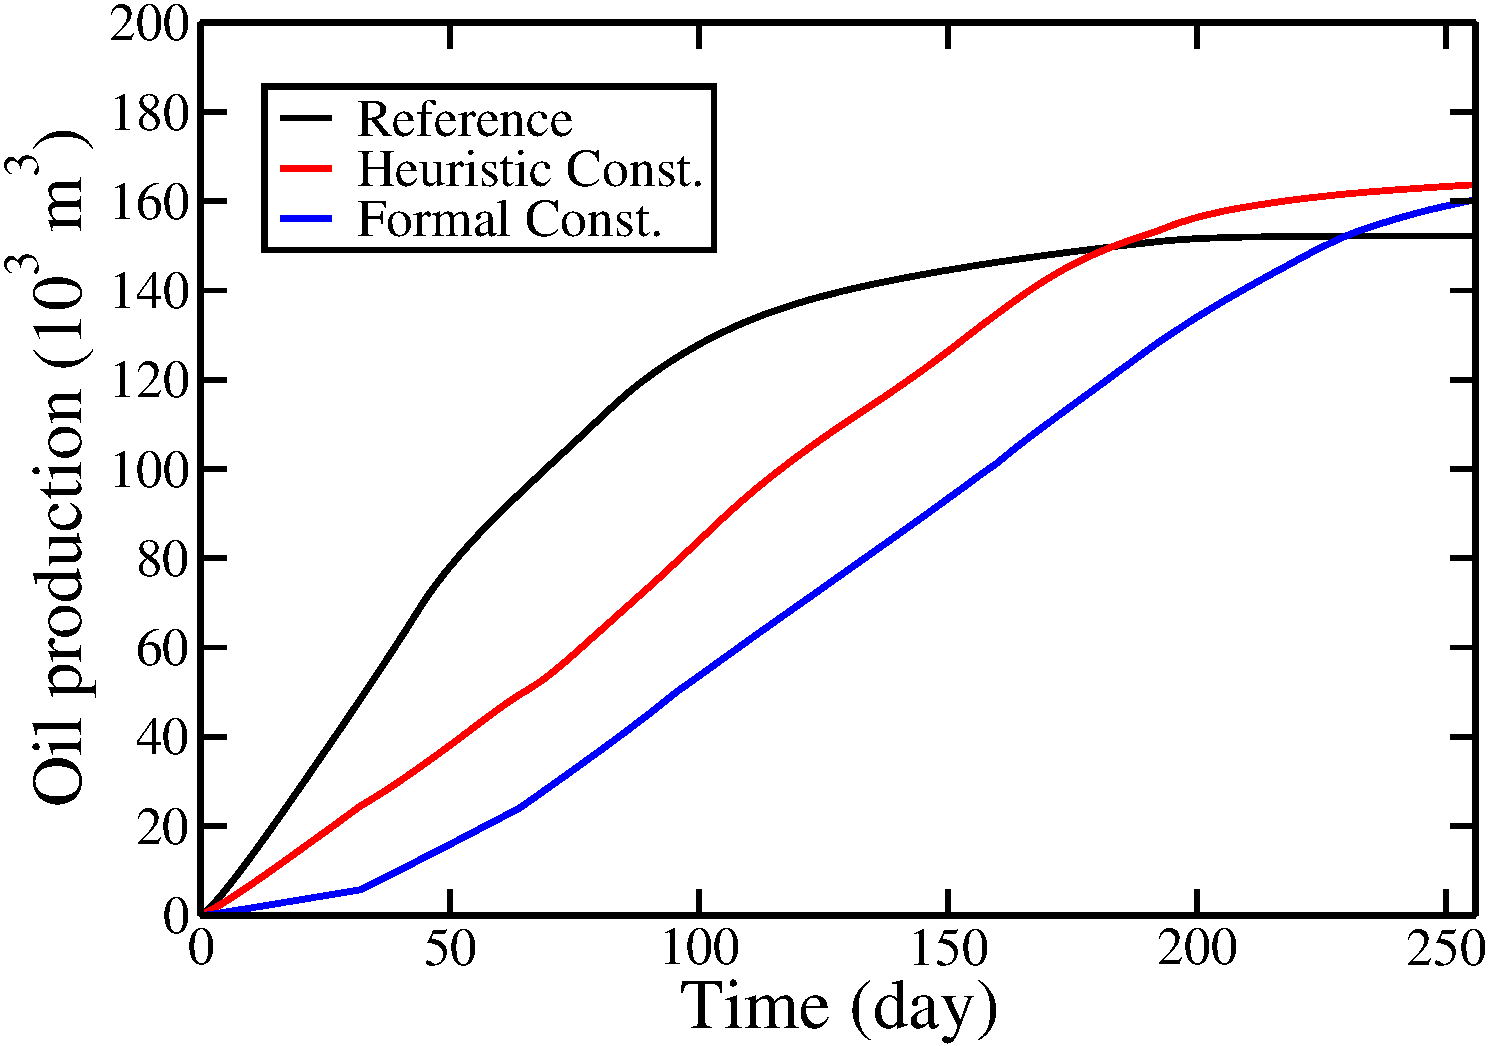
\includegraphics[totalheight=2.17in,angle=0]{RevenuePI2.pdf}
\end{center}
\caption{Oil production versus time (Example 1, 40 control variables). Results are for
  feasible reference case (black curve), best heuristically constrained solution (Run 8, red curve)
  and best formally constrained solution (Run 4, blue curve).}
\label{fig:PIRevenue}
\end{figure}
\begin{figure}
\begin{center}
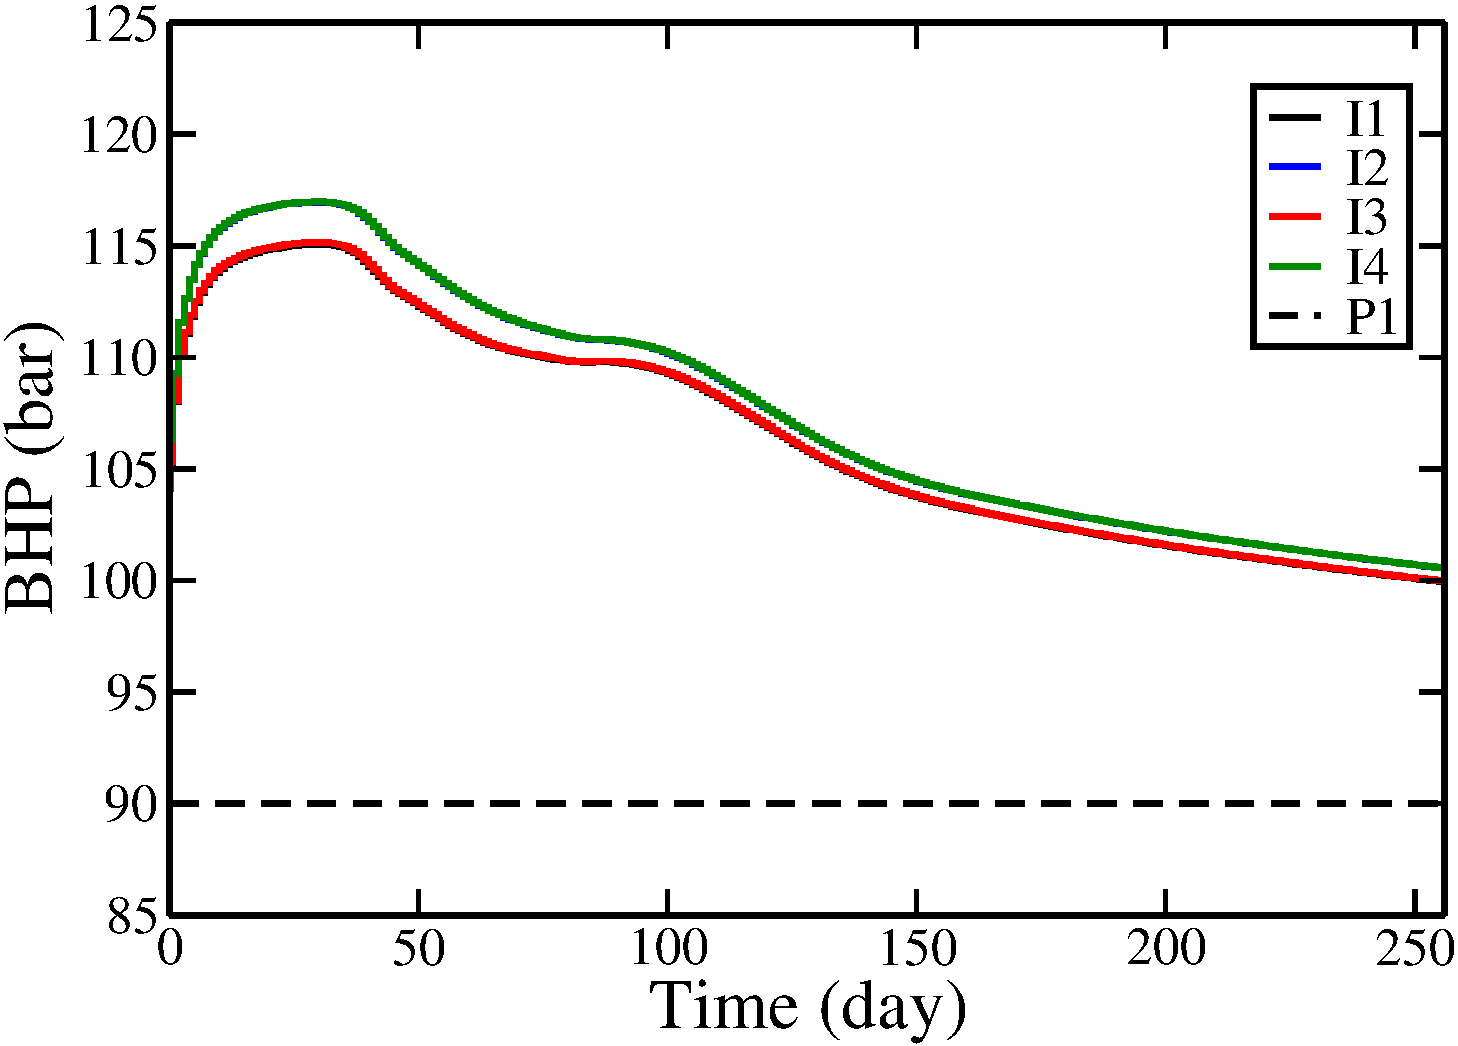
\includegraphics[totalheight=2.2in,angle=0]{ReferenceC500HeuristicItPb_BHP.pdf}
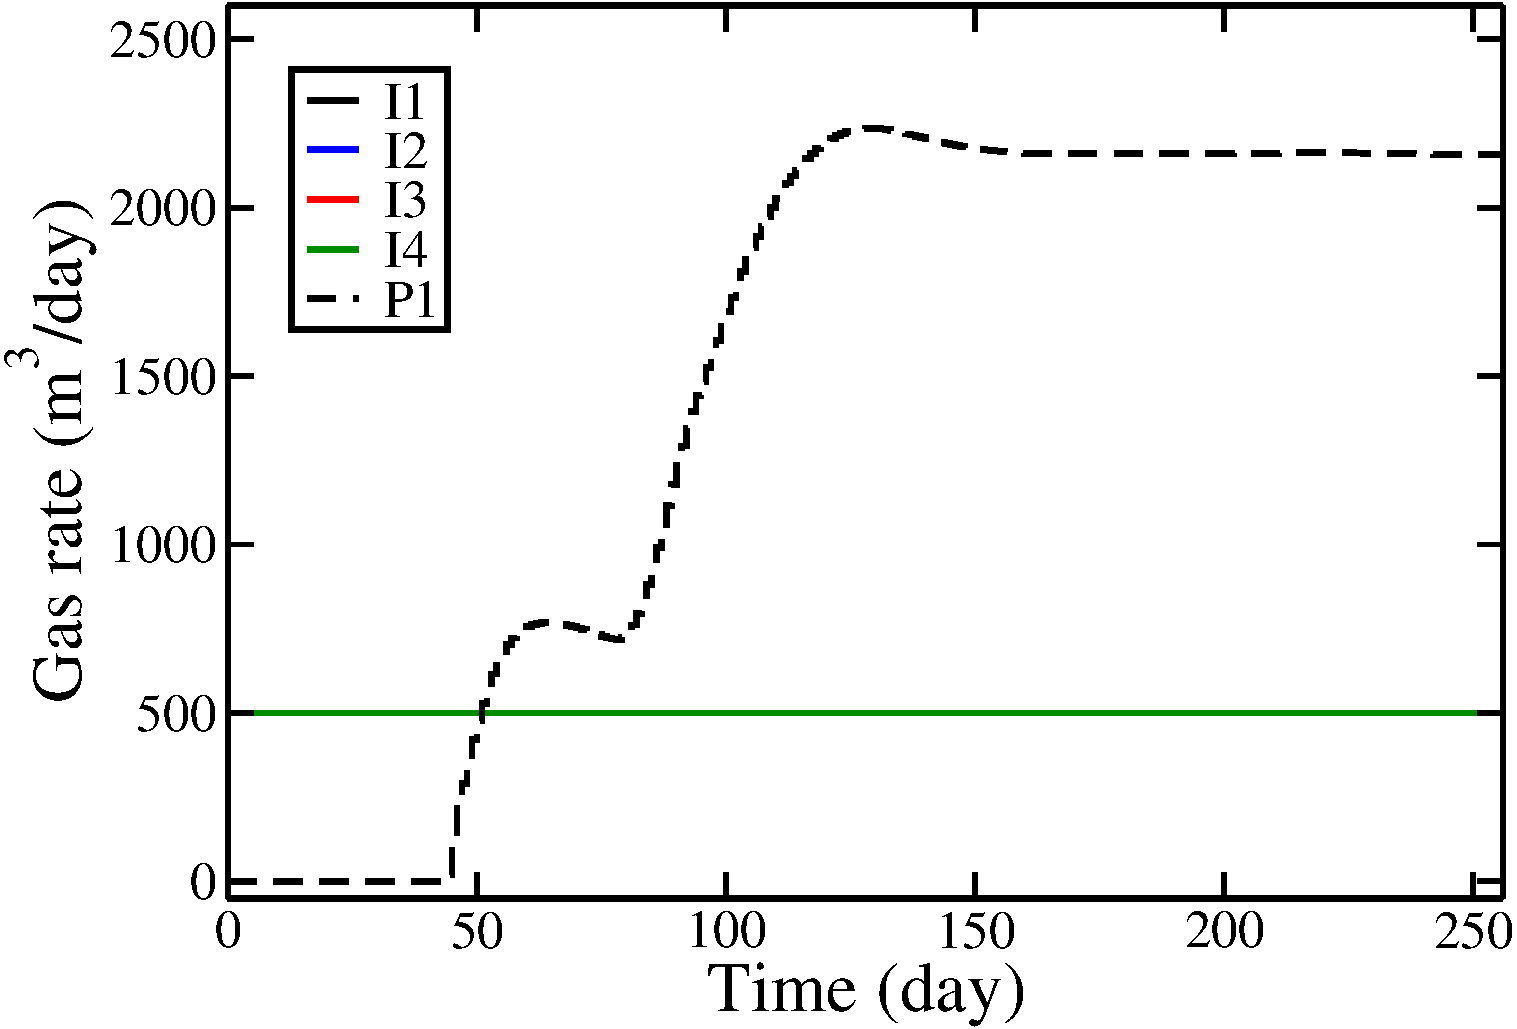
\includegraphics[totalheight=2.17in,angle=0]{ReferenceC500HeuristicItPb_rate_gas.pdf}
\end{center}
\caption{BHPs (top) and gas rates (bottom) for the feasible reference solution (Example 1).}
\label{fig:PIReferencePlots}
\end{figure}




%%%%%%%%%%%%%%%%%%%%%%%%%%% Pi 40 controls    %%%%%%%%%%%%%%%%%%%%%%%%%%%%%%

\begin{figure}
\begin{center}
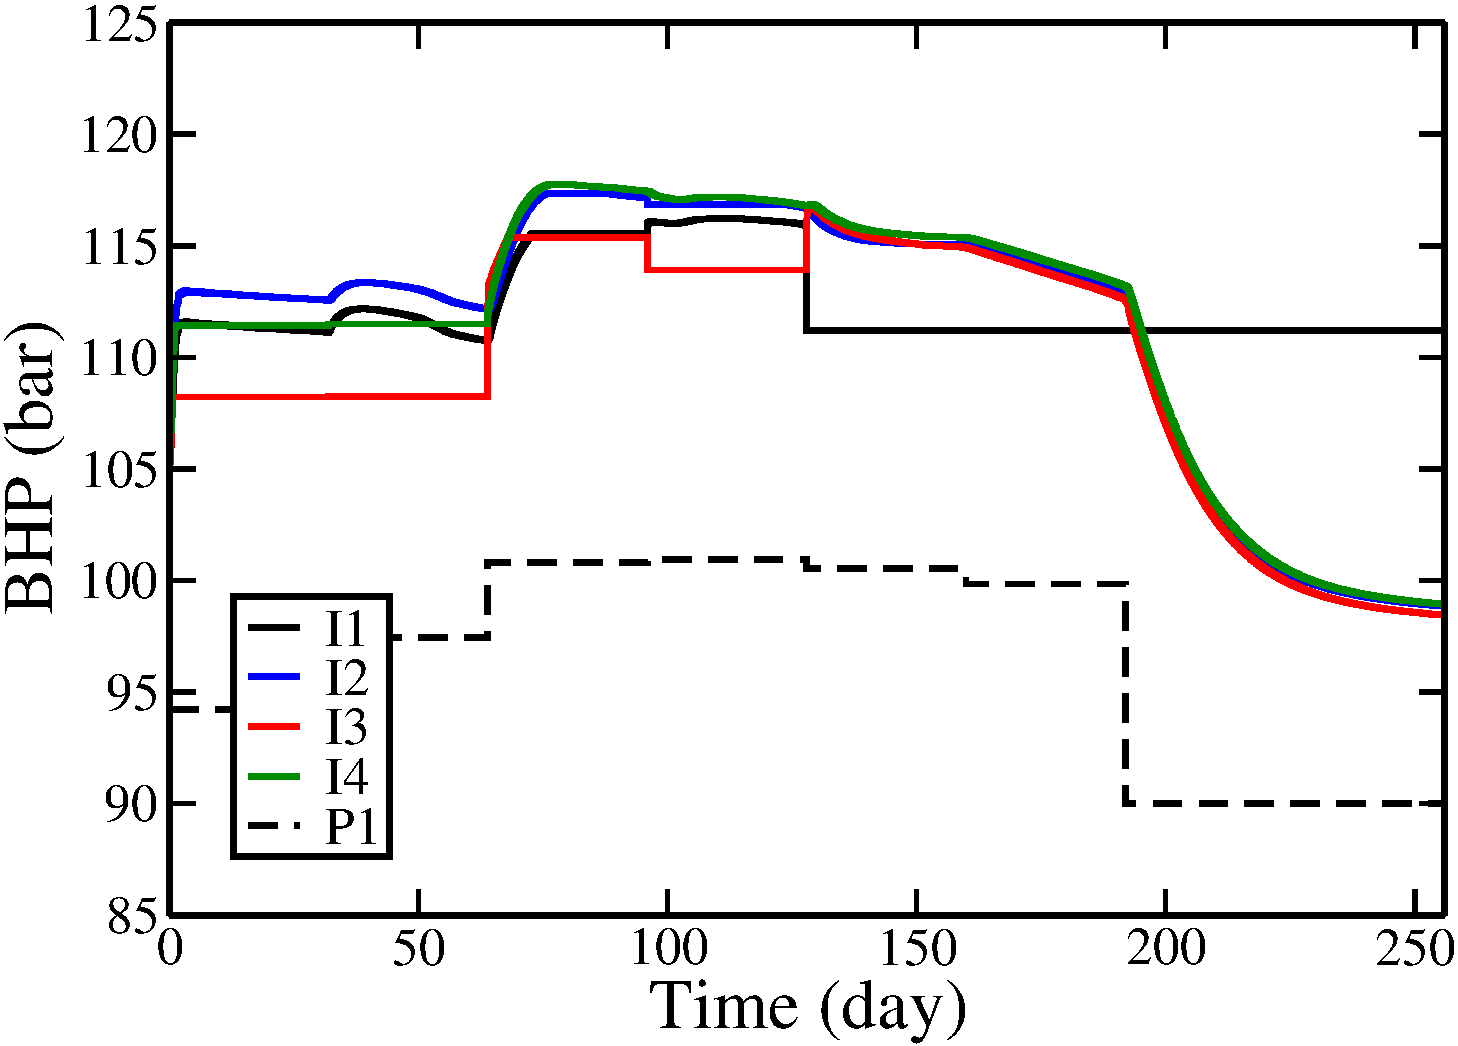
\includegraphics[totalheight=2.2in,angle=0]{HeuristicC500Steps8OptimalItPm_BHP.pdf}
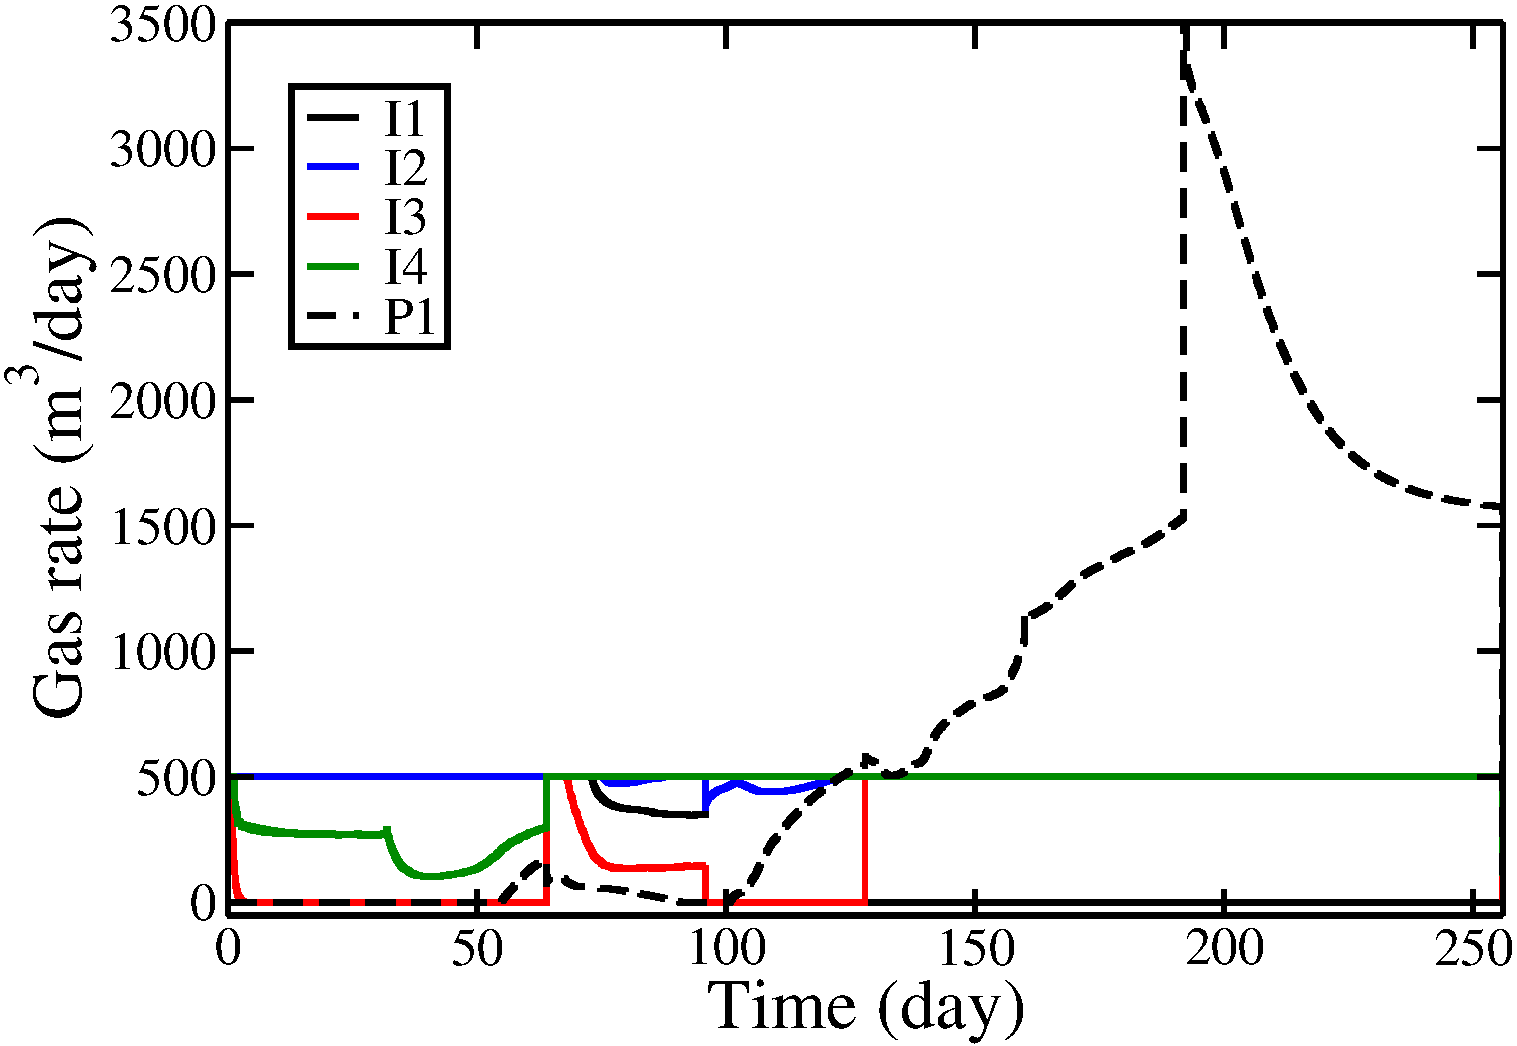
\includegraphics[totalheight=2.17in,angle=0]{HeuristicC500Steps8OptimalItPm_rate_gas.pdf}
\end{center}
\caption{BHPs (top) and gas rates (bottom) for the best heuristically constrained solution using 40 controls (Example 1, Run 8).}
\label{fig:PIHeuristicControls40Plots}
\end{figure}

\begin{figure}
\begin{center}
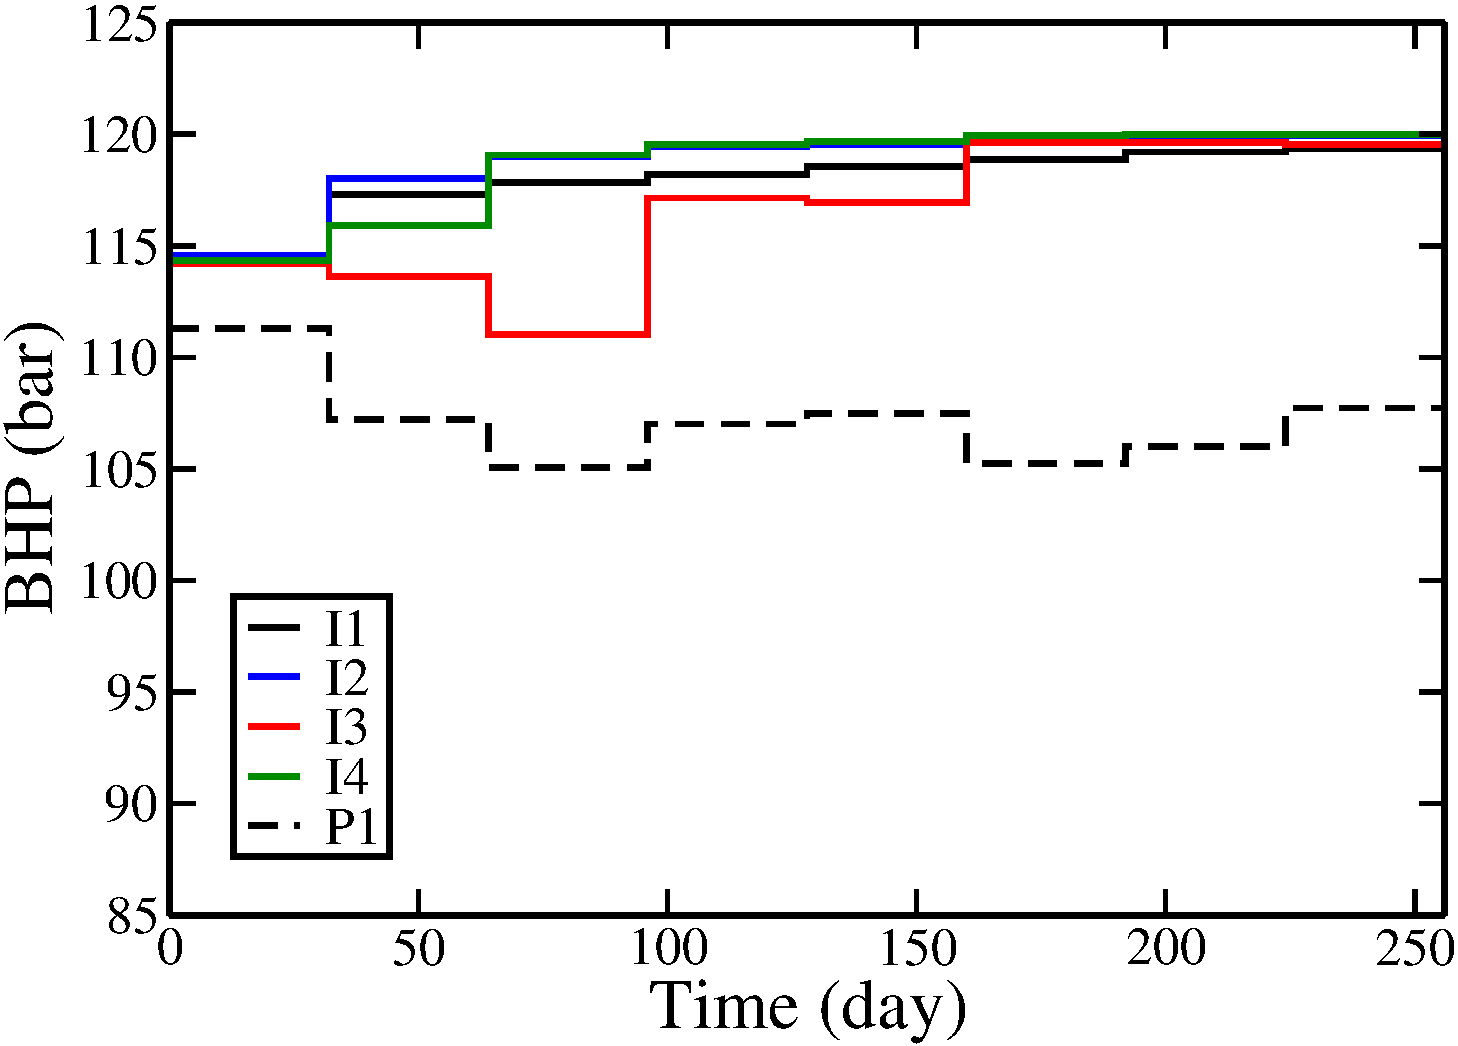
\includegraphics[totalheight=2.2in,angle=0]{FormalC550Steps8OptimalImPb_BHP.pdf}
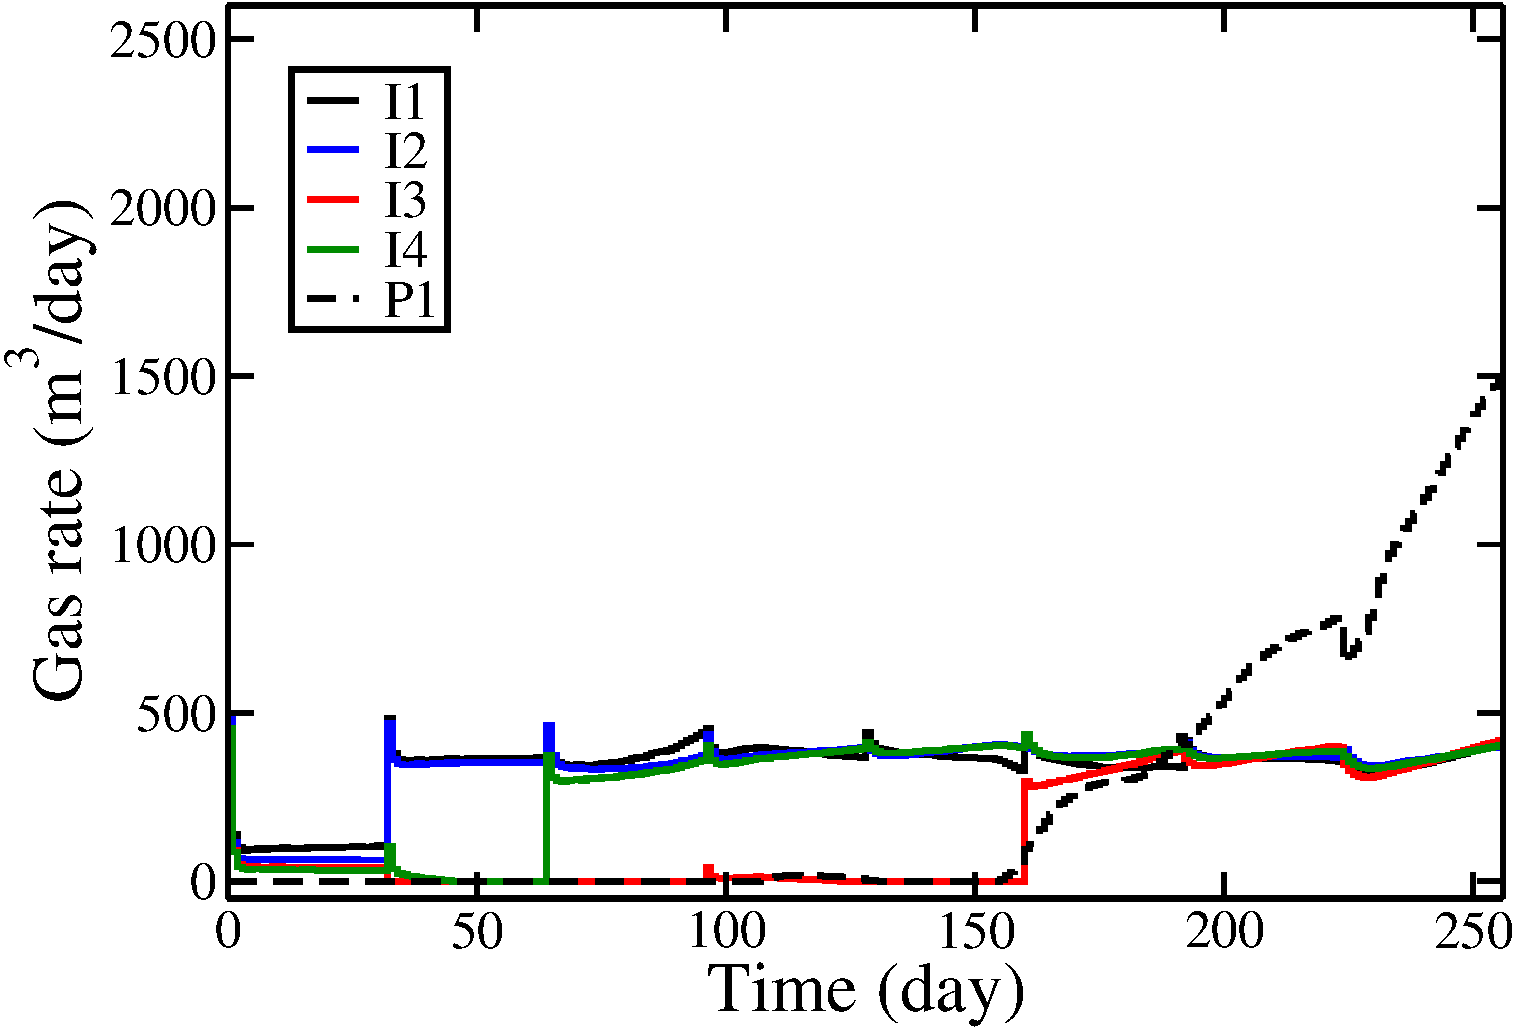
\includegraphics[totalheight=2.17in,angle=0]{FormalC550Steps8OptimalImPb_rate_gas.pdf}
\end{center}
\caption{BHPs (top) and gas rates (bottom) for the best formally constrained solution using 40 controls (Example 1, Run 4).}
\label{fig:PIFormalControls40Plots}
\end{figure}

%%%%%%%%%%%%%%%%%%%%%%%%%%%%%%%%%%%%%%%%%%%%%%%%%%%%%%%%%%%%%%%%%%%%%%%%%%%%




%%%%%%%%%%%%%%%%%%%%%%%%%%% Pi 320 controls   %%%%%%%%%%%%%%%%%%%%%%%%%%%%%%

%\begin{figure}
%\begin{center}
%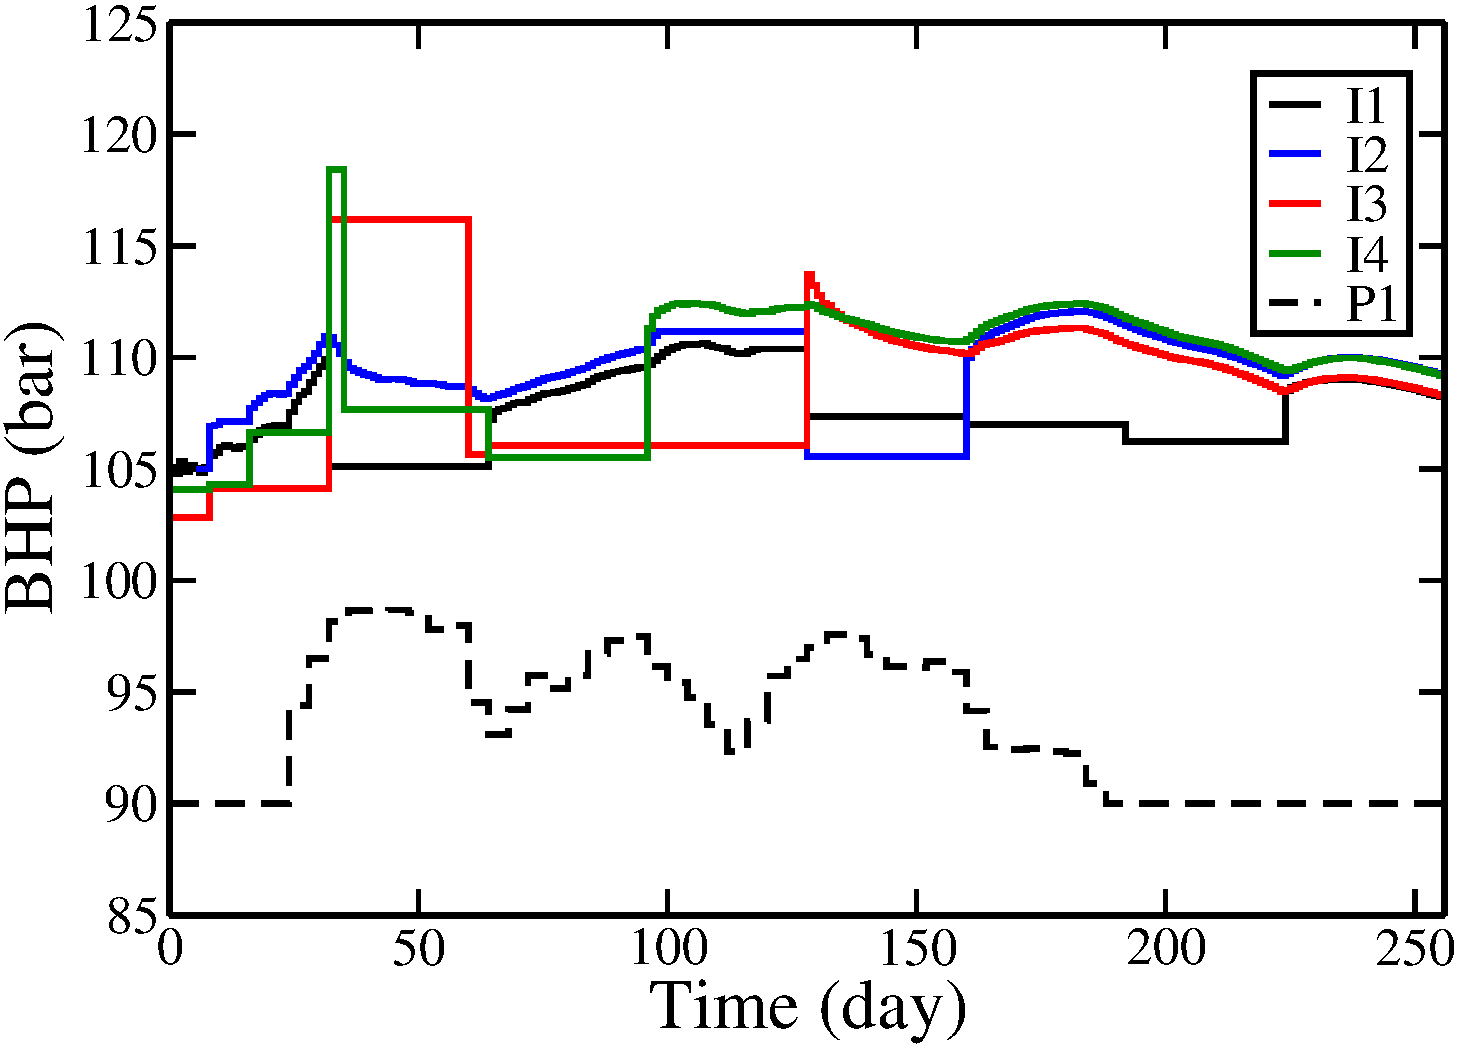
\includegraphics[totalheight=2.2in,angle=0]{HeuristicC500Steps64OptimalImPb_BHP.pdf}
%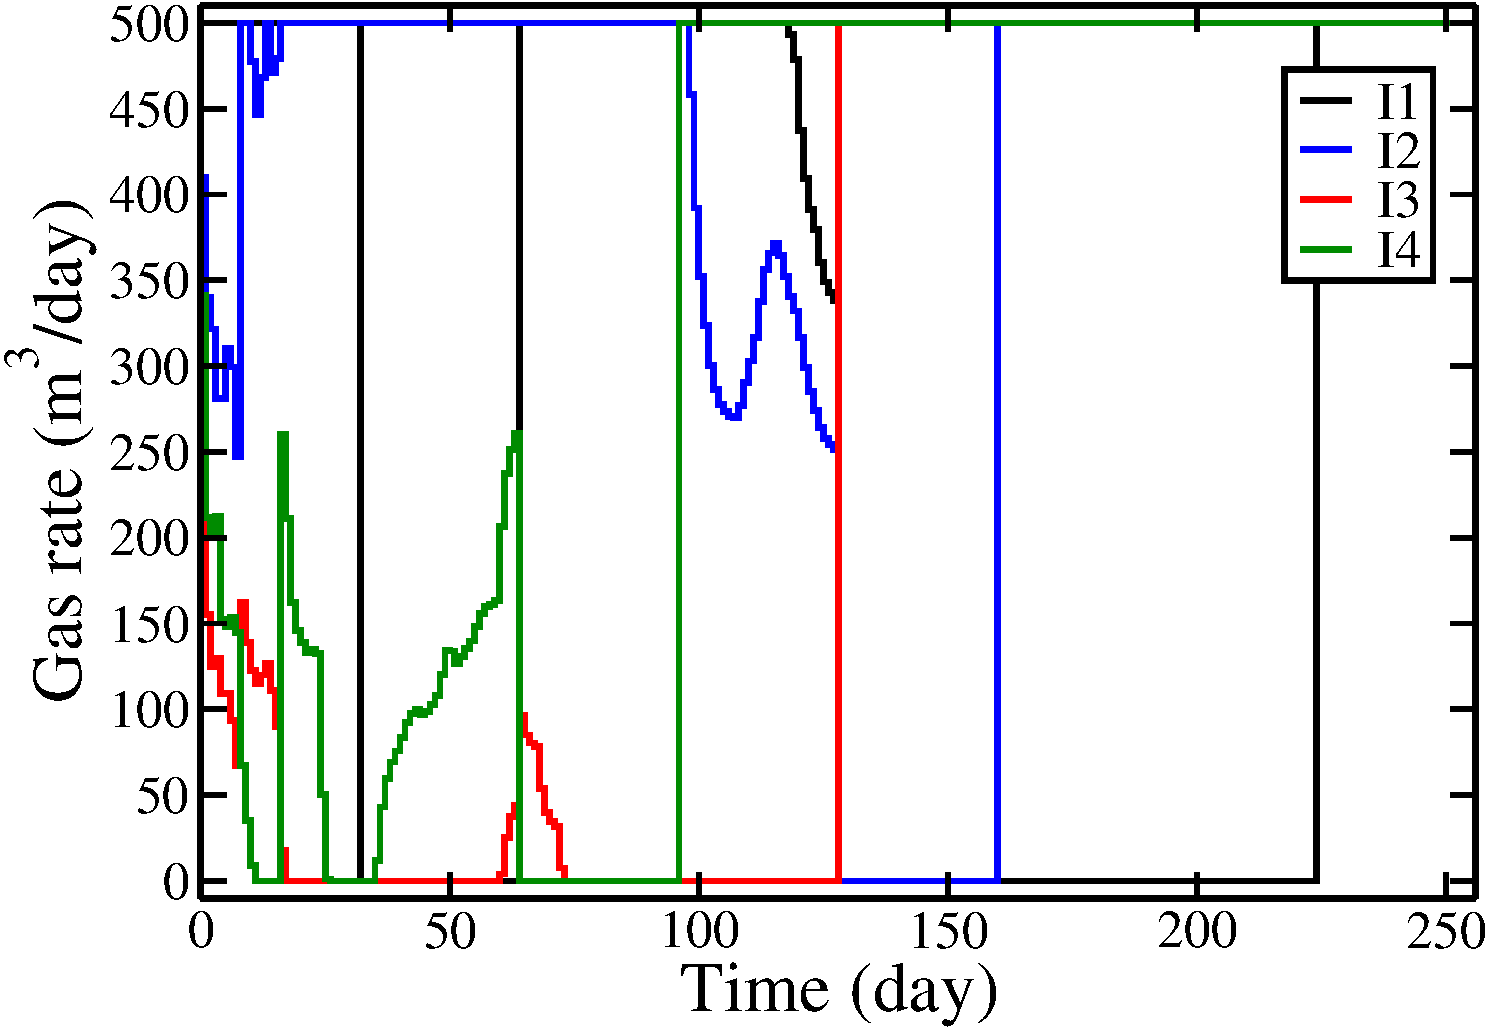
\includegraphics[totalheight=2.17in,angle=0]{HeuristicC500Steps64OptimalImPb_rate_gas.pdf}
%\end{center}
%\caption{BHPs (top) and gas rates (bottom) for the best heuristically constrained solution using 320 controls (Example 1, Run 4).}
%\label{fig:PIHeuristicControls320Plots}
%\end{figure}


%\begin{figure}
%\begin{center}
%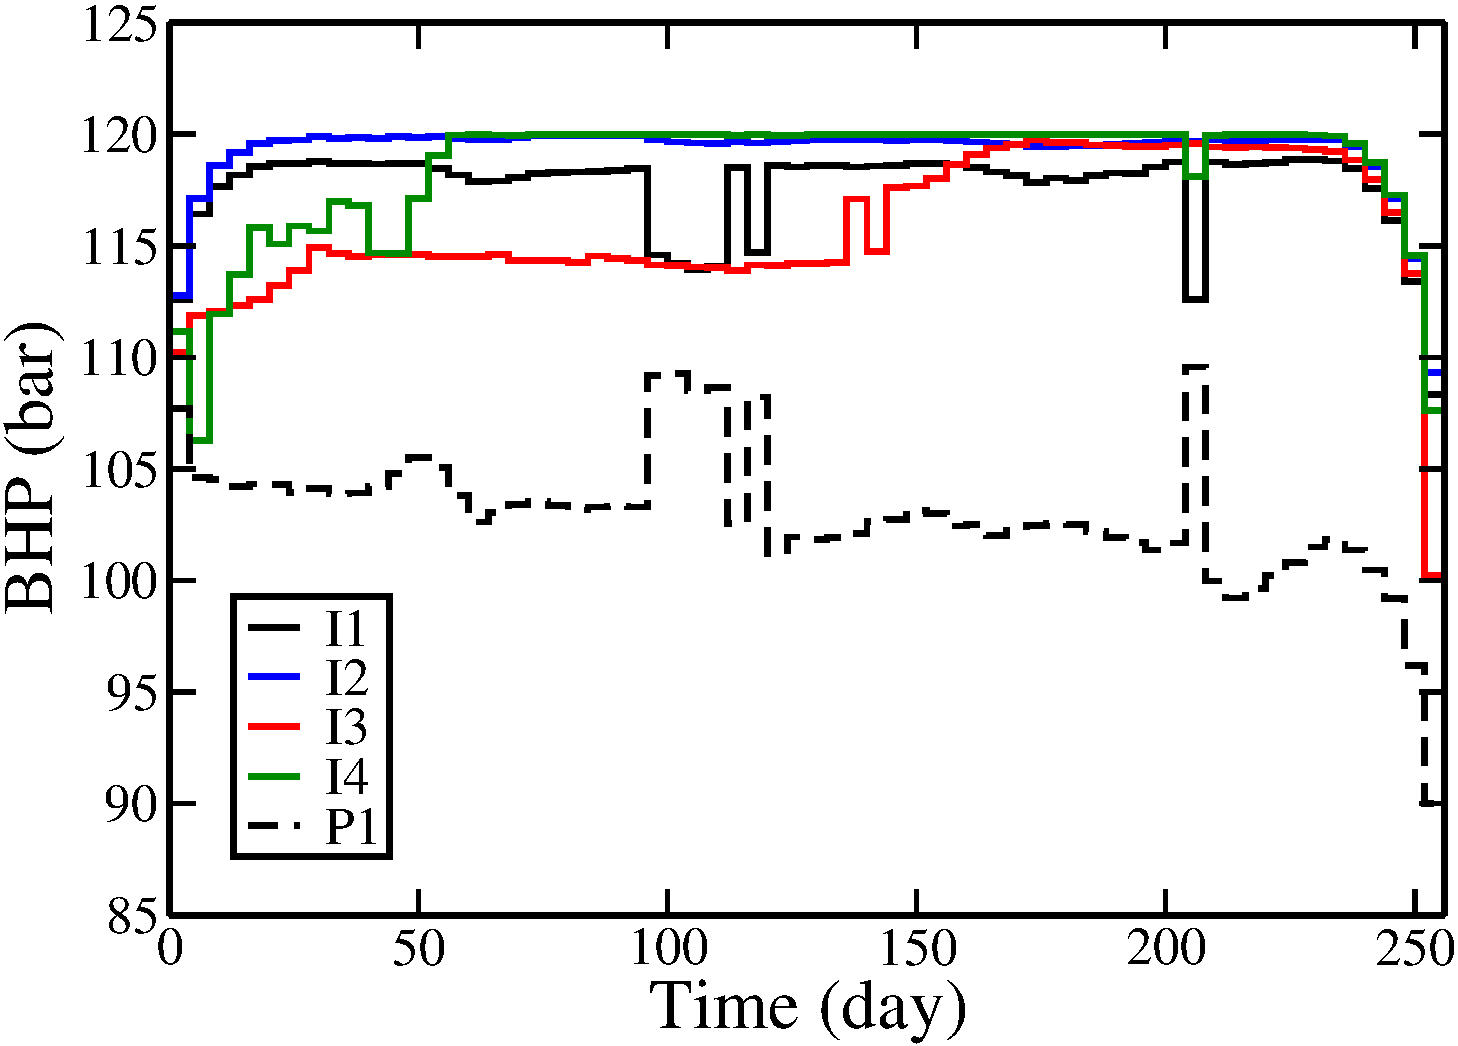
\includegraphics[totalheight=2.2in,angle=0]{FormalC600Steps64OptimalItPb_BHP.pdf}
%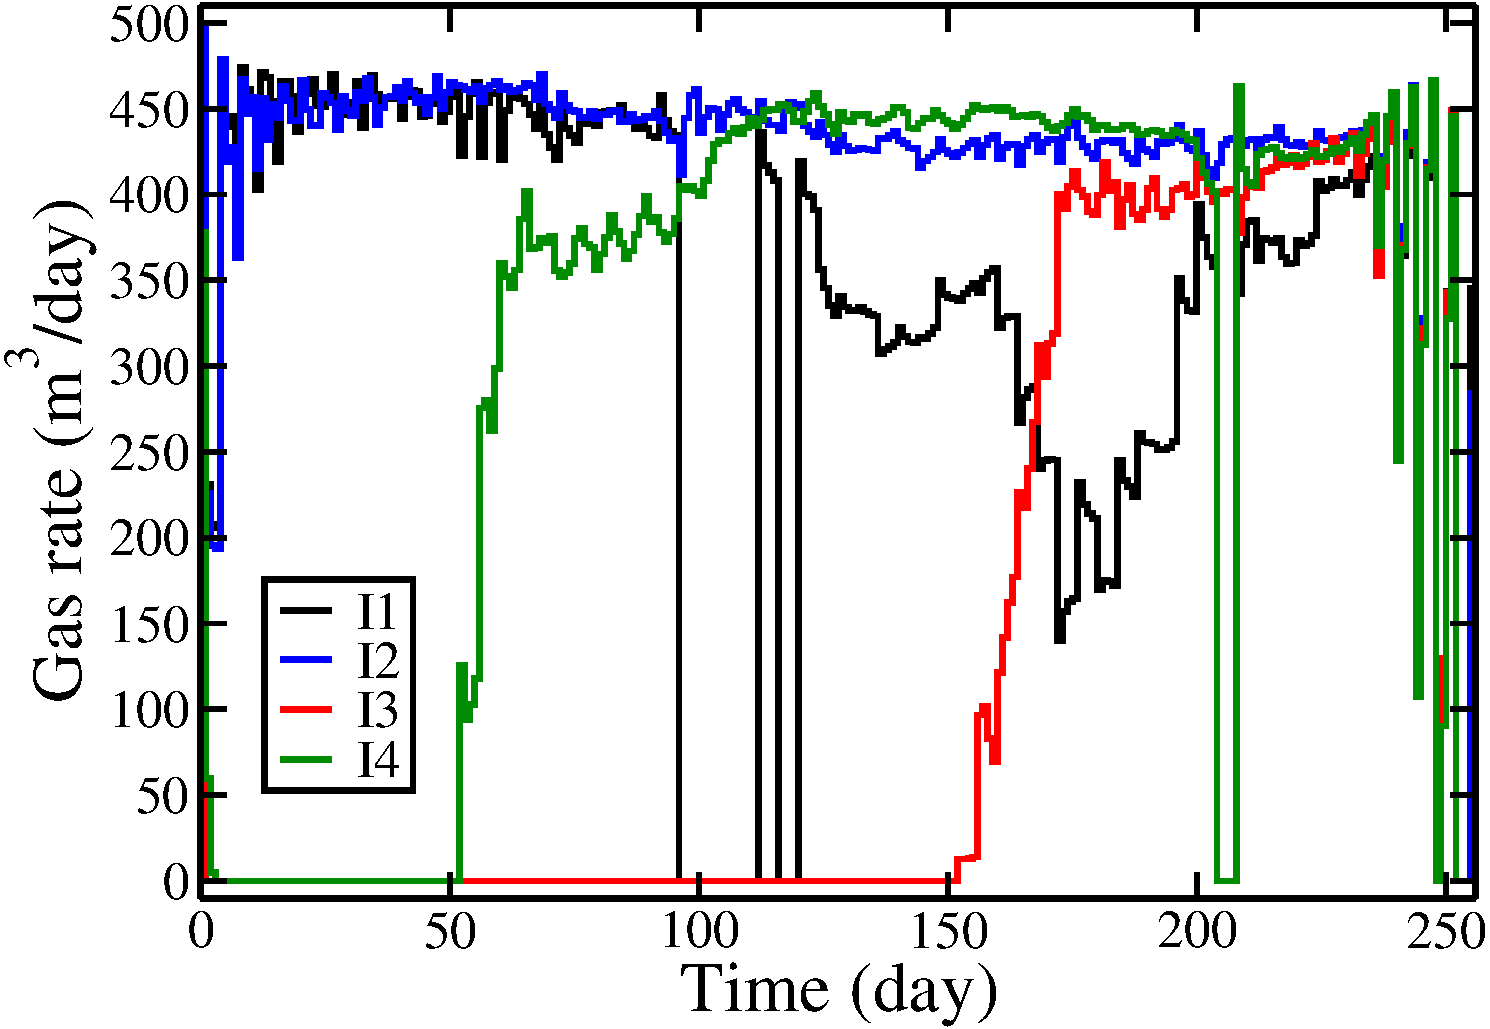
\includegraphics[totalheight=2.17in,angle=0]{FormalC600Steps64OptimalItPb_rate_gas.pdf}
%\end{center}
%\caption{BHPs (top) and gas rates (bottom) for the best formally constrained solution using 320 controls (Example 1, Run 7).}
%\label{fig:PIFormalControls320Plots}
%\end{figure}


%%%%%%%%%%%%%%%%%%%%%%%%%%%%%%%%%%%%%%%%%%%%%%%%%%%%%%%%%%%%%%%%%%%%%%%%%%%%






%%%%%%%%%%%%%%%%%%%%%%%%%%% Pi 1280 controls %%%%%%%%%%%%%%%%%%%%%%%%%%%%%%

%\begin{figure}
%\begin{center}
%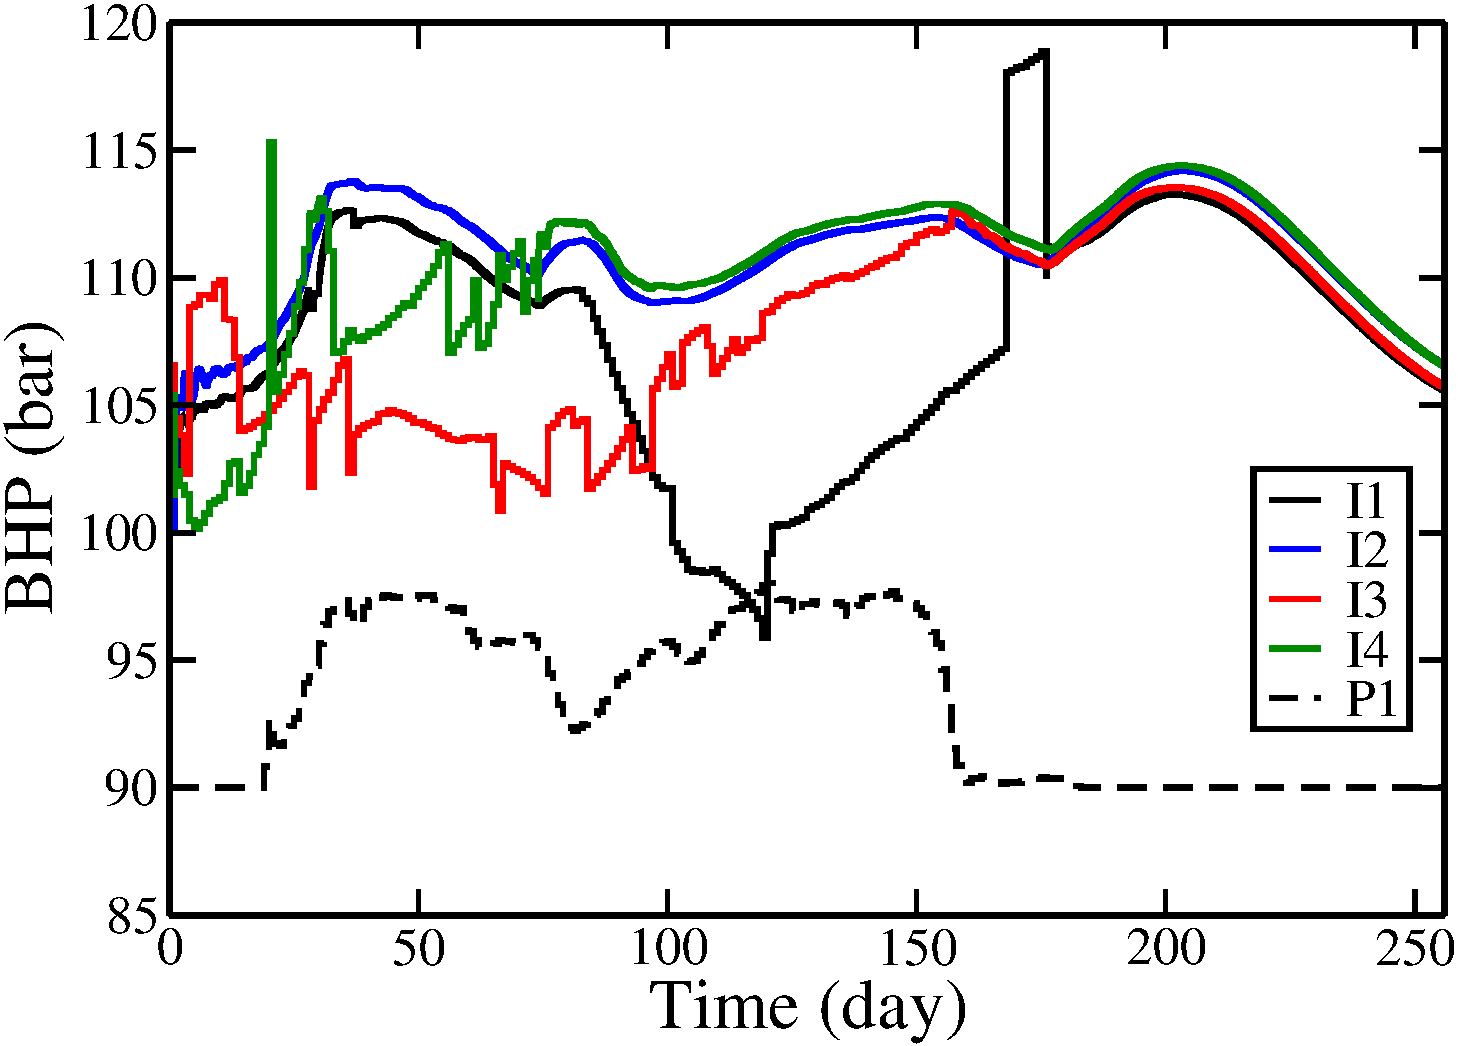
\includegraphics[totalheight=2.2in,angle=0]{OptimalC650HeuristicImPb_BHP.pdf}
%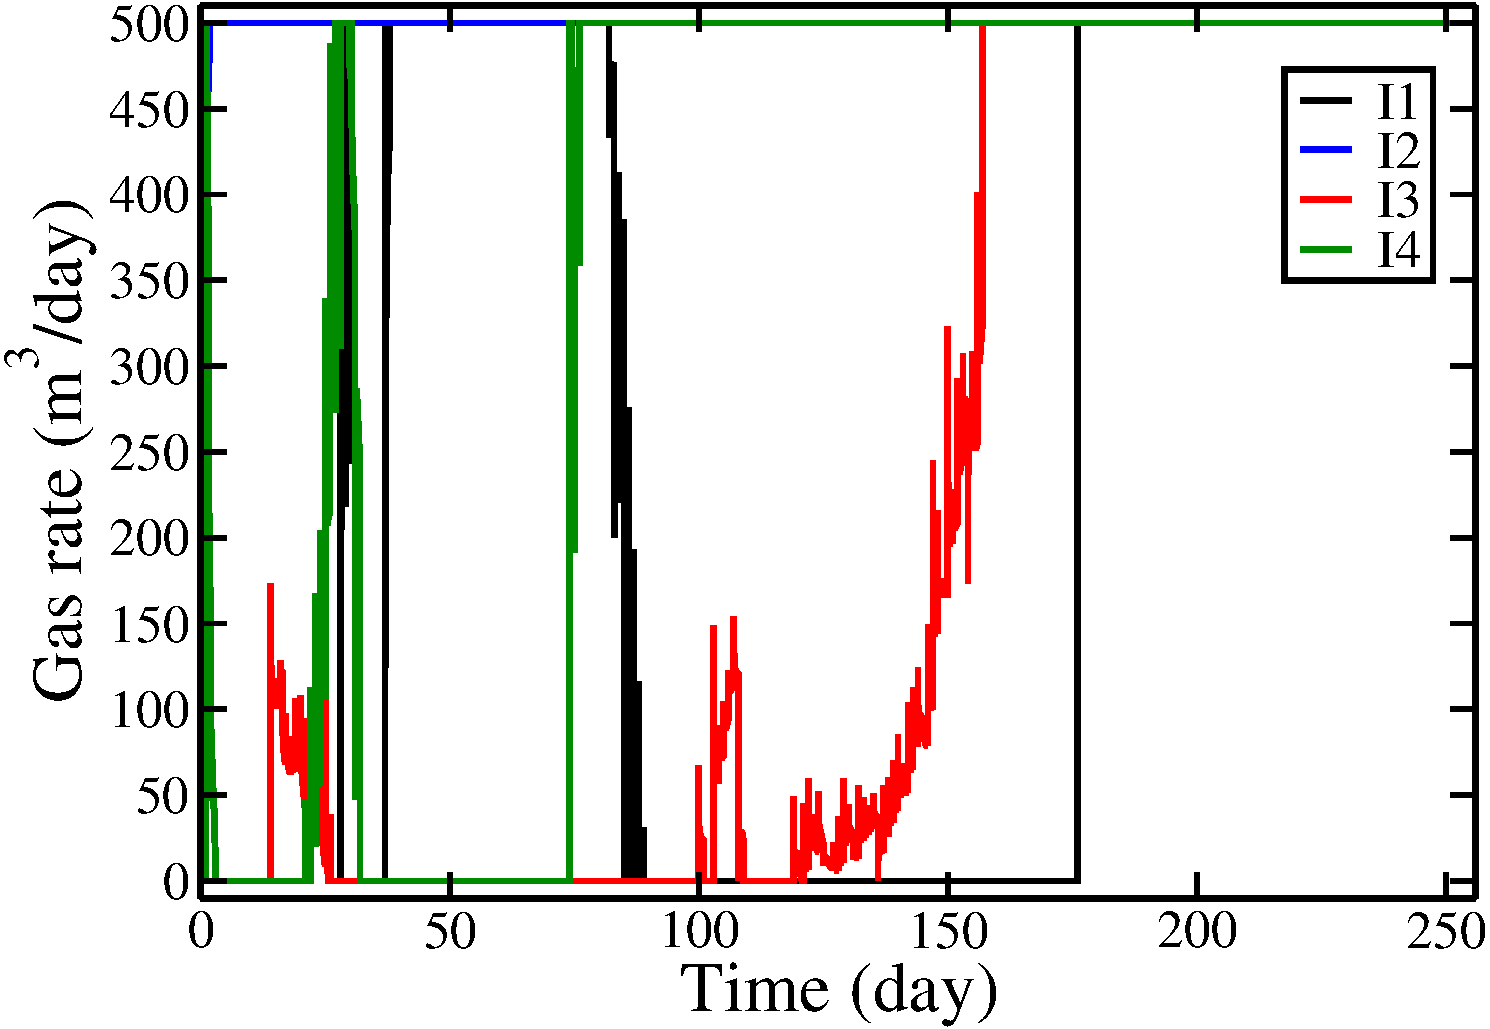
\includegraphics[totalheight=2.17in,angle=0]{OptimalC650HeuristicImPb_rate_gas.pdf}
%\end{center}
%\caption{BHPs (top) and gas rates (bottom) for the best heuristically constrained solution using 1280 controls (Example 1, Run 8).}
%\label{fig:PIHeuristicControls1280Plots}
%\end{figure}


%\begin{figure}
%\begin{center}
%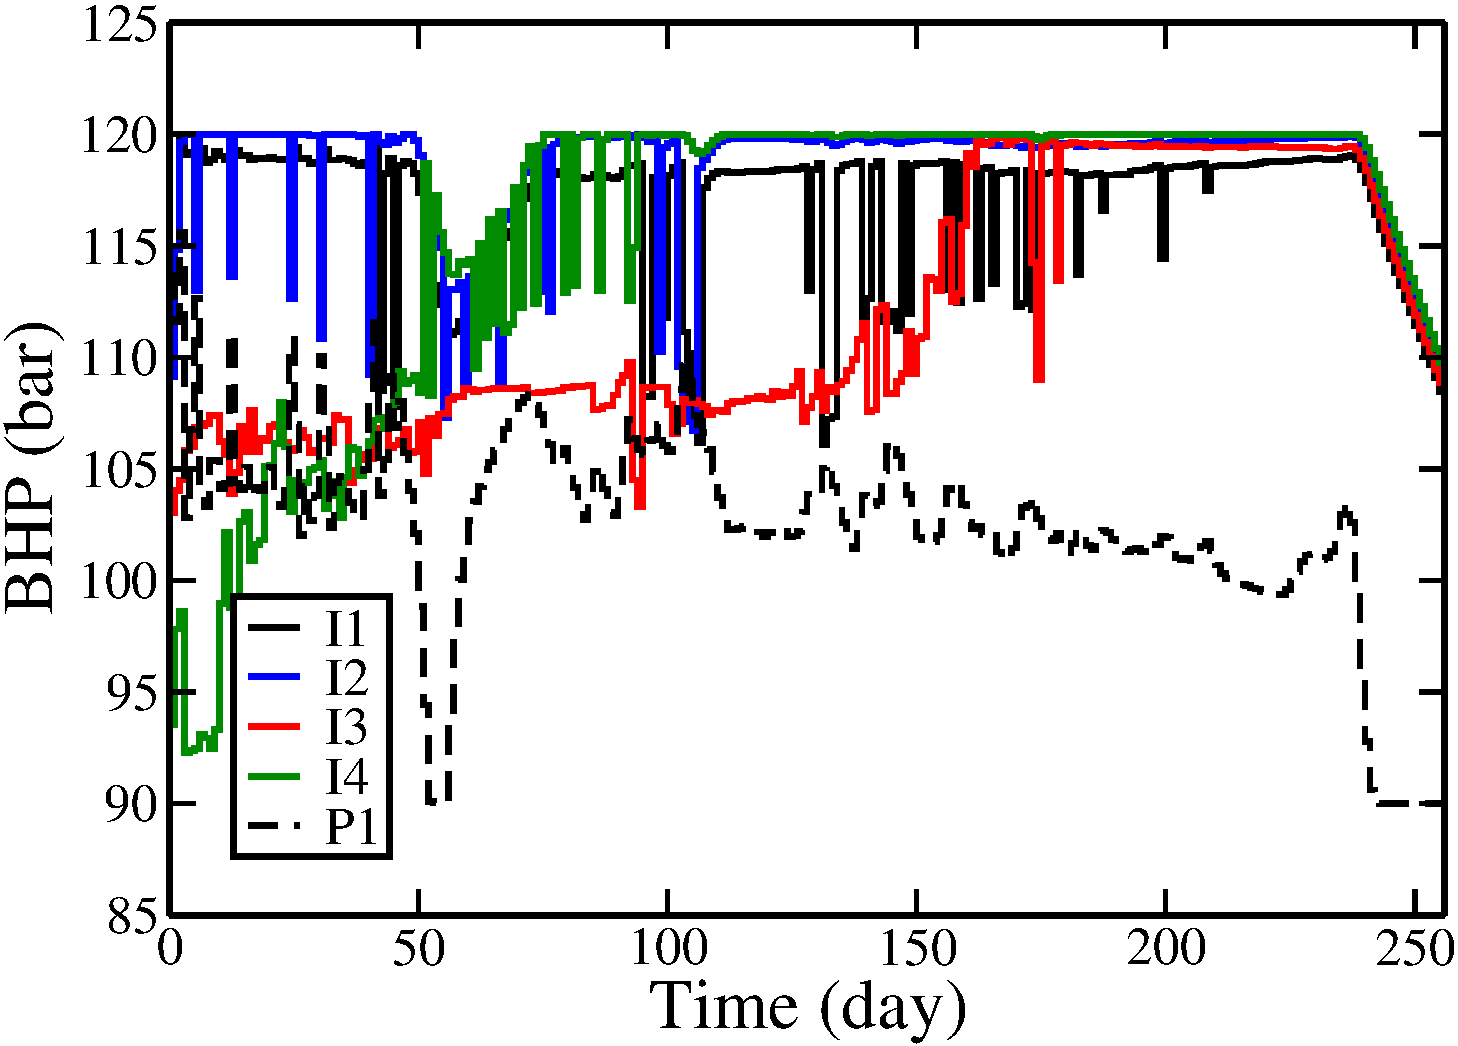
\includegraphics[totalheight=2.2in,angle=0]{OptimalC650OptimalImPm_BHP.pdf}
%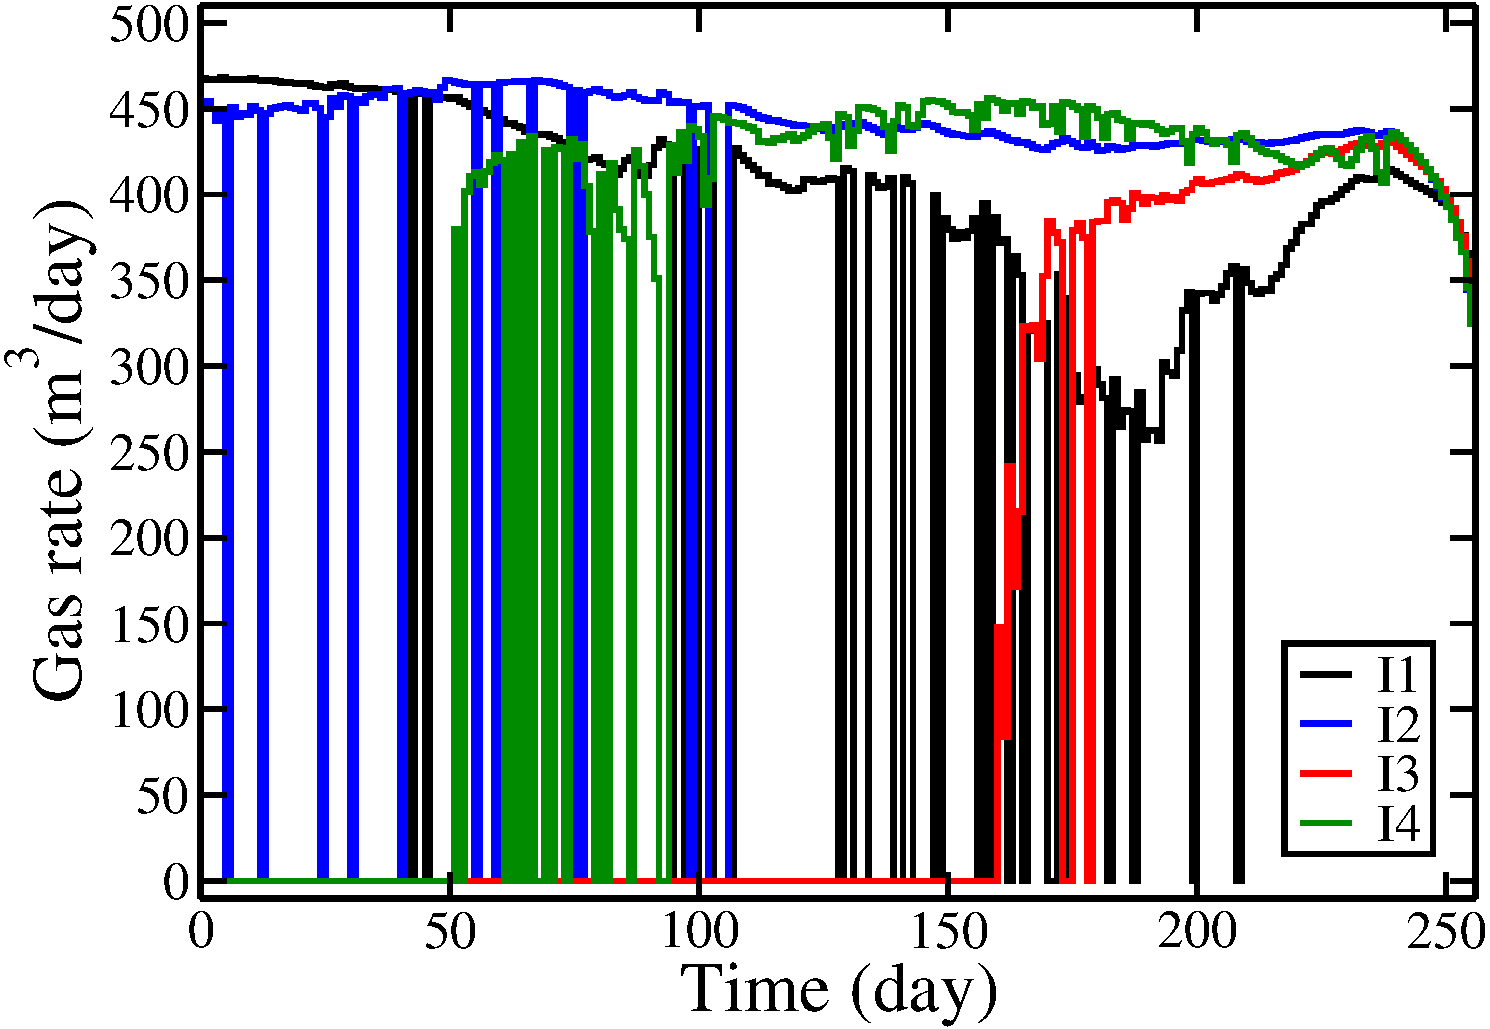
\includegraphics[totalheight=2.2in,angle=0]{OptimalC650OptimalImPm_rate_gas.pdf}
%\end{center}
%\caption{BHPs (top) and gas rates (bottom) for the best formally constrained solution using 1280 controls (Example 1, Run 4).}
%\label{fig:PIFormalControls1280Plots}
%\end{figure}

%%%%%%%%%%%%%%%%%%%%%%%%%%%%%%%%%%%%%%%%%%%%%%%%%%%%%%%%%%%%%%%%%%%%%%%%%%%%






\begin{figure}
\begin{center}
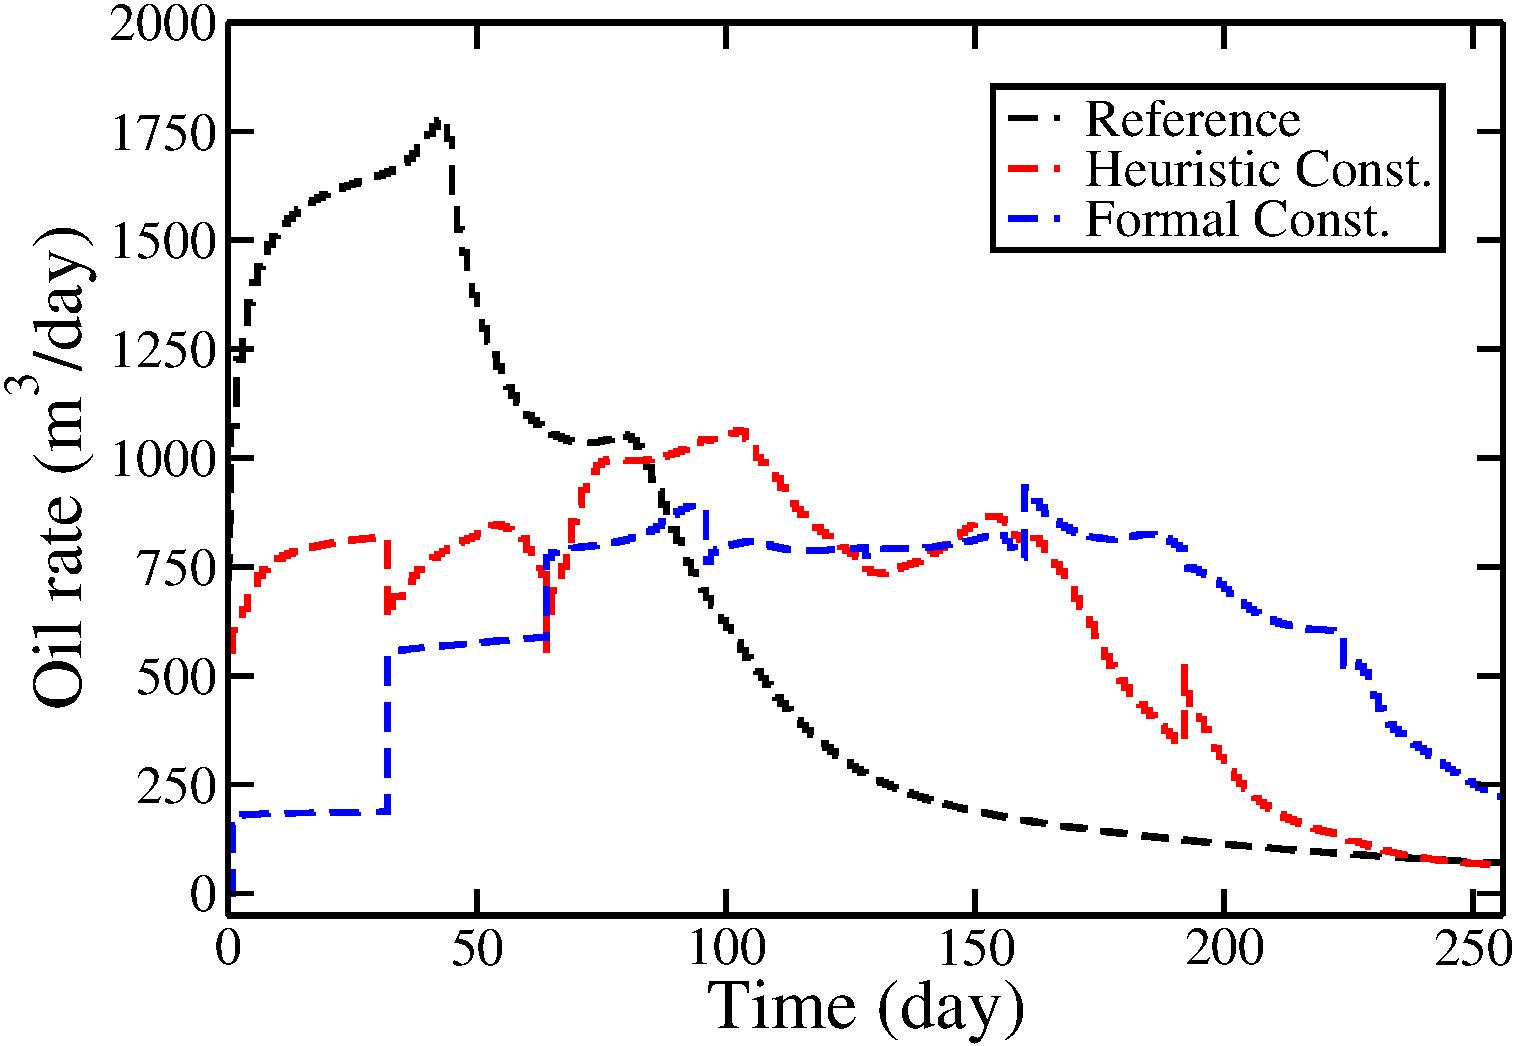
\includegraphics[totalheight=2.2in,angle=0]{OilRatesSteps8.pdf}
%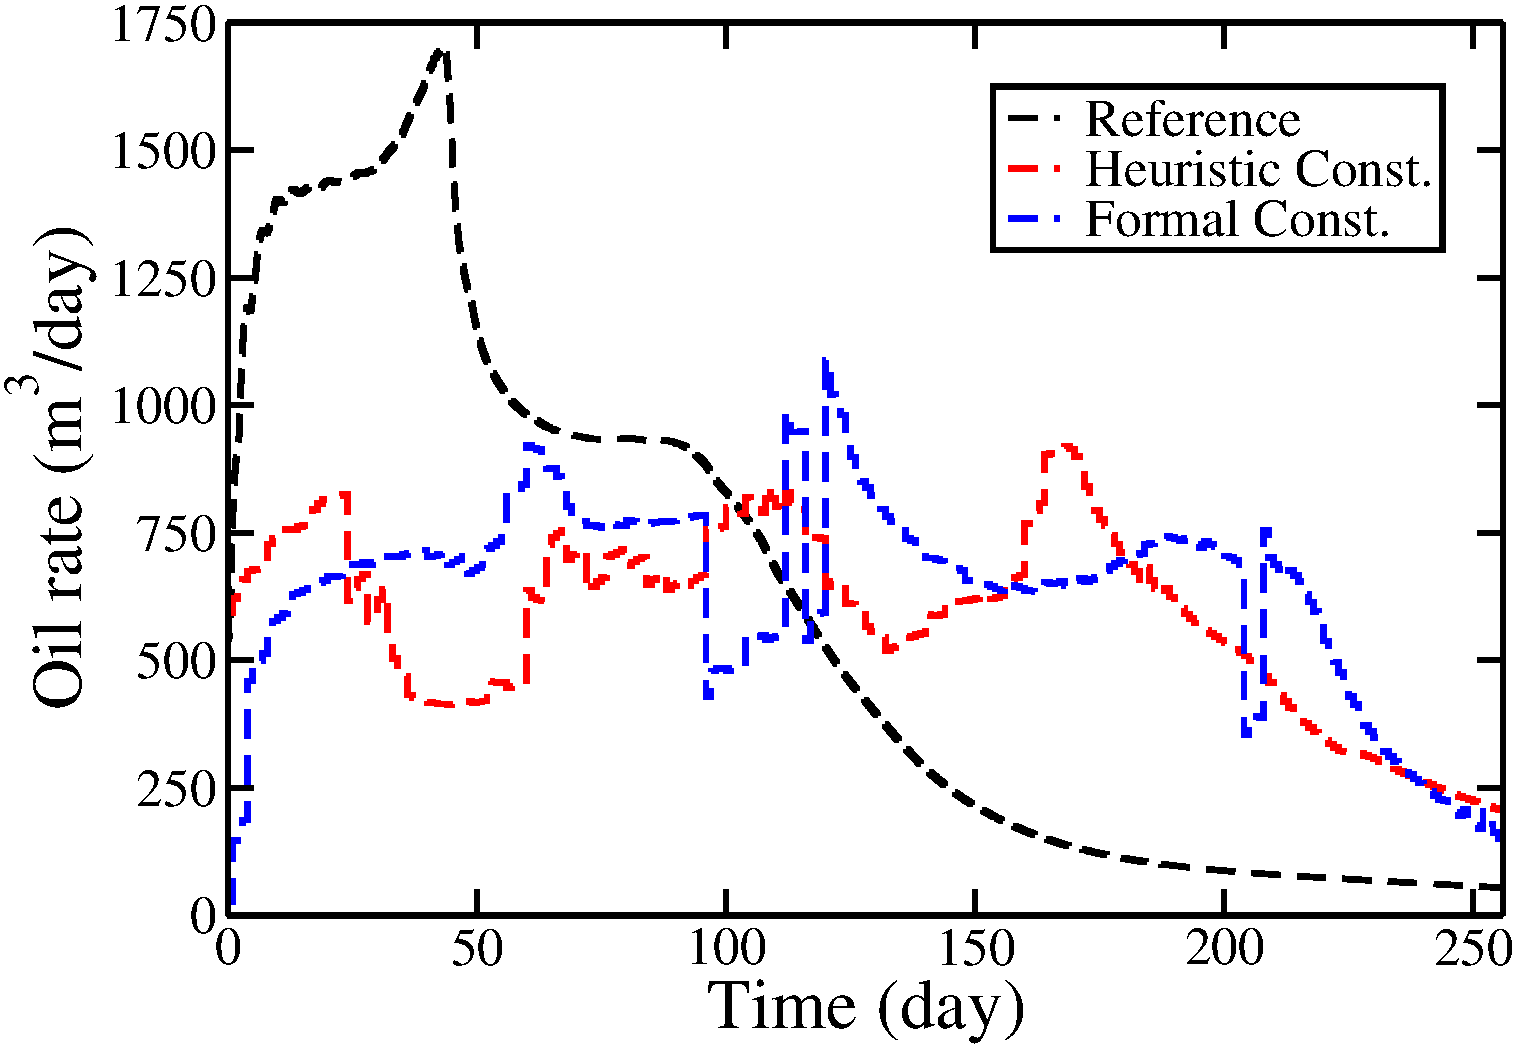
\includegraphics[totalheight=2.2in,angle=0]{OilRatesSteps64.pdf}
%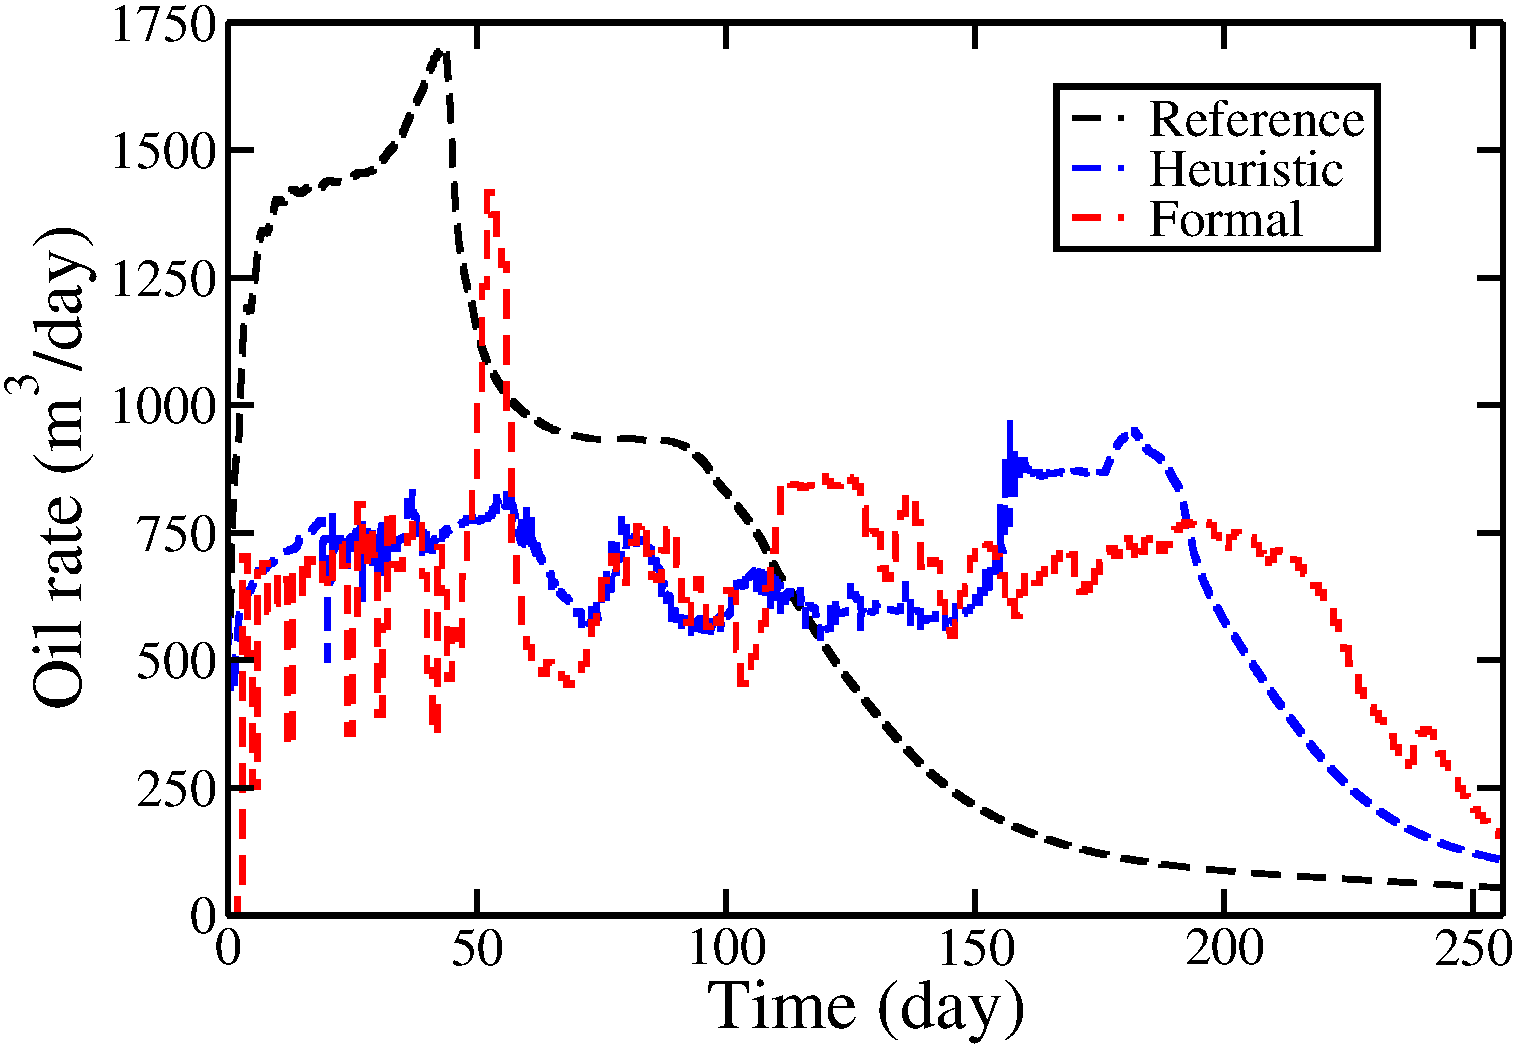
\includegraphics[totalheight=2.2in,angle=0]{OilRates.pdf}
\end{center}
\caption{Oil rates for Example 1 (40 controls), reference (black dashed line), heuristically constrained (red dashed line)
 and formally constrained (blue dashed line).} 
\label{fig:PIOilRates}
\end{figure}

%\begin{figure}
%\begin{center}
%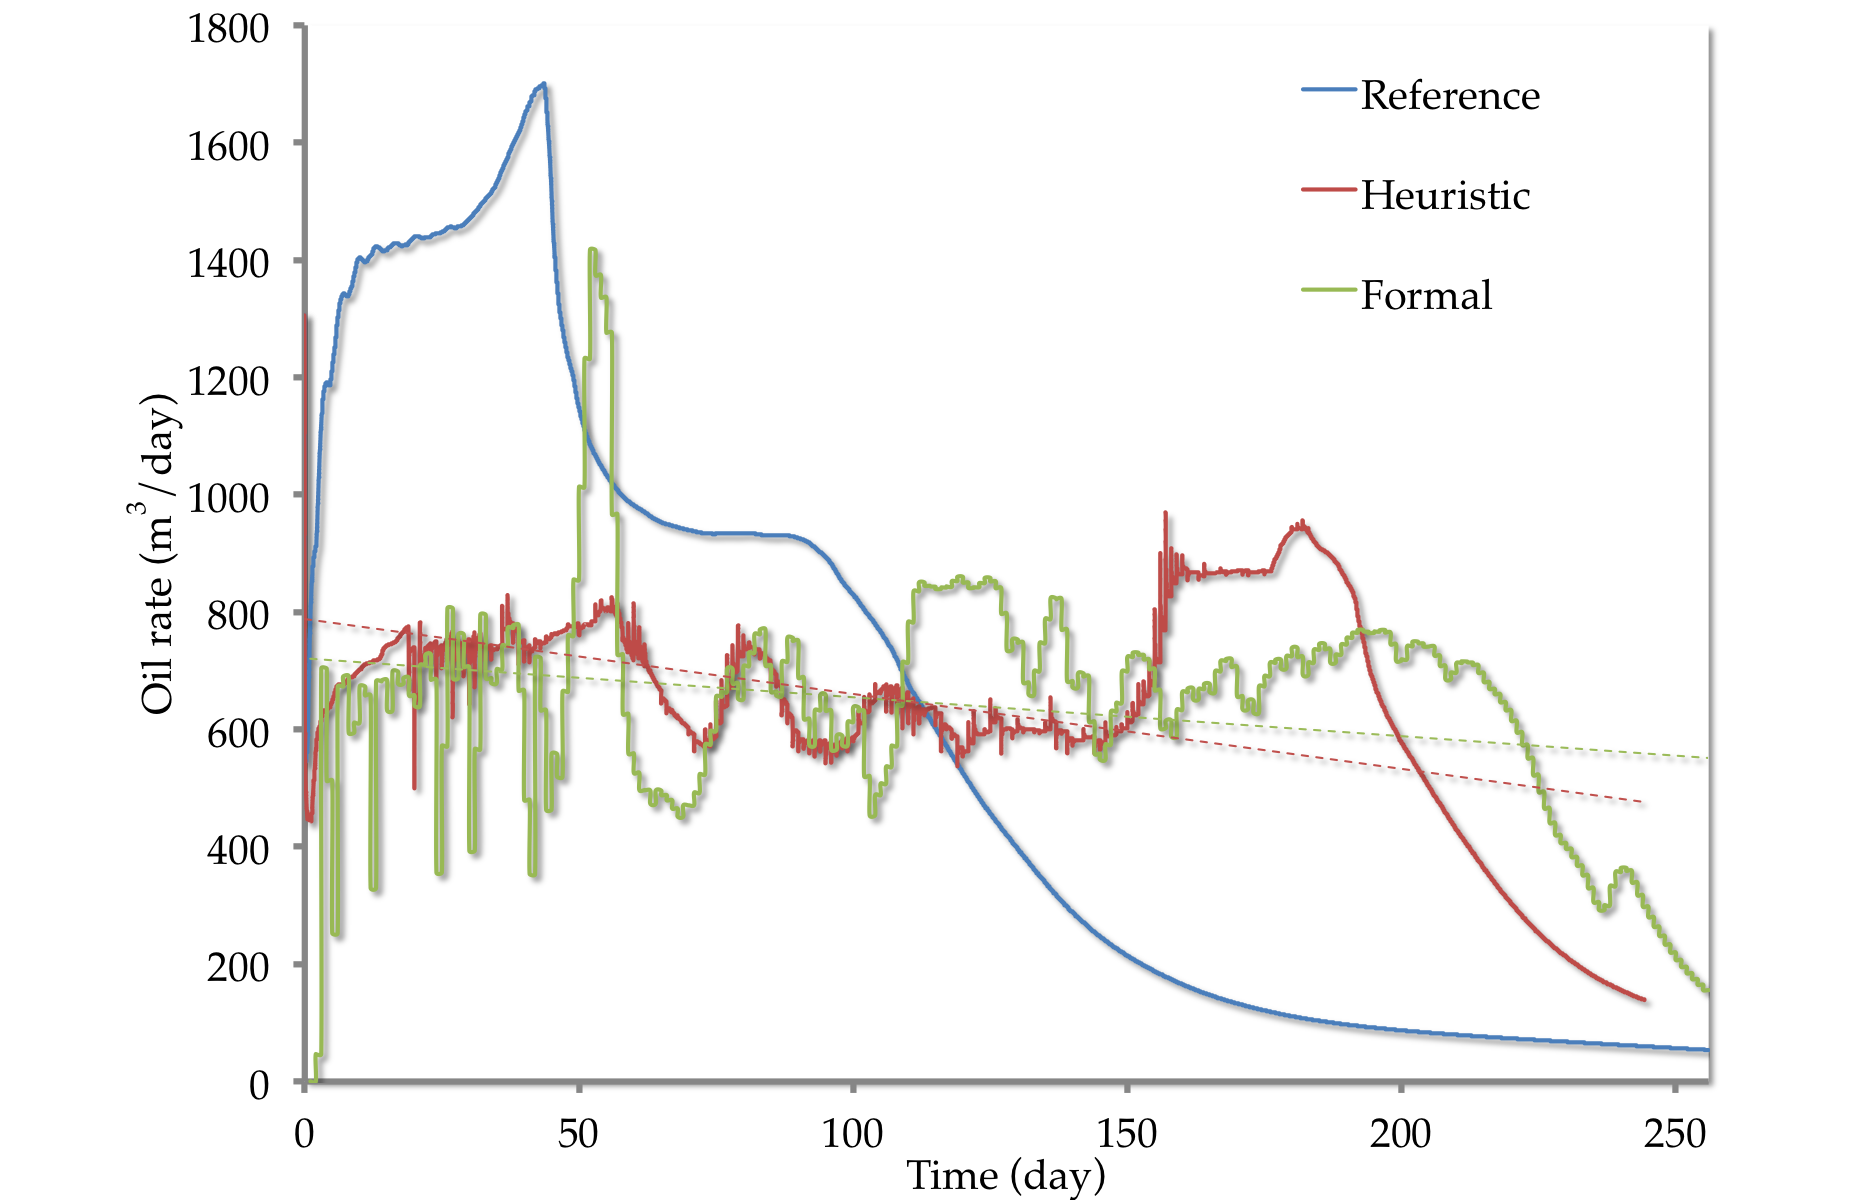
\includegraphics[totalheight=2.2in,angle=0]{OilRatesPiExcel.png}
%\end{center}
%\caption{Oil rates BHPs (top), gas rates (middle) and oil rates
%  (bottom) for the best formally constrained solution (Example 1, Run 8).}
%\label{fig:PIOilRatesExcel}
%\end{figure}
%





\subsection{Example 2 - Top layer of SPE 10 model}
%
In the second example we again maximize cumulative oil recovery under CO$_2$
injection. The two-dimensional geological model is the top layer of the model
defined in the SPE comparative solution project~\cite{Christie}, referred to as
SPE~10. The model includes a total of four components, as specified in
Table~\ref{table:fluidForSPE10TopLayer}. Details on the
reservoir model are provided in
Table~\ref{table:spe10toplayer}.

%
\begin{table}
\centering
\caption{Fluid description for Example 2}
\begin{tabular}{|l|r|r|r|r|}
\hline
%\multicolumn{5}{|c|}{SPE10 top layer}    \\
%\hline
Component            & CO$_2$ & C$_1$ & C$_4$ & C$_{10}$    \\
\hline
Initial composition (\%)  & 1    & 20  & 29    & 50 \\
Injection composition (\%)& 90   & 10 & - & - \\
\hline
\end{tabular}
\label{table:fluidForSPE10TopLayer}
\end{table}
%


\begin{table}
\centering
\caption{Model parameters for Example 2}
\begin{tabular}{|l|rr|}
\hline
%\multicolumn{3}{|c|}{SPE10 top layer}  \\
%\hline
Grid size                & 60 $\times$ 220 $\times$ 1 &       \\
\hline\hline
Parameter                & Value    & Units \\
\hline
$\Delta x$               & 6.096&m          \\
$\Delta y$               & 3.048&m          \\
$\Delta z$               & 0.6096&m         \\
Depth                    & 2574&m           \\
Initial pressure         & 75  & bar        \\
Temperature              &$100$ & $^\circ$C     \\
\hline
Rock compressibility     & $7.2 \times 10^{-5}$ & 1 / bar \\
Simulation time          &1000 & d          \\
Pressure upper bound     & 150 & bar        \\
Pressure lower bound     &  50 & bar        \\
\hline
Residual gas saturation  & 0 & -            \\
Residual oil saturation  & 0 & -            \\
End point rel perm gas   & 1 & -            \\
End point rel perm oil   & 1 & -            \\
Corey exponent gas       & 2 & -            \\
Corey exponent oil       & 2 & -            \\
\hline\hline
Well locations [grid block no.] & $i$ & $j$     \\
\hline
Injector 1               &   58&   9   \\
Injector 2               &   58& 126   \\
Injector 3               &    2&  67   \\
Injector 4               &    2& 211   \\
Producer 1               &    2&   3   \\
Producer 2               &   58&  67   \\
Producer 3               &    2& 143   \\
Producer 4               &   58& 210   \\
\hline
\end{tabular}
\label{table:spe10toplayer}
\end{table}



The well locations, along with a map of the permeability field, are depicted in
Fig.~\ref{fig:PermeabilityMapAndWellsSpe10Top}. The control parameters in the
optimization problem are again well BHPs, constrained to lie between 150~bar and 50~bar. A
maximum (per well) gas production rate of 200~m$^3/$d at reservoir conditions is also specified.
The total simulation period is 1000~days. The well controls are determined
at initial time and then at every 100-day interval. There are a
total of ten control steps and 80 control parameters in this example.


%
\begin{figure}[ht]
\begin{center}
     \begin{tabular}{cccccccc}
      0.003 &  0.023 & 0.178 & 1.358 & 10.38 & 79.43 & 607.6 &4648
      \end{tabular}
      
\includegraphics[width=8cm, height=0.5cm]{VanEssenModelPermeabilityMapColorBar.png}
       
       \medskip

       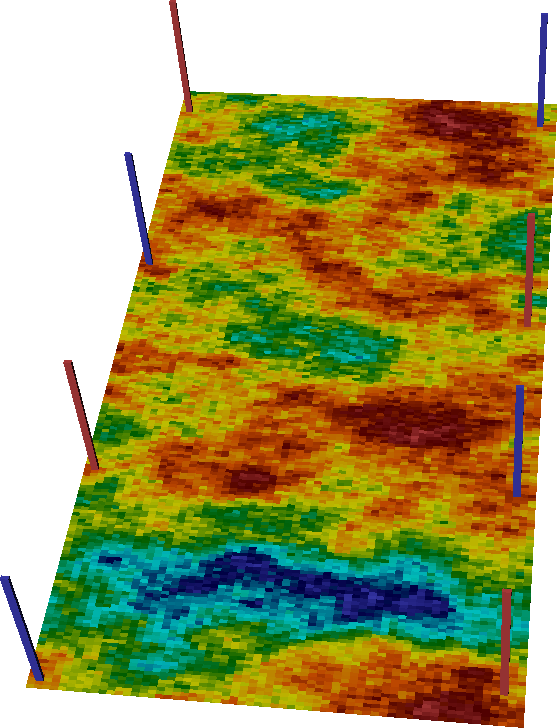
\includegraphics[totalheight=3.2in]{SPE10TopModelPermeabilityMapConstantRotated.png} %SPE10TopPermeabilityMapAndWells.png}

        %\medskip

       %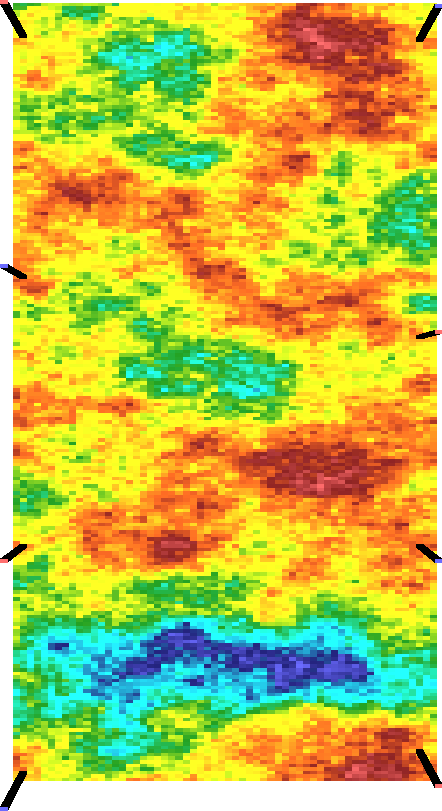
\includegraphics[totalheight=3.2in, angle=270]{SPE10TopModelPermeabilityMapConstant.png} %SPE10TopPermeabilityMapAndWells.png}
\end{center}
     \caption{Injection wells (blue) and production wells (red) for Example 2. Background shows $\log \tens{K}_x$ ($ \tens{K}_x = \tens{K}_y$).}
  \label{fig:PermeabilityMapAndWellsSpe10Top}
\end{figure}
%

\begin{table}
\centering
\caption{Oil production in $10^3$~m$^3$ (Example 2) for the optimized objective function
         without satisfying the nonlinear constraints (`Unconstr.'), satisfying the nonlinear constraints
         using the heuristic treatment (`Heuristic'), and satisfying the nonlinear constraints
         using the formal approach (`Formal'). Best feasible results shown in bold.}
\begin{tabular}{|c|c|c|c|}
\hline
  Run            &  Unconstr. & Heuristic & Formal      \\
\hline
Reference        & 20.29         &     20.28         & 	         \\
1 & 21.77      &     21.77         &       21.77    \\
2 & 22.01      &     22.01         &       22.01    \\
3 & 18.16      &     18.16         &       18.17    \\
4 & 21.68      &     21.68         &       21.68    \\
5 & 22.03      & \bf{22.03}      &       22.04    \\
6 & 22.13      &     20.67         &  \bf{22.20}    \\
7 & 21.68      &     21.68         &       21.99    \\
8 & 22.07      &     21.48         &       22.07    \\
9 & 22.03      & \bf{22.03}      &       22.03    \\
\hline
\end{tabular}
  \label{table:spe10top}
\end{table}

%1 & O25G16     &     21400         &       O78G57 \\
%2 & O25G16     & \bf{21980}        &       O46G35 \\
%3 & O48G34     &     16800         &       O31G22 \\
%4 & O25G17     &     21600         &       O79G46 \\
%5 & O21G17     &     19900         &       O140G62\\
%6 & O28G15     &     19800         &       O41G32 \\
%7 & O24G15     &     21000         &       O77G61 \\
%8 & O21G14     &     20500         &       O67G49 \\
%9 & O29G19     &     20900         &       O77G49 \\


We first generate two reference solutions as in the previous example. The cumulative oil production for these two cases, given in the first row (`Reference') of Table~\ref{table:spe10top}, are nearly identical because the nonlinear constraint violation in the
unconstrained case is small. We next perform (nine) optimizations that honor the bound constraints but not the nonlinear constraints. The best optimum achieved in this case provides a cumulative oil production of 22,130~m$^3$ (Run~6). Using the heuristic constraint handling procedure (third column), the best result is 22,030~m$^3$ of oil (Runs~5 and 9), which
exceeds the reference heuristic result by 8.8\%. The best optimum achieved using the formal constraint handling treatment is 22,200~m$^3$ of oil (Run~6). This value exceeds the reference solution by 9.5\% and the best result using the heuristic treatment by 0.8\%. It also exceeds the best unconstrained result (again, unconstrained here refers to the nonlinear constraints) of 22,130~m$^3$, which is presumably because the nonlinear constraints are not important in this example.

Oil production profiles are shown in Fig.~\ref{fig:SPE10TopLayerRevenue}. These profiles are very similar for the runs using the heuristic and formal constraint handling procedures. The BHP, gas rate, and oil rate profiles for the three cases are shown in
Figs.~\ref{fig:SPE10TopLayerReferenceRates},
\ref{fig:SPE10TopLayerUnconstrainedOptimalChoppedRates} and
\ref{fig:SPE10TopLayerConstrainedOptimalRates}. We see that the gas production rates satisfy the nonlinear constraints (200~m$^3/$d) at all times for both constraint handling procedures. Consistent with Fig.~\ref{fig:SPE10TopLayerRevenue}, the oil production rates in Figs.~\ref{fig:SPE10TopLayerUnconstrainedOptimalChoppedRates} and
\ref{fig:SPE10TopLayerConstrainedOptimalRates} resemble one another, and they are significantly different than the reference solution in Fig.~\ref{fig:SPE10TopLayerReferenceRates}. For this example, the formal approach again required about three times the number of forward
simulations as the heuristically constrained approach.


\begin{figure} [ht]
\begin{center}
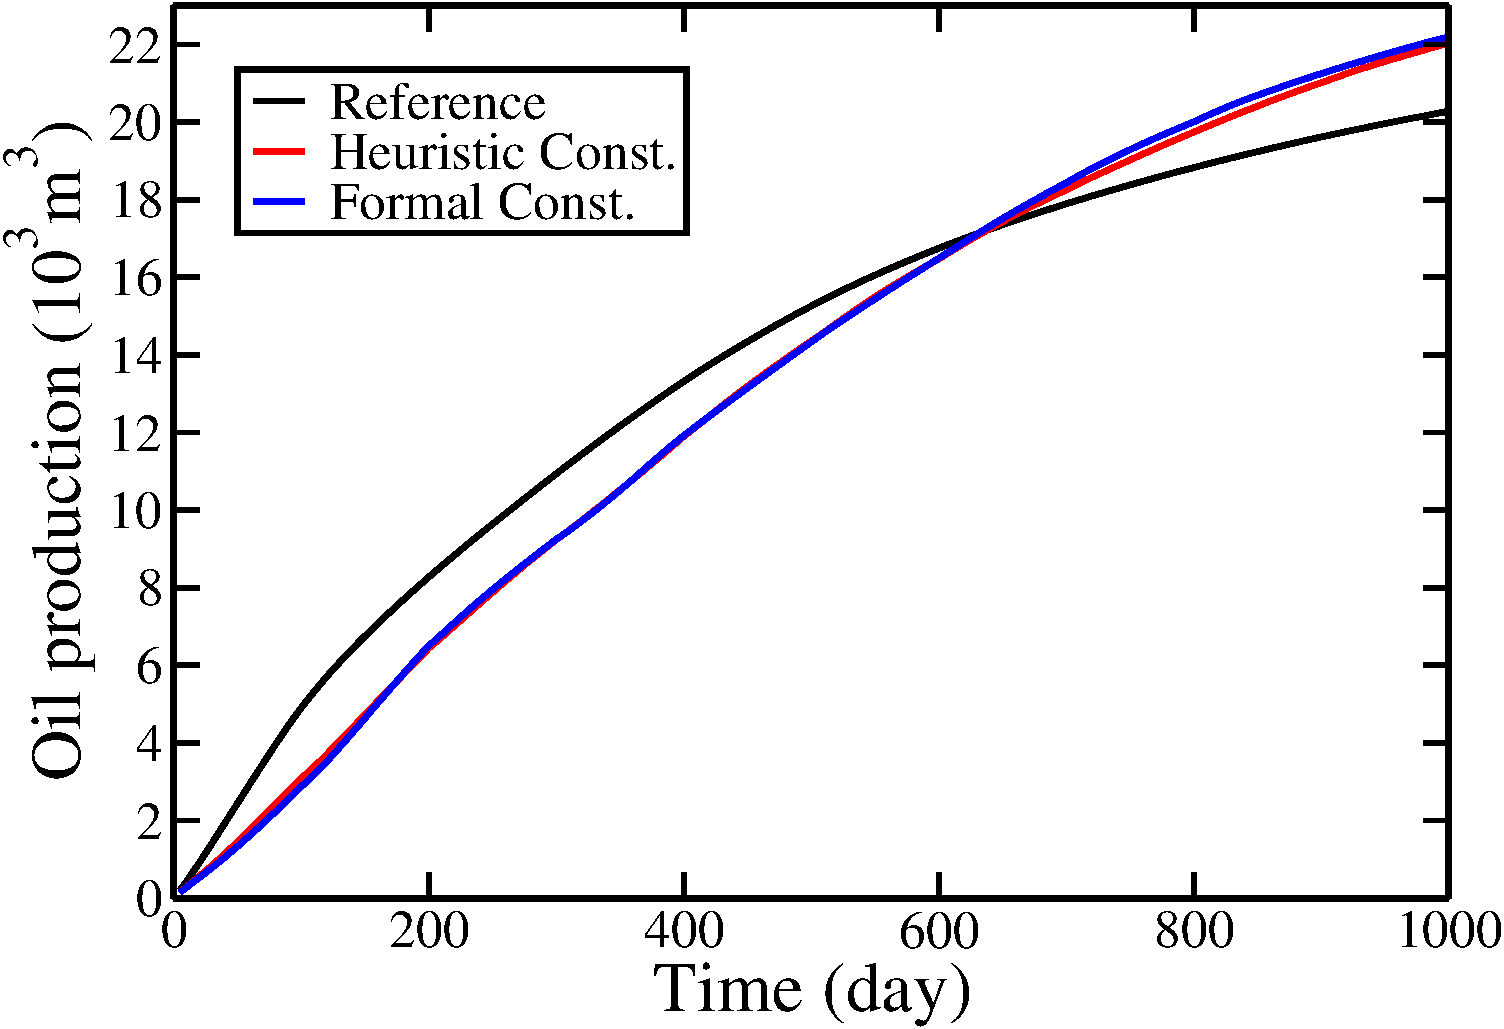
\includegraphics[totalheight=2.17in,angle=0]{spe10TopLayerRevenue.pdf}
\end{center}
\caption{Oil production versus time for Example 2. Results are for
  feasible reference case (black curve), best heuristically constrained solution (Run~9, red curve)
  and best formally constrained solution (Run~6, blue curve).}
\label{fig:SPE10TopLayerRevenue}
\end{figure}
\begin{figure}
\begin{center}
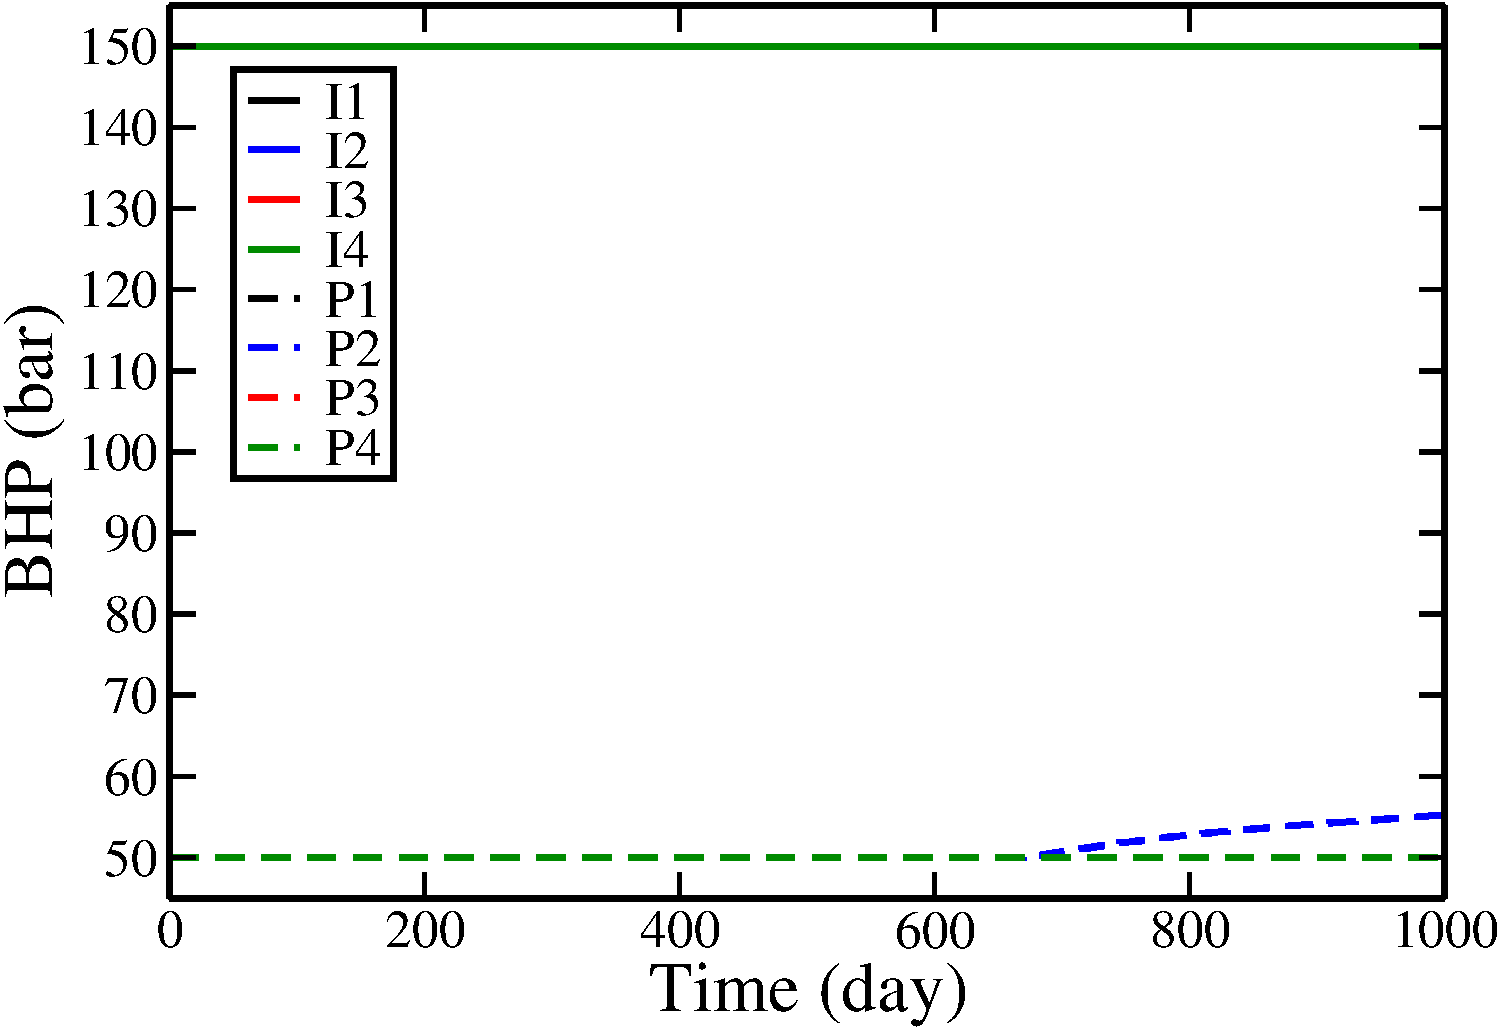
\includegraphics[totalheight=2.2in,angle=0]{spe10topLayerReferenceC200_BHP.pdf}
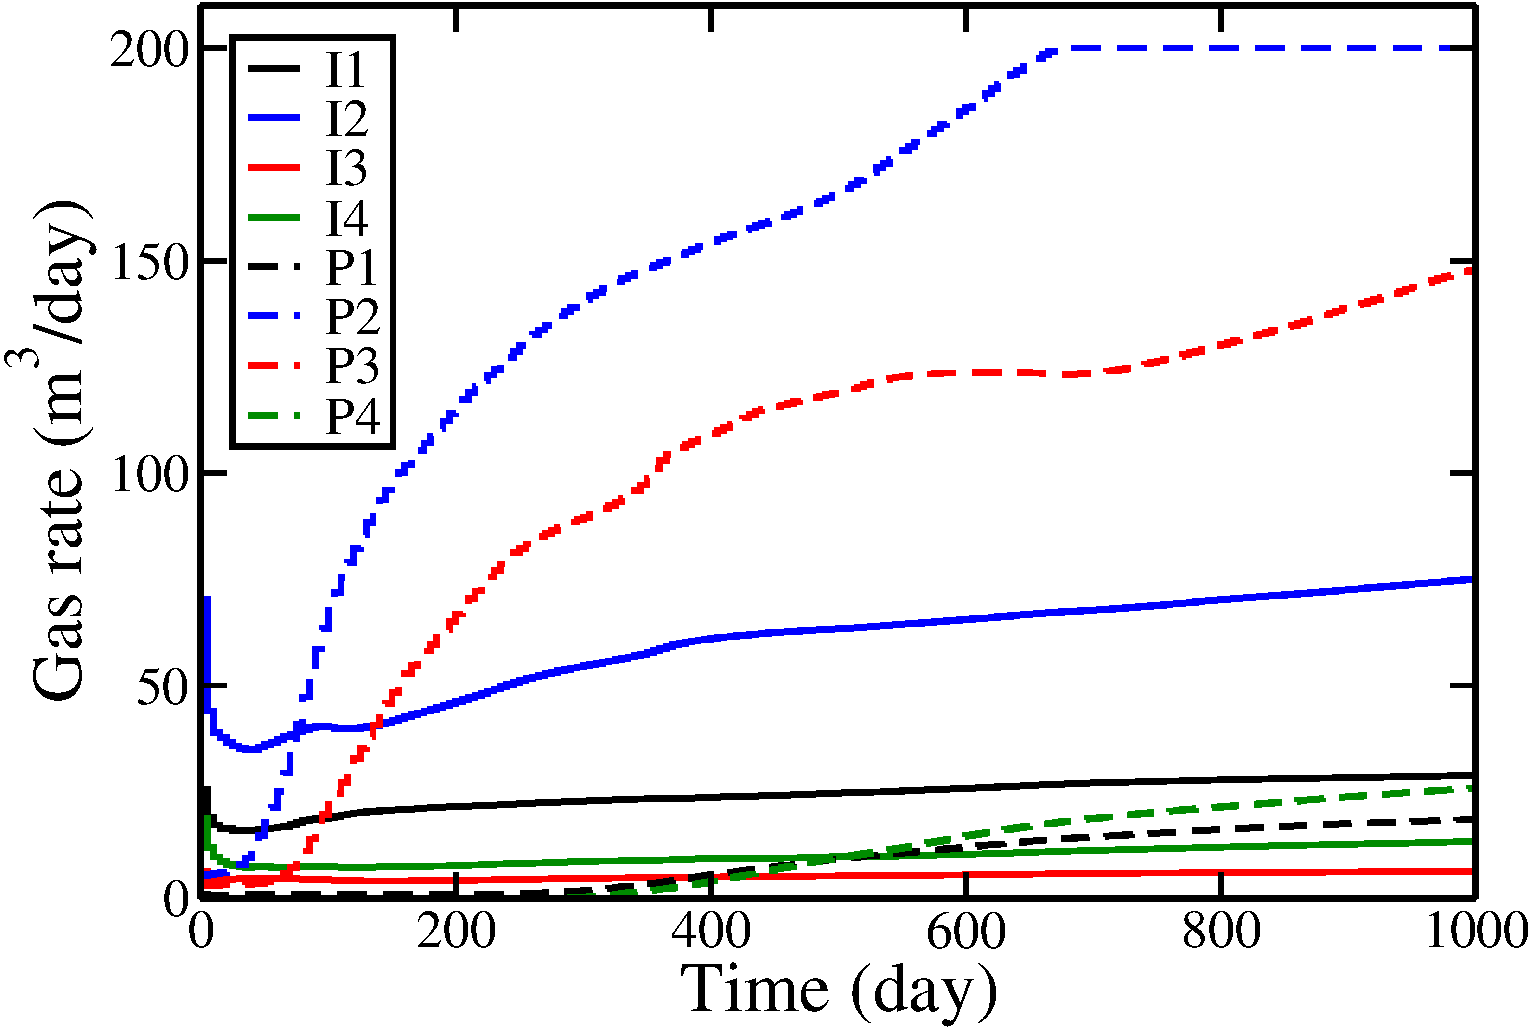
\includegraphics[totalheight=2.17in,angle=0]{spe10topLayerReferenceC200_rate_gas.pdf}
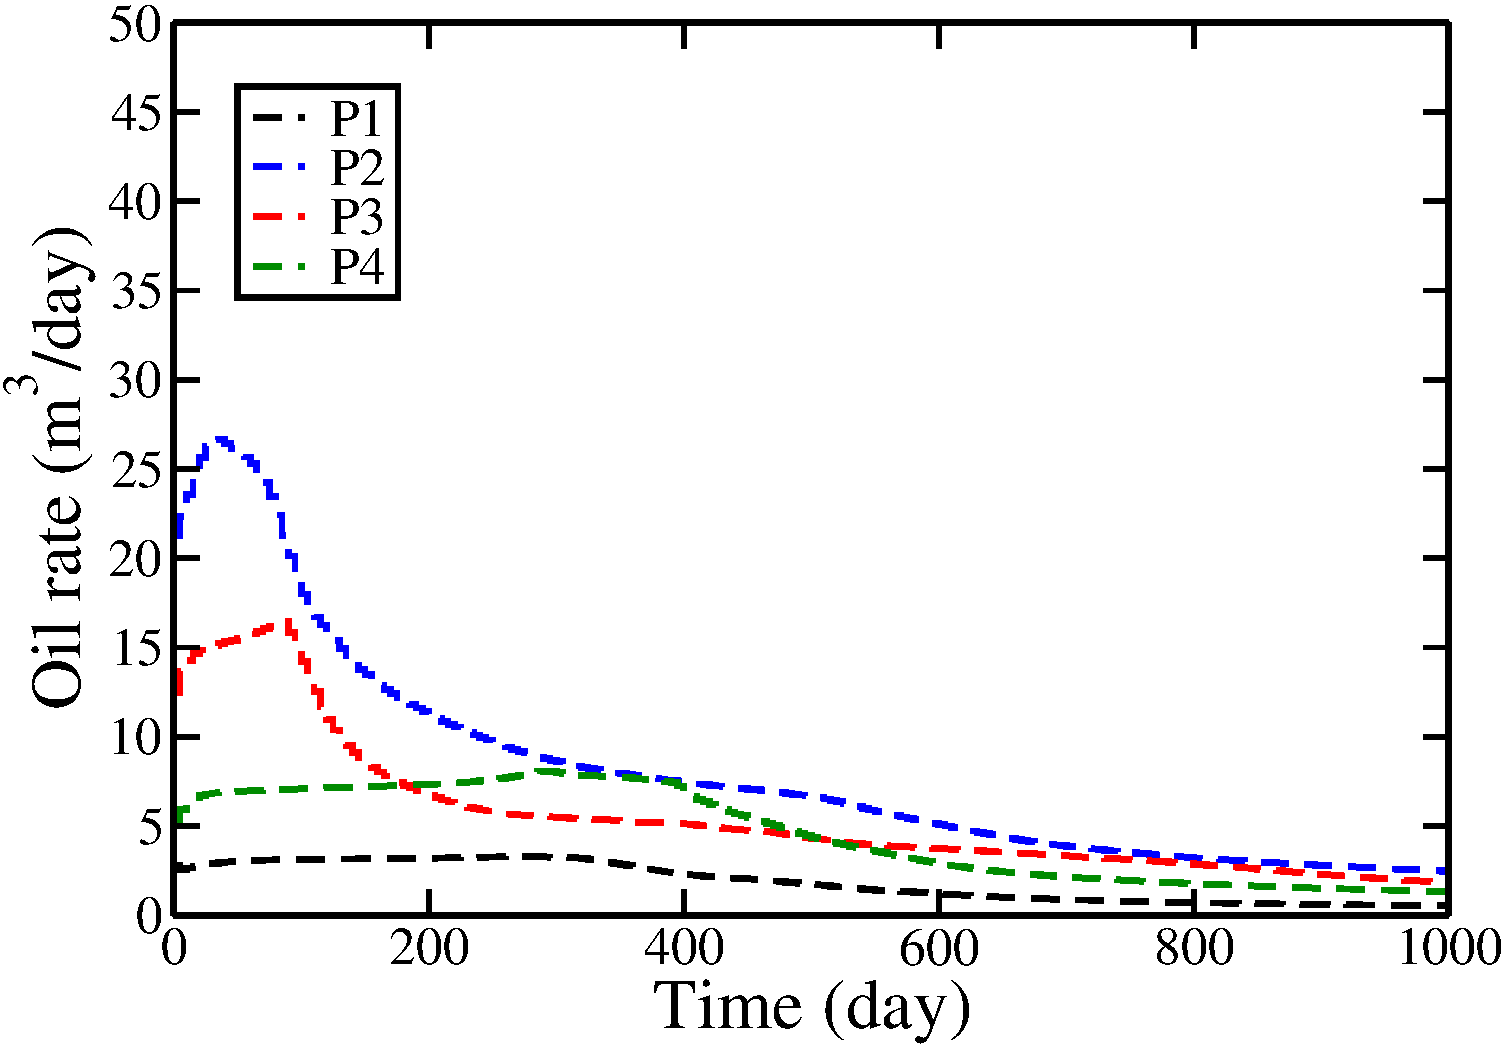
\includegraphics[totalheight=2.2in,angle=0]{spe10topLayerReferenceC200_rate_oil.pdf}
\end{center}
\caption{BHPs (top), gas rates (middle) and oil rates
  (bottom) for the feasible reference solution (Example 2).}
\label{fig:SPE10TopLayerReferenceRates}
\end{figure}

\begin{figure}
\begin{center}
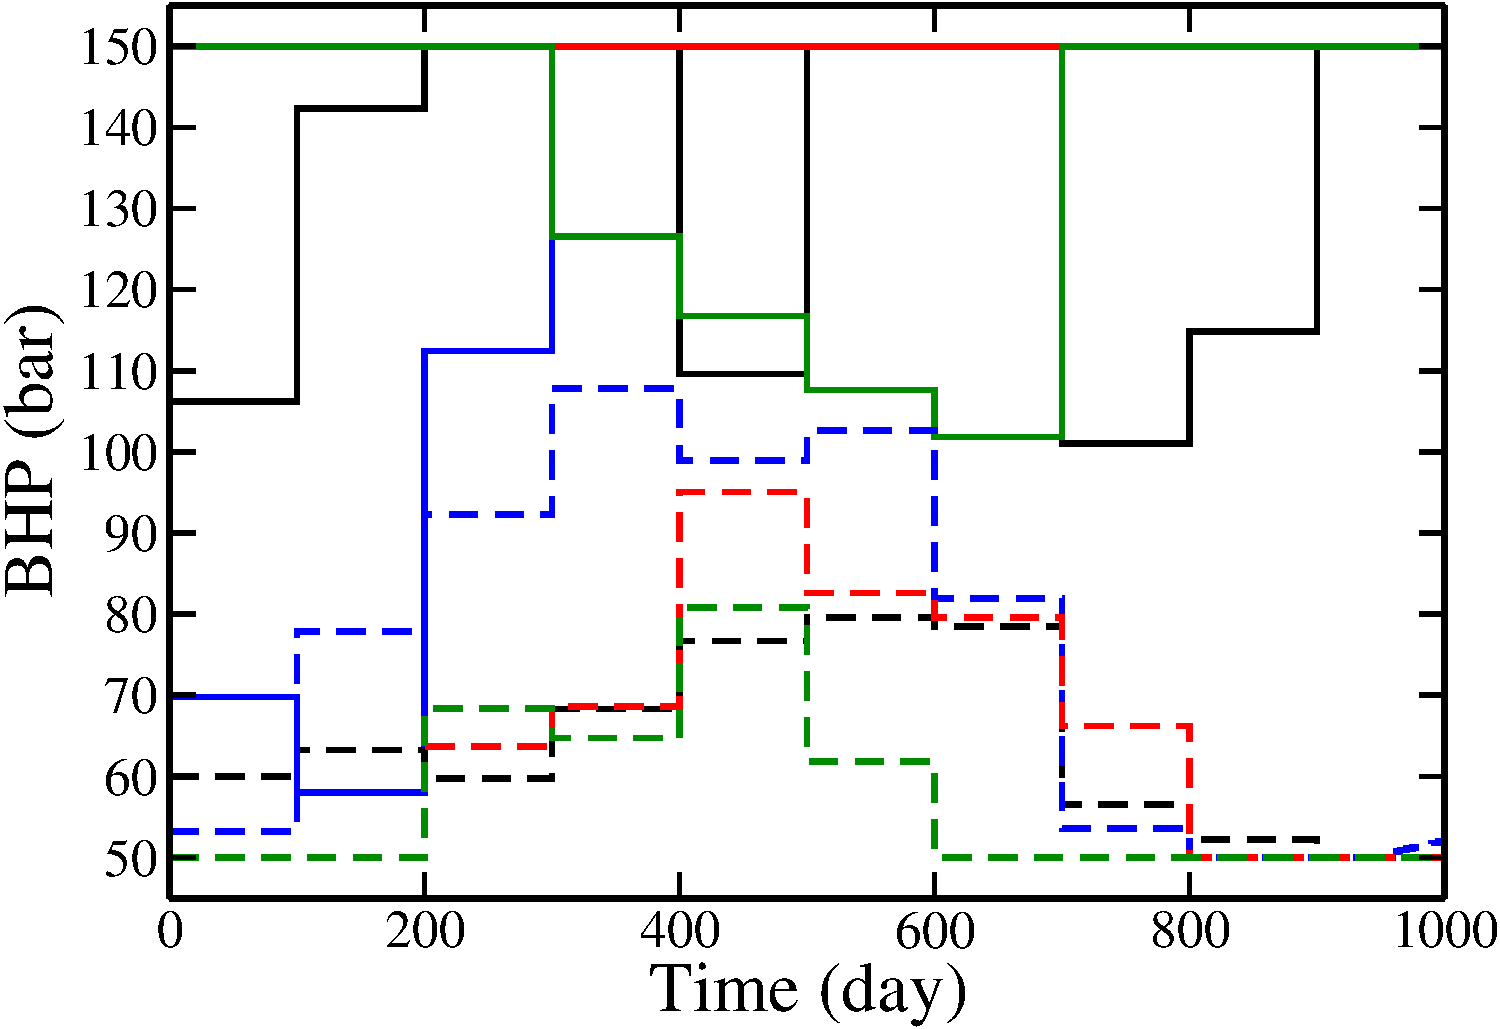
\includegraphics[totalheight=2.2in,angle=0]{spe10topLayerOptimalChoppedIuPu_BHP.pdf}
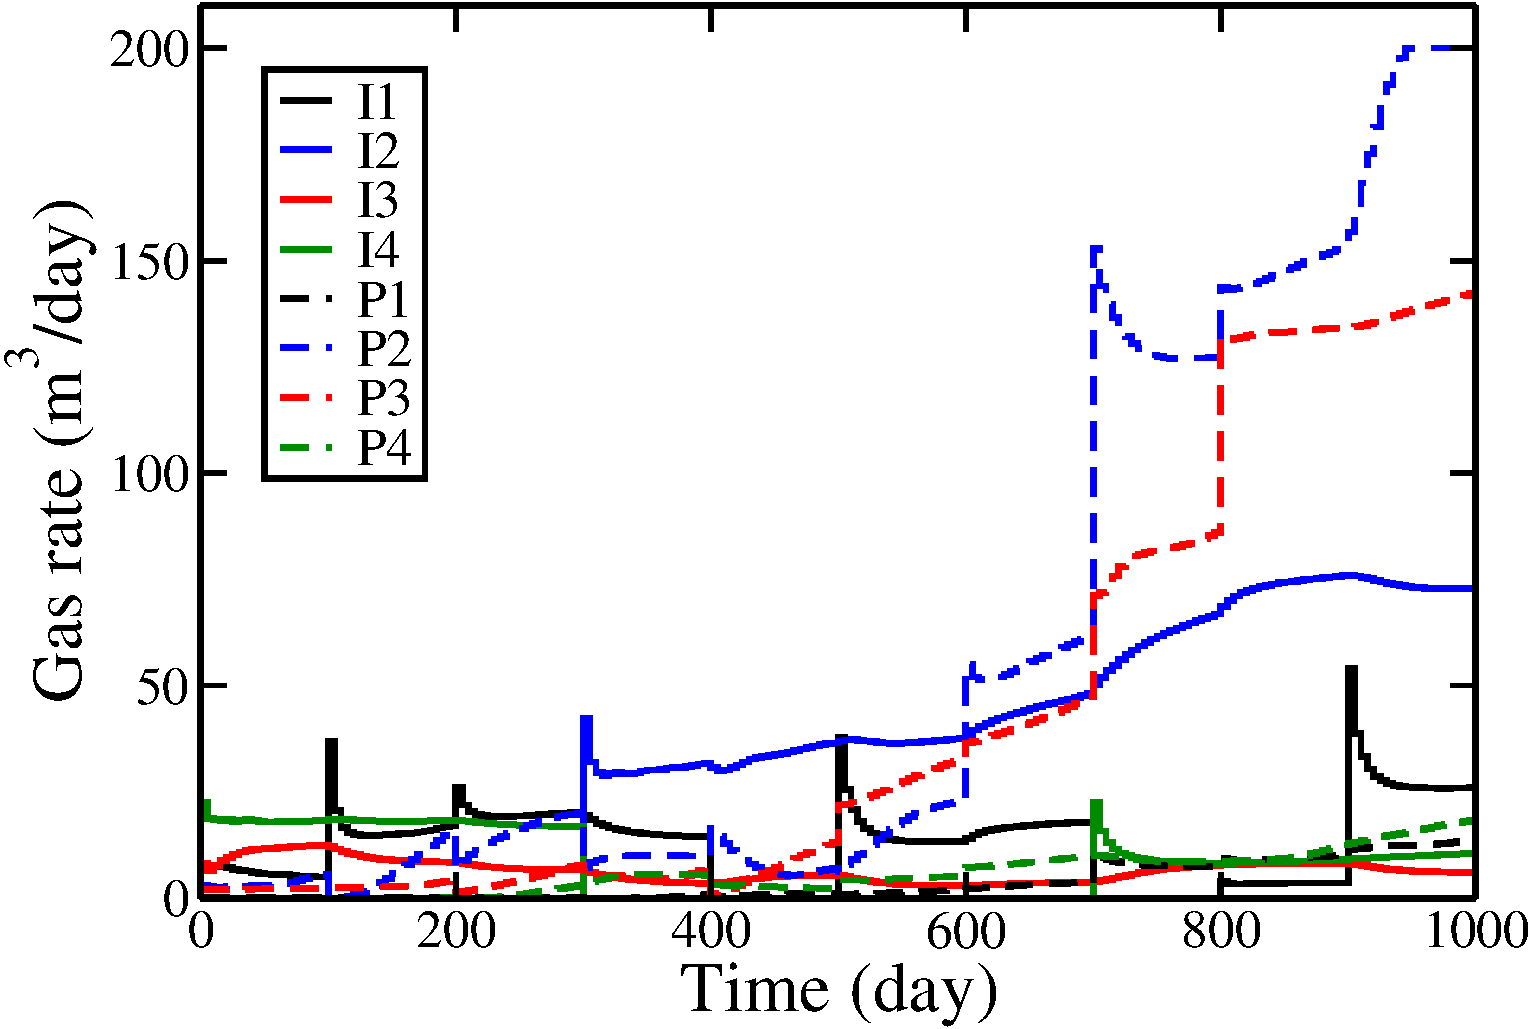
\includegraphics[totalheight=2.17in,angle=0]{spe10topLayerOptimalChoppedIuPu_rate_gas.pdf}
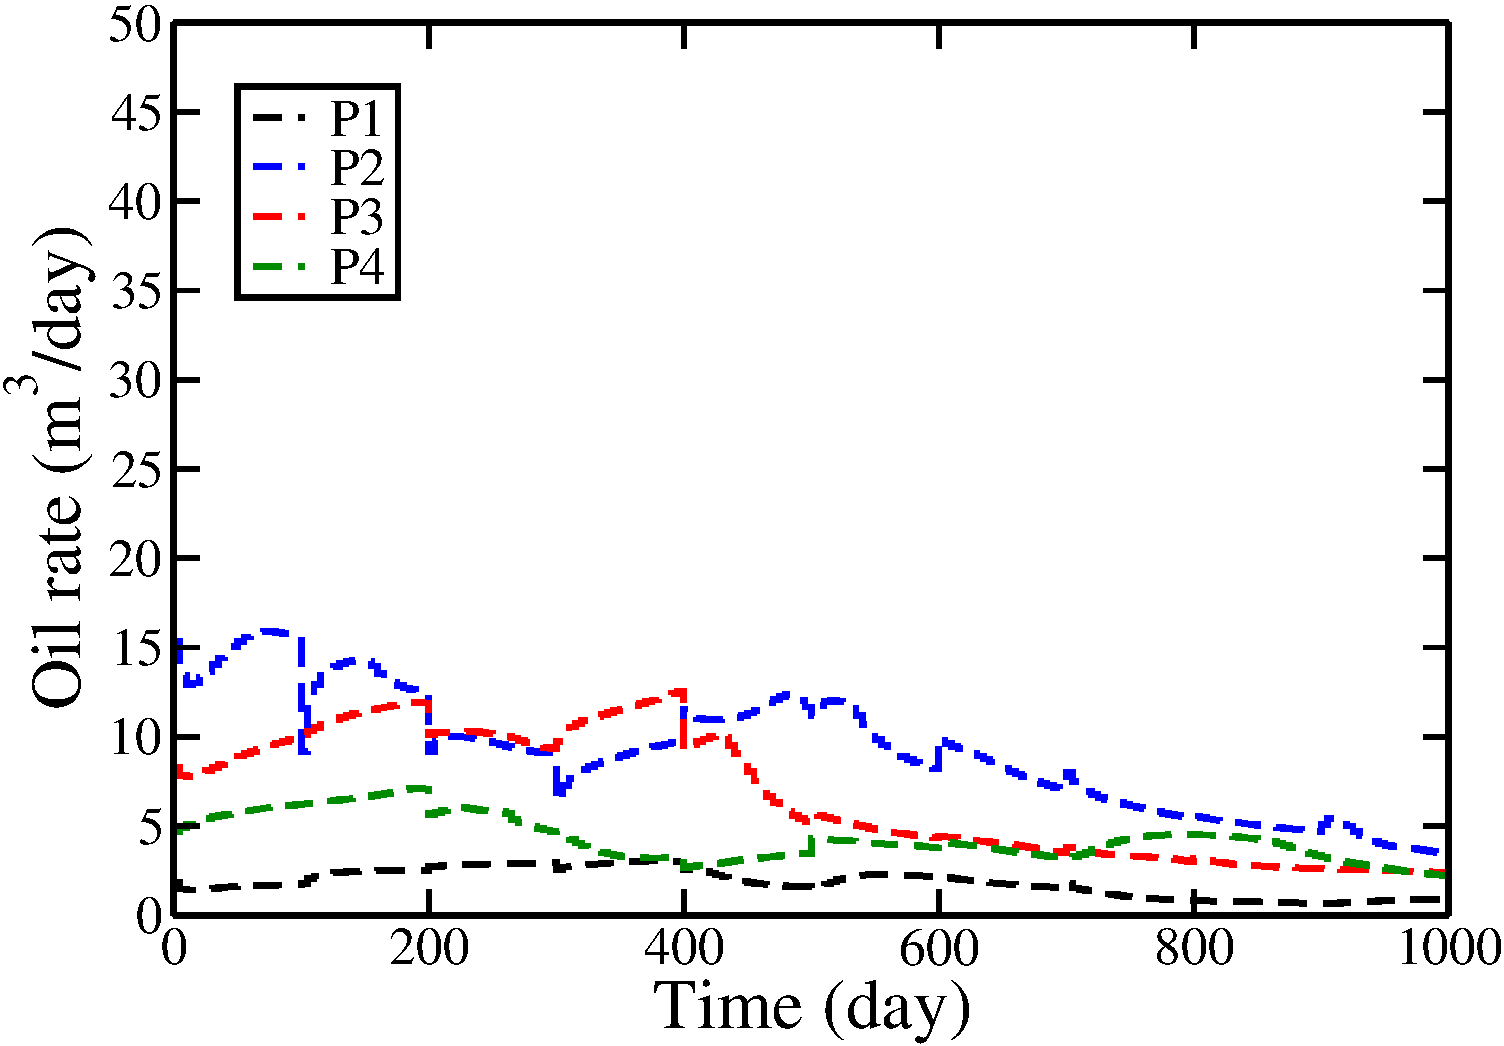
\includegraphics[totalheight=2.2in,angle=0]{spe10topLayerOptimalChoppedIuPu_rate_oil.pdf}
\end{center}
\caption{BHPs (top), gas rates (middle) and oil rates
  (bottom) for the best heuristically constrained solution (Example 2, Run 9).}
\label{fig:SPE10TopLayerUnconstrainedOptimalChoppedRates}
\end{figure}
\begin{figure}
\begin{center}
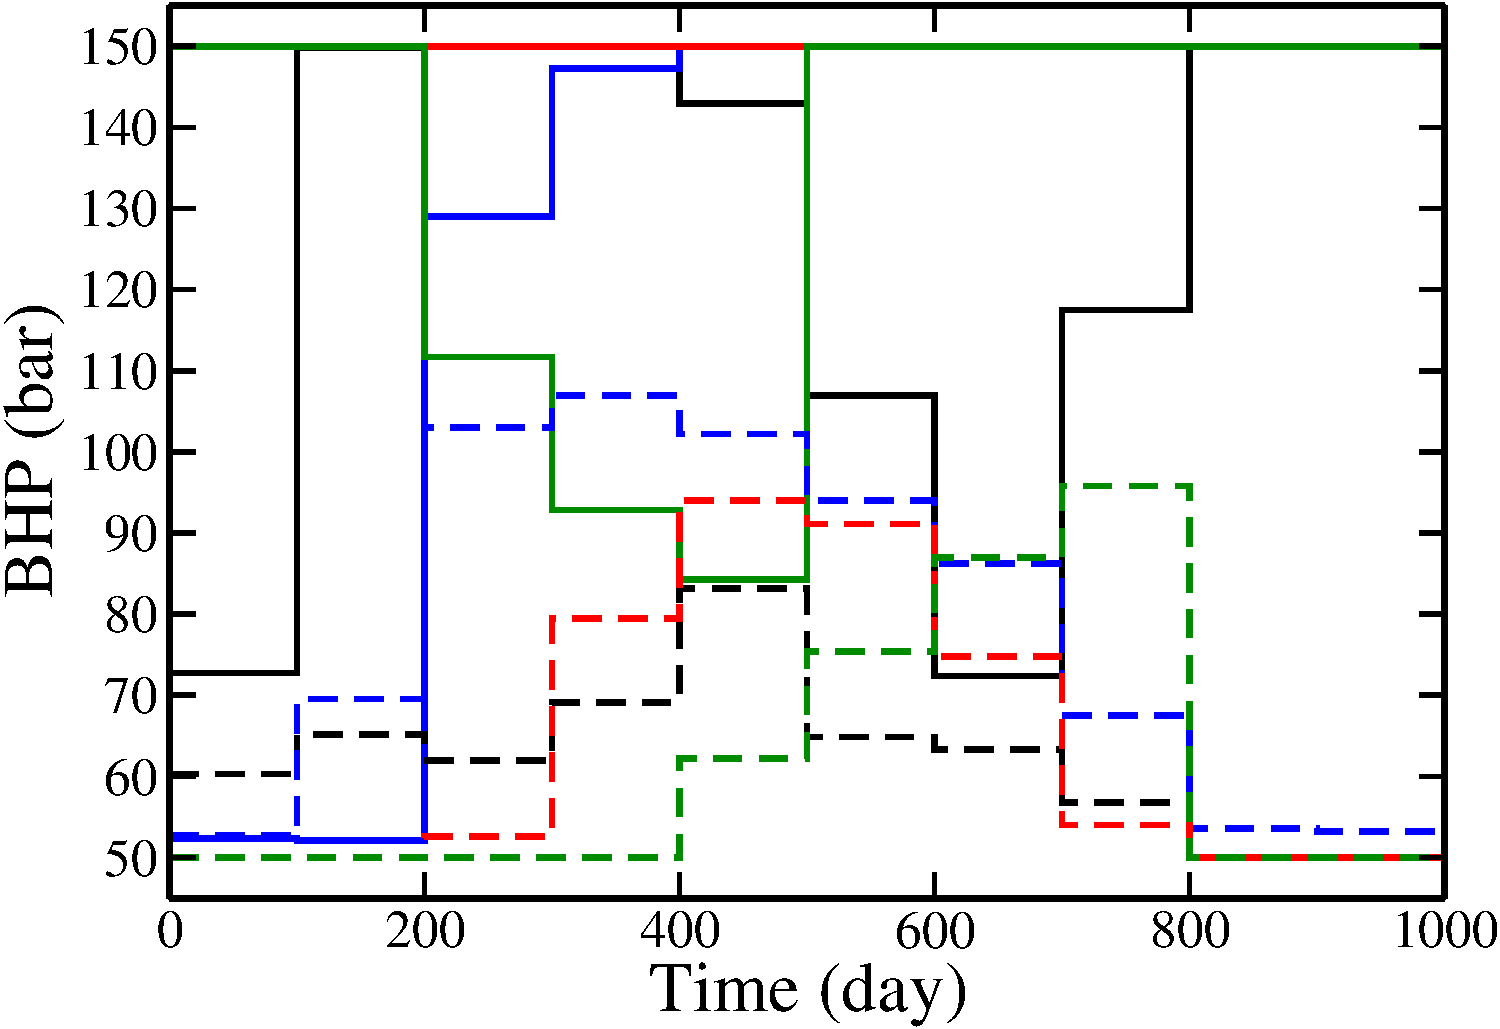
\includegraphics[totalheight=2.2in,angle=0]{spe10TopLayerConstrainedOptimalIuPa_BHP.pdf}
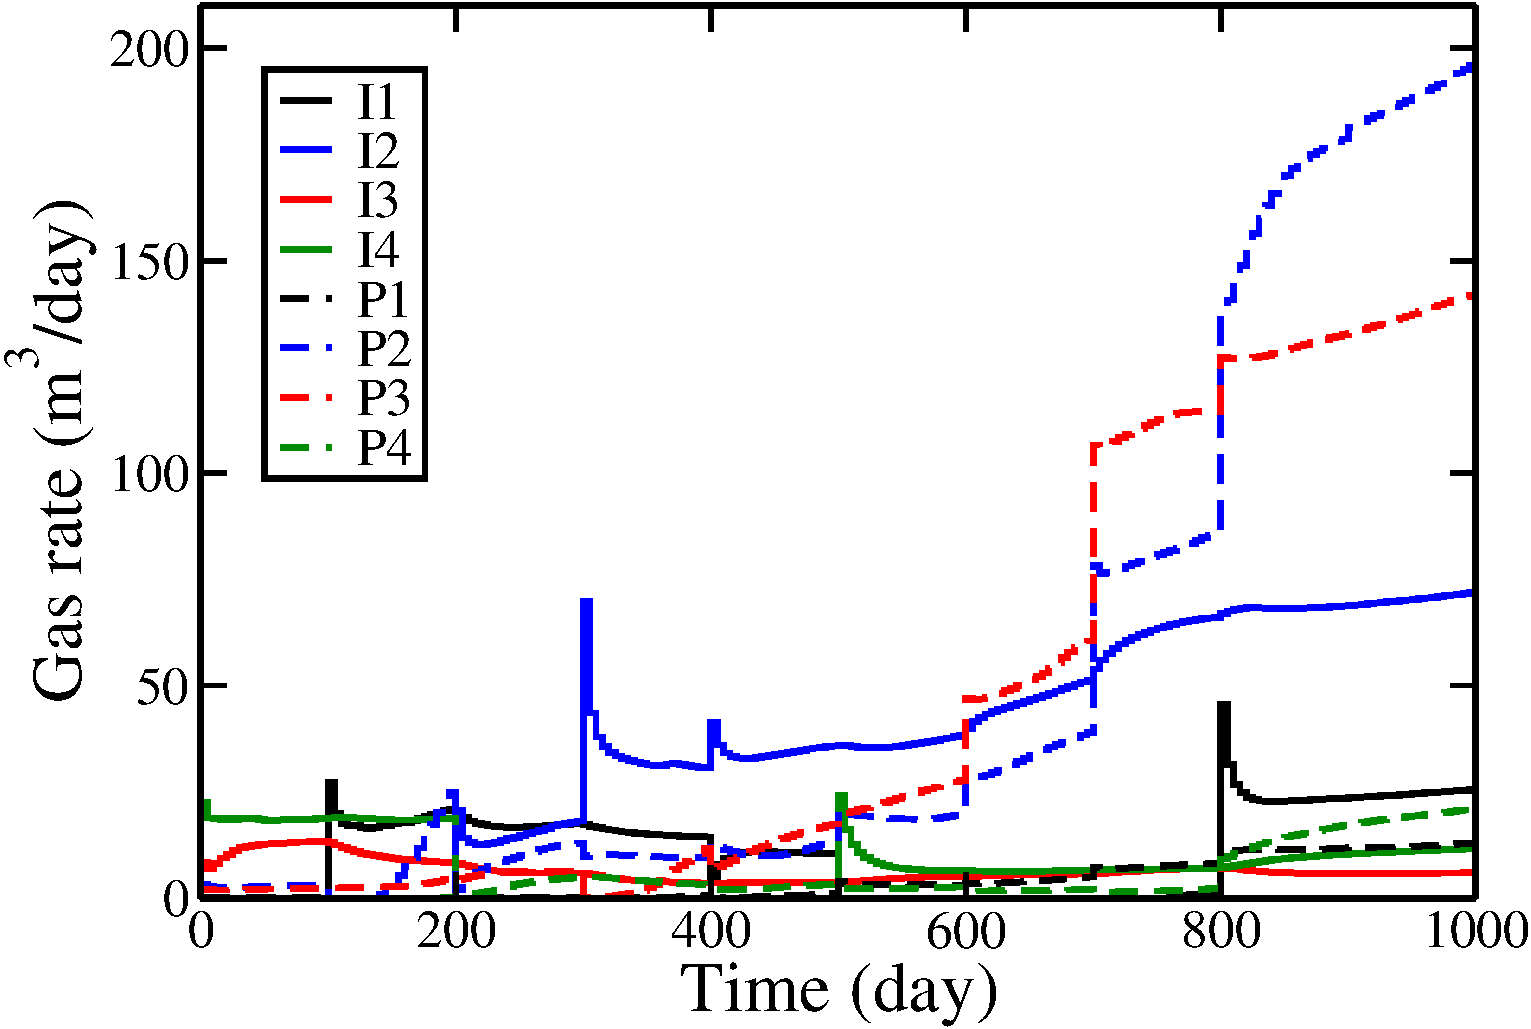
\includegraphics[totalheight=2.2in,angle=0]{spe10TopLayerConstrainedOptimalIuPa_rate_gas.pdf}
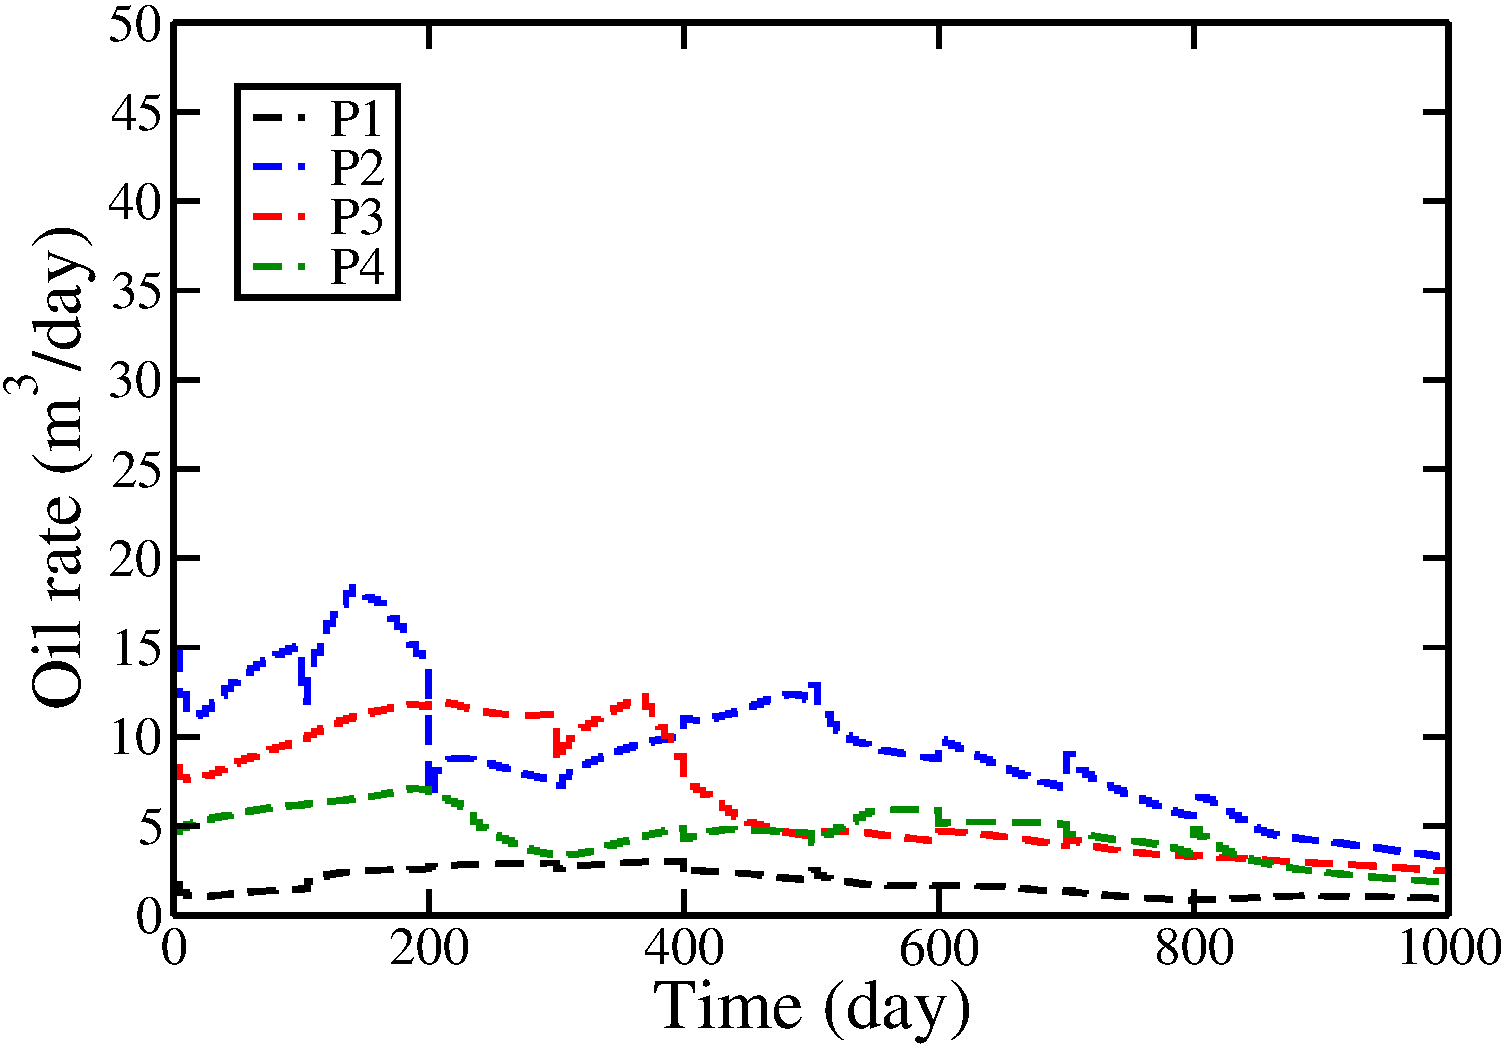
\includegraphics[totalheight=2.2in,angle=0]{spe10TopLayerConstrainedOptimalIuPa_rate_oil.pdf}
\end{center}
\caption{BHPs (top), gas rates (middle) and oil rates
  (bottom) for the best formally constrained solution (Example 2, Run 6).}
\label{fig:SPE10TopLayerConstrainedOptimalRates}
\end{figure}



\subsection{Example 3: Twelve-well channelized system}


Our third example uses the three-dimensional geological model introduced by
\cite{VanEssen}. We again consider CO$_2$ injection, though this model
contains a total of six components, defined in
Table~\ref{table:VanEssenModelFluid}. Further details are given in Table~\ref{table:VanEssenModelReservoir}.  A map of
the $x$-component of permeability (here $\tens{K}_x = \tens{K}_y = 10\tens{K}_z$), along with the
locations of the wells, is shown in Fig.~\ref{fig:VanEssenModelPermeabilityAndWells}.


\begin{figure}[ht]
     \begin{center}
      \begin{tabular}{cccccccc}
      53.90 & 108.0 & 216.5 & 433.9 & 569.6 & 1743 & 3493 & 7000 
      \end{tabular}
       
\includegraphics[width=8cm,height=0.5cm]{VanEssenModelPermeabilityMapColorBar.png}
                                                            
       \medskip
       
       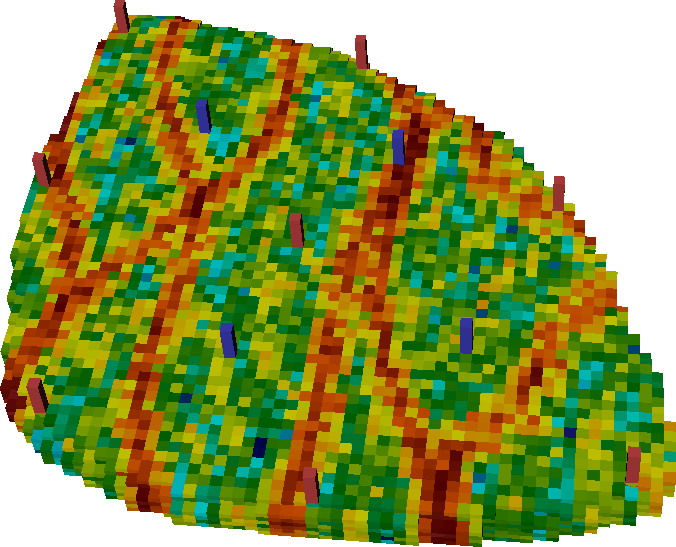
\includegraphics[width=8cm]{VanEssenModelPermeabilityMapConstant.png}%VanEssenModelPermeabilityMap.png}
%       \includegraphics[totalheight=10.5cm]{pdf/VanEssenModelPermeabilityXLogTransparent.pdf}
     \end{center}
     \caption{Reservoir model and wells for Example 3 (from \cite{VanEssen}). Background shows $\log \tens{K}_x$.}
  \label{fig:VanEssenModelPermeabilityAndWells}
\end{figure}


\begin{table}
\centering
\caption{Fluid description for Example 3}
\begin{tabular}{|l|r|r|r|r|r|r|}
%\hline
%\multicolumn{7}{|c|}{SPE10 top layer}    \\
\hline
Component            & CO$_2$ & C$_1$ & C$_2$ & C$_3$ & C$_4$  & C$_{10}$ \\
\hline
Initial comp. (\%)   & 1    & 20  & 30  & 19  & 10   & 20     \\
Injection comp. (\%) & 95   &  1  &  1  &  1  &  1   &  1     \\
\hline
\end{tabular}
\label{table:VanEssenModelFluid}
\end{table}

\begin{table}
\centering
\caption{Model parameters for Example 3}
\begin{tabular}{|l|rr|}
\hline
Grid size                       & 60 $\times$ 60 $\times$ 7        &           \\
\hline\hline
Parameter                      & Value           & Units     \\
\hline
\hline
$\Delta x$                     & 24           & m            \\
$\Delta y$                     & 24           & m            \\
$\Delta z$                     &  4           & m            \\
Depth                          & 2538       & m            \\
Initial pressure               & 100          & bar          \\
Temperature                    & $372$     & $^\circ$C    \\
Rock compressibility           & $10^{-5}$    & 1 / bar      \\
Simulation time                & 300          & d            \\
Pressure upper bound           & 120          & bar          \\
Pressure lower bound           &  90          & bar          \\
\hline
Residual gas saturation  & 0 & -                             \\
Residual oil saturation  & 0 & -                             \\
End point rel perm gas   & 1 & -                             \\
End point rel perm oil   & 1 & -                             \\
Corey exponent gas       & 2 & -                             \\
Corey exponent oil       & 2 & -                             \\
      \hline\hline
Well locations [grid block no.] & $i$ & $j$                      \\
\hline
Injector 1               &  5 &  57                          \\
Injector 2               &  30&  53                          \\
Injector 3               &   2&  35                          \\
Injector 4               &  27&  29                          \\
Injector 5               &  50&  35                          \\
Injector 6               &   8&   9                          \\
Injector 7               &  32&   2                          \\
Injector 8               &  57&   6                          \\
Producer 1               &  16&  43                          \\
Producer 2               &  35&  40                          \\
Producer 3               &  23&  16                          \\
Producer 4               &  43&  18                          \\
\hline
\end{tabular}
\label{table:VanEssenModelReservoir}
\end{table}


The control parameters of our optimization problem are again the well BHPs.  The
wells are constrained to operate between an upper bound of 120~bar and a lower
bound of 90~bar. We also specify nonlinear constraints on both injection and
production in the form of maximum gas flow
rates of 200,000~m$^3/$d for the injectors and 40,000~m$^3/$d for the producers
(both at reservoir conditions). This model is run for a total of 100 days, and
we control the BHPs at initial time and then every ten days (the simulation time
frame is short in this case because the problem specification is such that oil
is produced quickly). There are a total of 120 control parameters in this
problem, and our objective is again to maximize cumulative oil production.

We simulate this model using the same procedures as in the previous examples.
Results for the nine runs for each case are presented in
Table~\ref{table:vanessen}. The feasible reference case yields 5.030$\times 10^6$~m$^3$ of
oil, while the best heuristically constrained case (Run 2) provides 5.457$\times 10^6$~m$^3$
of oil, an improvement of 8.5\%. The best formally constrained case (Run 3)
achieves an optimum of 5.306$\times 10^6$~m$^3$ of oil, which exceeds the reference case by
5.5\% but is less than the best heuristic case. The oil production profiles
for the best runs, along with the feasible reference case, are shown in
Fig.~\ref{fig:VanEssenRevenue}. We again see that the early time production in
the reference case exceeds that of the optimized cases, though the cumulative
oil produced in the optimized cases is of course higher. 

In this example, the formal constraint handling approach typically required about 1.5 times the
number of forward simulations as were required using the heuristic treatment.
Our findings for this example clearly illustrate the potential
advantages of the heuristic treatment for complex optimization problems involving multiple wells
operating under nonlinear constraints.




\begin{table}
\centering
\caption{Oil production in $10^6$~m$^3$ (Example 3) for the optimized objective function
         without satisfying the nonlinear constraints (`Unconstr.'), satisfying the nonlinear constraints
         using the heuristic treatment (`Heuristic'), and satisfying the nonlinear constraints
         using the formal approach (`Formal'). Best feasible results shown in bold.}
\begin{tabular}{|c|c|c|c|}
\hline
 Run              & Unconstr. & Heuristic & Formal     \\
\hline
Reference         & 5.030 &  5.030    &          \\
1 & 5.450 &  5.449   &  5.284   \\
2 & 5.467 &\bf{5.457} &  5.294   \\
3 & 5.171 &  5.171   &\bf{5.306}\\
4 & 5.288 &  5.287   &  5.132   \\
5 & 5.424 &  5.423   &  5.224   \\
6 & 5.344 &  5.348   &  5.260   \\
7 & 5.321 &  5.230   &  4.994   \\
8 & 5.207 &  5.205   &  5.196   \\
9 & 5.353 &  5.349   &  4.986   \\
\hline
\end{tabular}
  \label{table:vanessen}
\end{table}


%1 & O30G23 5.450    &  5.2976    &  O41G30 5.284         \\
%2 & O47G27 5.467    &\bf{5.46} &  O46G30 5.294         \\
%3 & O22G12 5.171    &  5.02    &  O44G30 \bf{5.306}    \\
%4 & O25G18 5.288    &  5.02    &  O28G13 5.132         \\
%5 & O43G27 5.424    &  5.29    &  O35G30 5.224         \\
%6 & O43G19 5.344    &  5.35    &  O48G38 5.260         \\
%7 & O31G18 5.321    &  5.20    &  O43G29 4.994         \\
%8 & O19G10 5.207    &  5.21    &  O37G25 5.196         \\
%9 & O13G10 5.353    &  5.19    &  O91G26 4.986         \\


\begin{figure} [ht]
\begin{center}
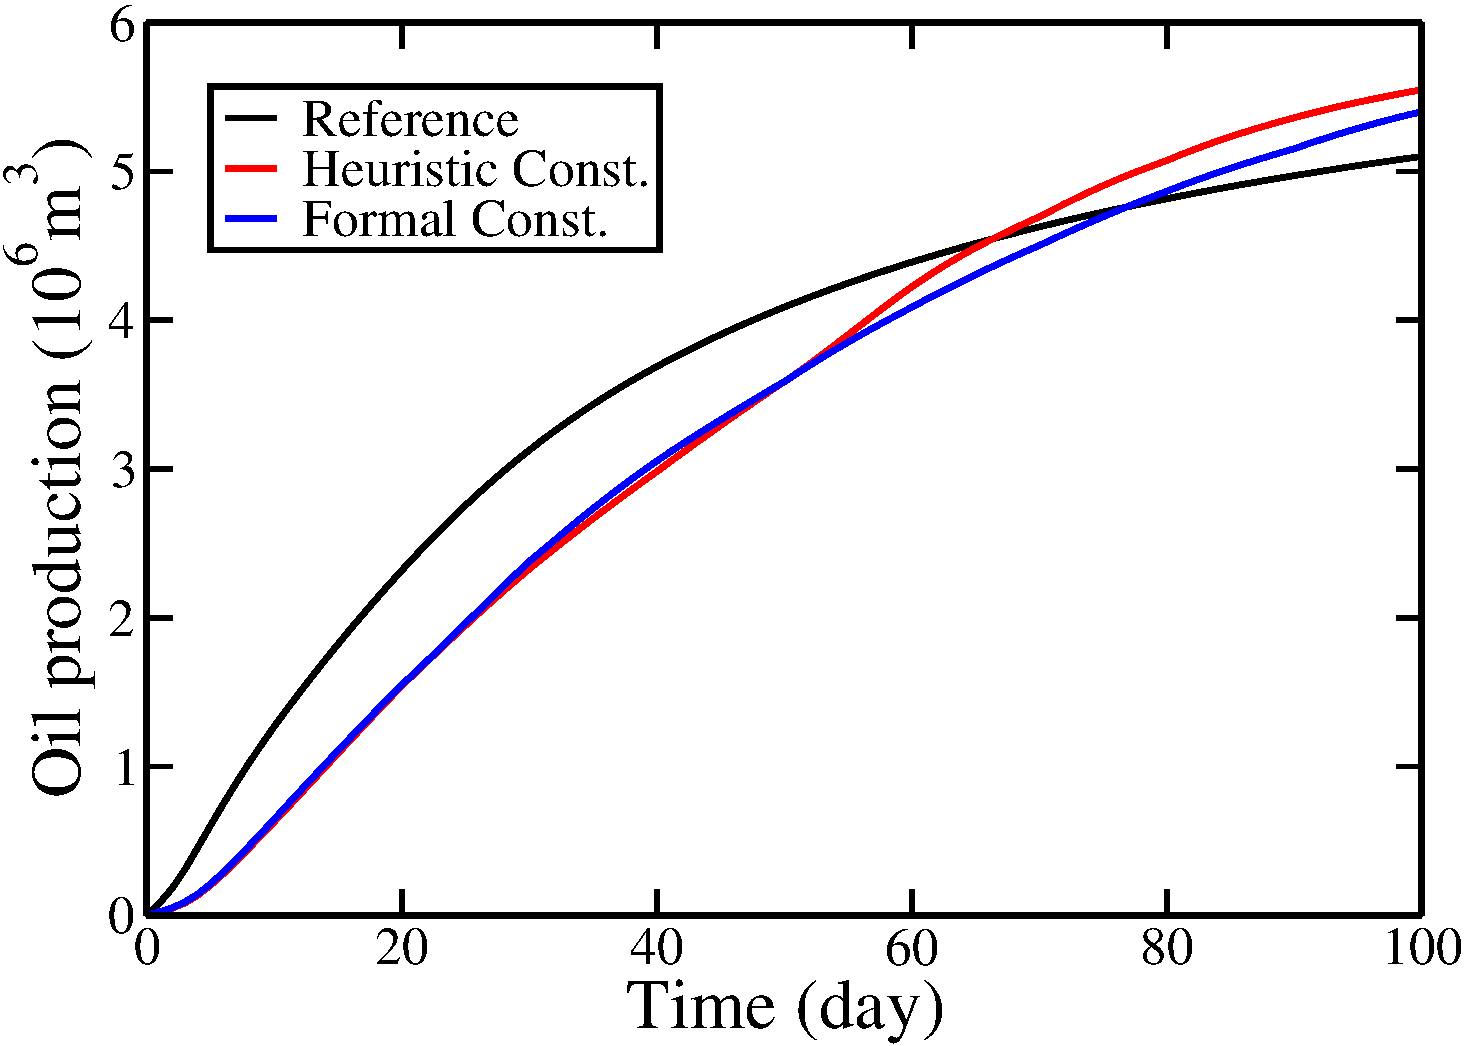
\includegraphics[totalheight=2.2in,angle=0]{vanEssenRevenue.pdf}
\end{center}
\caption{Oil production versus time for Example 3. Results are for
  feasible reference case (black curve), best heuristically constrained solution (Run 2, red curve)
  and best formally constrained solution (Run 3, blue curve).}
\label{fig:VanEssenRevenue}
\end{figure}



\subsection{Example 4: Norne model}

In our final example we consider the Norne benchmark problem, which is a model
of a real field located offshore Norway~\cite{NorneWebsite}. The actual Norne
model involves a three-phase black-oil system. Here we use the prescribed Norne
geological model and well positions (for wells that were operational in January 2005 in the original model). The Norne model
contains 29 wells, as shown in Fig.~\ref{fig:NorneModelAndWells}, though our
model involves only 28 of these wells (we do not include the injector C-4H
because it does not operate from 2005-2008). Instead of
black-oil, we consider a five-component compositional system with CO$_2$
injection (see Table~\ref{table:NorneModelFluid} for the fluid description). The
model contains a total of 113,344 grid blocks, though only 44,431 of these
blocks are active.  Other model parameters are provided in
Table~\ref{table:NorneReservoir}.


\begin{figure}[ht]
     \begin{center}
%      \includegraphics[totalheight=5cm]{Norne/Norne1.png}
     \begin{tabular}{cccccccc}
      0.66 & 2.275 & 7.963 & 27.45 & 95.36 & 331.2 & 1151 & 3997
      \end{tabular}
       
\includegraphics[width=8cm, height=0.5cm]{VanEssenModelPermeabilityMapColorBar.png}
       
       \medskip
      
       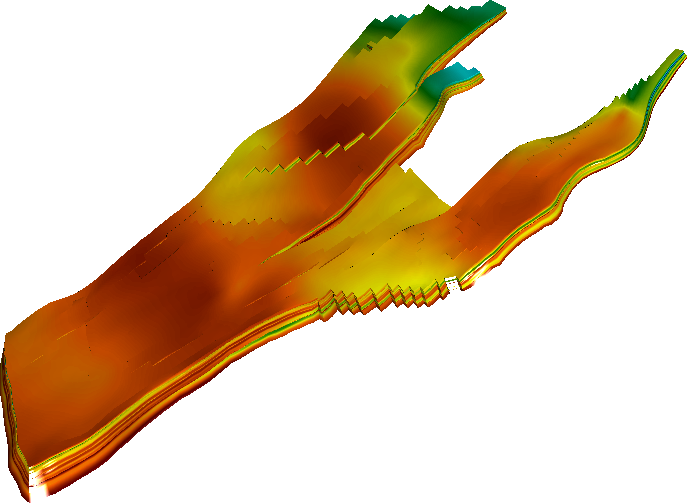
\includegraphics[totalheight=5cm]{NorneModelPermeabilityMap.png}
%       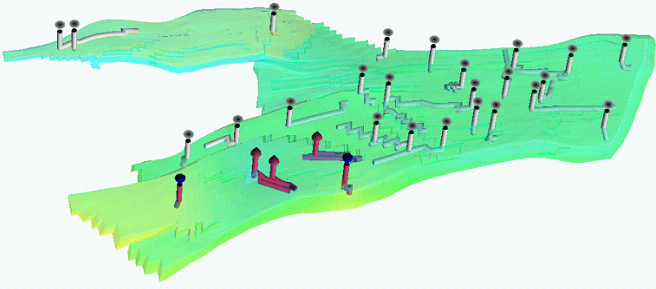
\includegraphics[totalheight=3.5cm]{Norne3.png}
     \end{center}
     \caption{Permeability field in log scale for Example 4 (Norne model).}
  \label{fig:NorneModelAndWells}
\end{figure}


\begin{table}
\centering
\caption{Fluid description for Example 4}
\begin{tabular}{|l|r|r|r|r|r|}
\hline
Component            & CO$_2$ & NC$_4$ & C$_8$ & C$_1$ & C$_{15}$  \\
\hline
Initial composition (\%)   & 1    & 9  & 40  & 10  & 40   \\
Injection composition (\%) & 90   & 7  &  1  &  1  &  1  \\
\hline
\end{tabular}
\label{table:NorneModelFluid}
\end{table}

\begin{table}
\centering
\caption{Model parameters for Example 4 (Norne model)}
\begin{tabular}{|l|rr|}
\hline
Grid size                & 46 $\times$ 112 $\times$ 22 &           \\
\hline\hline
Parameter                & Value    & Units \\
\hline
\hline
$\Delta x$               & 24        & m    \\
$\Delta y$               & 24        & m    \\
$\Delta z$               &  4        & m    \\
Depth                    & 3000      & m    \\
Initial pressure         & 100       & bar  \\
Temperature              &$372$      & $^\circ$C \\
Rock compressibility     &$8 \times 10^{-5}$ & 1 / bar \\
Simulation time          &300        & d          \\
Pressure upper bound     & 150       & bar      \\
Pressure lower bound     &  50       & bar      \\
\hline
Residual gas saturation  & 0    & -    \\
Residual oil saturation  & 0    & -    \\
End point rel perm gas   & 1    & -    \\
End point rel perm oil   & 1    & -    \\
Corey exponent gas       & 2    & -    \\
Corey exponent oil       & 2    & -    \\
\hline
\end{tabular}
\label{table:NorneReservoir}
\end{table}


\begin{table}
\centering
\caption{Oil production in $10^6$~m$^3$ (Example 4) for the optimized objective function
         without satisfying the nonlinear constraints (`Unconstr.'), satisfying the nonlinear constraints
         using the heuristic treatment (`Heuristic'), and satisfying the nonlinear constraints
         using the formal approach (`Formal'). Best feasible results shown in bold.}
\begin{tabular}{|c|c|c|c|}
\hline
Run               & Unconstr. & Heuristic & Formal  \\
\hline
Reference         & 252.0         & 142.0          &             \\
1  & 270.2            & 146.0          & \bf{138.5}        \\
2  & 266.7            & 143.3          & 138.3    \\
3  & 261.6            & 124.3          & 129.3          \\
4  & 270.3            & \bf{147.8}   & 137.5         \\
5  & 270.7            & 146.5          & 138.0    \\
6  & 268.8            & 146.8          & 137.8 \\
7  & 270.4            & 146.2          & 129.7         \\
8  & 270.8            & 146.8          & 129.9      \\
9  & 270.6            & 146.2          & 136.6       \\
\hline
\end{tabular}
  \label{table:Norne}
\end{table}

% max{delta} = 2 days
%1  & O42G23 270.2 & 146          & 125         \\
%2  & O57G23 265.7 & 143          & \bf{130}    \\
%3  & O54G28 261.6 & 120          & 88          \\
%4  & O46G28 270.3 & \bf{147.77}     & 121         \\
%5  & O15G12 270.7 & 147          & \bf{130}    \\
%6  & O50G27 268.8 & 145          & 119         \\
%7  & O22G12 270.4 & 146          & 129         \\
%8  & O26G16 270.8 & 147          & 119         \\
%9  & O54G18 270.6 & 147          & 109         \\
% 366 total iters, 40.6 average unconstrained


\begin{figure} [ht]
\begin{center}
\includegraphics[totalheight=2.18in,angle=0]{NorneRevenue.pdf}
\end{center}
\caption{Oil production versus time for Example 4. Results are for
  feasible reference case (black curve), best heuristically constrained solution (Run 4, red curve)
  and best formally constrained solution (Run 2, blue curve).}
\label{fig:NorneRevenue}
\end{figure}



The control parameters for the optimization are again the well BHPs, constrained
to lie between 50~bar and 150~bar. The nonlinear constraints are maximum gas
injection rate of $10^5$~m$^3/$d at reservoir conditions for each injector. The
simulation is run for 300 days, and we control the BHPs at initial time and then
every 30 days thereafter. Because this problem involves 28 wells, there are 280
control parameters. Our objective is to maximize cumulative oil production.

Results for the three sets of runs are reported in Table~\ref{table:Norne}. It
is evident from the large differences between the nonlinearly unconstrained runs
(second column) and the constrained runs (third and fourth columns) that the
nonlinear constraints have a large effect in this example. Applying these constraints heuristically, the best maximum obtained is
147.8$\times 10^6$~m$^3$ (Run~4), an improvement of 4.2\% over the heuristically constrained
reference case. This level of improvement is less than that observed for the
other examples. We also see that the formal constraint handling approach leads
to a result for cumulative oil production (138.5$\times 10^6$~m$^3$ in the best case, Run~1)
that is lower than that for the heuristic reference case, which does
not involve any optimization. The results using the formal treatment illustrate the potential challenges that can
arise in complex problems with large numbers of control parameters and many active nonlinear
constraints. It is worth reiterating that the heuristic approach does, even in
this challenging case, provide improvement over the feasible reference solution.

The oil production profiles for the best optimization runs, along with the
feasible reference case, are shown in Fig.~\ref{fig:NorneRevenue}. The slight
improvement offered by the heuristic procedure over the reference case is
evident. The detailed BHP and gas injection rates (for some of the wells) versus time for the three
cases are shown in Figs.~\ref{fig:NorneReferenceRates},
\ref{fig:NorneUnconstrainedOptimalChoppedRates} and
\ref{fig:NorneConstrainedOptimalRates}. The frequent shifts in BHP in the
reference case (Fig.~\ref{fig:NorneReferenceRates}) and in the heuristic
case (Fig.~\ref{fig:NorneUnconstrainedOptimalChoppedRates}) enable higher
oil production in those runs. In the formally constrained case
(Fig.~\ref{fig:NorneConstrainedOptimalRates}), BHPs must be held constant over
the entire control period. This results in less gas injection and, as a
result, less oil production than in the other cases.


We expect that the use of a sufficiently large number of control periods would
provide improvement in the results using the formal constraint handling
procedure. This would lead, however, to a more challenging optimization problem
that might require many more forward simulations. For the results presented
here, the optimizations using formal constraint handling required about 150
forward simulations on average. Optimizations using the heuristic constraint
handling, by contrast, required about 41 forward simulations on average. Thus we
again observe significant improvements in computational efficiency using the
heuristic approach.


\begin{figure}
\begin{center}
\includegraphics[totalheight=2.2in,angle=0]{norneReferenceChoppedT300_BHP.pdf}
\includegraphics[totalheight=2.2in,angle=0]{norneReferenceChoppedT300_rate_gas.pdf}
\end{center}
\caption{Injector BHPs (top) and gas injection rates (bottom) for the feasible reference solution (Example 4).}
\label{fig:NorneReferenceRates}
\end{figure}


\begin{figure}
\begin{center}
\includegraphics[totalheight=2.2in,angle=0]{norneOptimalChoppedImPbT300_BHP.pdf}
\includegraphics[totalheight=2.2in,angle=0]{norneOptimalChoppedImPbT300_rate_gas.pdf}
\end{center}
\caption{Injector BHPs (top) and gas injection rates (bottom) for the best heuristically constrained solution (Example 4, Run 4).}
\label{fig:NorneUnconstrainedOptimalChoppedRates}
\end{figure}


\begin{figure}
\begin{center}
\includegraphics[totalheight=2.2in,angle=0]{norneConstrainedIlPlT300_BHP.pdf}
\includegraphics[totalheight=2.2in,angle=0]{norneConstrainedIlPlT300_rate_gas.pdf}
\end{center}
\caption{Injector BHPs (top) and gas injection rates (bottom) for the best formally constrained solution (Example 4, Run 1).}
\label{fig:NorneConstrainedOptimalRates}
\end{figure}



\section{Concluding remarks}  \label{sec:conclusions}
In this work we formulated and tested an adjoint-based optimization procedure
for compositional reservoir simulation. The method we employed was implemented into
Stanford's Automatic Differentiation-based General Purpose Research Simulator
(AD-GPRS). The use of automatic differentiation simplifies the adjoint
implementation and subsequent code enhancements. Two different treatments for
handling nonlinear constraints were presented. In the formal constraint handling
procedure, lumped constraints and their gradients are provided to the optimizer,
and feasibility is enforced by the optimization algorithm. In the second
(heuristic) procedure, an optimization satisfying only the bound and linear
constraints is performed first. Then, the forward model is run using the
controls from the first stage, but the simulator is allowed to switch from BHP
to rate control (for a problem in which BHPs are the control variables) as
required to satisfy the nonlinear rate constraints.


Numerical results were presented for four example cases of increasing
complexity. Nine runs, starting from different initial conditions, were
performed in all cases, for both the heuristic and the formal nonlinear
constraint treatments. In our examples, the control variables were the time-varying well BHPs, and maximum injection or production rate specifications entered as nonlinear
constraints. The total number of control variables ranged from 40 to 320. Improvement in cumulative oil produced (which was the objective function in all cases) using our optimization procedures ranged from 4.2\% to 11.6\% relative to the reference solutions. 

In the simplest case (Example~1), the formal constraint handling approach was shown to outperform the heuristic procedure when we increased the number of control variables from 40 to 320. In the next (somewhat more complicated) case, Example~2, the formal constraint treatment continued to outperform the heuristic procedure, though its advantage was very slight. In the other two cases, which were more challenging in terms of model size and number of wells (and they involved three-dimensional models, while the first two examples were two-dimensional), the heuristic treatment provided better objective function values than the formal approach. 

These observations suggest that, although the formal constraint handling approach is theoretically superior, complications related to constraint lumping and the existence of poor local optima (and the additional complexity inherent in problems with large numbers of optimization variables and nonlinear constraints) may render the formal procedure less effective than the heuristic approach in challenging cases. Thus, though we expect (and observe) the formal procedure to be the method of choice in relatively simple cases, the heuristic approach should be considered for use in more complex problems. It may even be beneficial to apply some type of hybrid technique, where the result from the heuristic approach is used as the initial guess for the formal procedure. It is also important to note that the heuristic constraint treatment was found to be much more efficient than the formal approach. 


In addition to the discrete adjoint procedure, which was used for all of the
examples presented in this paper, we also derived and implemented a continuous
adjoint formulation. We showed that the two formulations use different
final time conditions and as a result the gradients do not
agree in general. However, the two boundary conditions become almost identical as the
size of the last time step approaches zero, in which case the gradients obtained by
both formulations are essentially the same.

There are a number of areas in which future research should be directed. Other
treatments for nonlinear constraints, both formal and heuristic, should be
considered, and the relative benefits of controlling rates instead of BHPs
should be assessed. It will be of interest to apply the general optimization
framework to larger and more realistic simulation models. Other types of wells
(horizontal, deviated, multilateral) should also be considered, along with the
optimization of downhole inflow control devices. The overall approach can be 
extended to perform robust control (to account for geological uncertainty) and hierarchical
(multi-objective) control to balance long-term and short-term objectives. Finally, our procedures could be applied for the optimization of CO$_2$ storage or for combined
EOR-CO$_2$ storage operations.



\begin{acknowledgements} 
We thank Denis Voskov and Oleg Volkov at Stanford
University for useful discussions and assistance with AD-GPRS.
We also thank Michael Saunders for his support 
on SNOPT. We are grateful
to the sponsors of the Stanford University Smart Fields Consortium for partial
funding of this work.
\end{acknowledgements}



% BibTeX users please use one of
%\bibliographystyle{spbasic}      % basic style, author-year citations
\bibliographystyle{spmpsci}      % mathematics and physical sciences
%\bibliographystyle{spphys}       % APS-like style for physics
\bibliography{ComputationalGeosciencesAdjoints}



\end{document}
